\pdfoutput=1 % required by arXiv
% twocolumn - singlespace
\documentclass[journal]{IEEEtran}
\newif\iffinal
\finaltrue

%% onecolumn - doublesplaced - for review
%\documentclass[11pt,onecolumn,draftcls,journal]{IEEEtran}
%\usepackage[figuresonly]{endfloat} %% required endfloat package version 2.5 for figuresonly option to work
%\newif\iffinal
%\finalfalse



%\usepackage{ifpdf}
% \ifpdf
%   % pdf code
% \else
%   % dvi code
% \fi
%\usepackage{cite}

\ifCLASSINFOpdf
  \usepackage[pdftex]{graphicx}
  % declare the path(s) where your graphic files are
  \graphicspath{{./figs/}{./jpeg/}}
  \DeclareGraphicsExtensions{.pdf,.png}
\else
  % \usepackage[dvips]{graphicx}
  % \graphicspath{{../eps/}}
  % \DeclareGraphicsExtensions{.eps}
\fi
\usepackage[utf8]{inputenc}
\usepackage{flushend}
\usepackage{enumerate}

%\usepackage[cmex10]{amsmath}
%\usepackage{algorithmic}
%\usepackage{array}
\ifCLASSOPTIONcompsoc
  \usepackage[caption=false,font=normalsize,labelfont=sf,textfont=sf]{subfig}
\else
  \usepackage[caption=false,font=footnotesize]{subfig}
\fi
%\usepackage{fixltx2e}
%\usepackage{stfloats}
%\fnbelowfloat
%\usepackage{dblfloatfix}
%\ifCLASSOPTIONcaptionsoff
%  \usepackage[nomarkers]{endfloat}
% \let\MYoriglatexcaption\caption
% \renewcommand{\caption}[2][\relax]{\MYoriglatexcaption[#2]{#2}}
%\fi
\usepackage{url}
\usepackage{hyperref}
\usepackage{balance}

\usepackage{multirow} % - Giovani - 27/06/2014
\usepackage{marvosym} % - Giovani - 03/07/2014

%%% for ToDo command - colored edition
\usepackage{color,colortbl}
\usepackage{hhline}
\definecolor{DarkGray}{rgb}{0.25,0.25,0.25}
\definecolor{LightGray}{rgb}{0.75,0.75,0.75}

\usepackage[table]{xcolor}
\newcommand{\TODO}[1]{\textcolor{black}{[\textbf{TODO: #1}]}}
\newcommand{\ToDo}[1]{\textcolor{black}{[\textbf{ToDo: #1}]}}
\newcommand\blue[1]{{\color{black}#1}}
\newcommand\red[1]{{\color{black}{#1}}}

\newcommand\rva[1]{{\color{black}{#1}}}
\newcommand\rvg[1]{{\color{black}{#1}}}
\newcommand\rrv[1]{{\color{black}#1}}
\newcommand\question[2]{{\color{red}{#1}}{\color{black}{ [#2]}}}

\newcommand{\dm}[1]{\textcolor{green}{{\bf{\textsf{\underline{Menotti}: #1\\}}}}}
\newcommand{\DM}[1]{\textcolor{green}{#1\\}}
%%%

\hyphenation{menottid spoofnet}


\begin{document}
\sloppy

% A Unified Framework to Learn Deep Representations for Biometric Spoofing Modalities
% \title{A Unified Framework to Learn Deep Representations for Iris, Face, and Fingerprint Spoofing Attacks}
\title{Deep Representations for Iris, Face, and Fingerprint Spoofing Detection}
% through Convolutional Neural Networks 

\author{David~Menotti\textsuperscript,~\IEEEmembership{Member,~IEEE,}
        Giovani~Chiachia\textsuperscript,
        Allan~Pinto,~\IEEEmembership{Student Member,~IEEE,}
        William~Robson~Schwartz,~\IEEEmembership{Member,~IEEE,}
        Helio~Pedrini,~\IEEEmembership{Member,~IEEE,}\\
        Alexandre~Xavier~Falc\~{a}o,~\IEEEmembership{Member,~IEEE,}
        and~Anderson~Rocha,~\IEEEmembership{Member,~IEEE}% <-this % stops a space
\thanks{D. Menotti, G. Chiachia, A. Pinto, H. Pedrini, A. X. Falc\~{a}o and A. Rocha are with the Institute of Computing (IC), University of Campinas, Campinas (UNICAMP), SP, 13083-852, Brazil. email: menottid@gmail.com, \{chiachia,allan.pinto,helio.pedrini,afalcao,anderson.rocha\}@ic.unicamp.br.}% <-this % stops a space
\thanks{W. R. Schwartz is with the Computer Science Department (DCC), Federal University of Minas Gerais (UFMG), Belo Horizonte, MG, 31270-010, Brazil. email: william@dcc.ufmg.br.}% <-this % stops a space
\thanks{D. Menotti is also with Computing Department (DECOM), Federal University of Ouro Preto (UFOP), Ouro Preto, MG, 35400-000, Brazil (he has spent his sabbatical year (2013-2014) at IC-UNICAMP). email: menotti@iceb.ufop.br.}% <-this % stops a space
\thanks{\textit{(David Menotti and Giovani Chiachia contributed equally to this work.)}}%
}

% The paper headers
\markboth{IEEE Transactions on Information Forensics and Security,~Vol.~XX, No.~XX, April~XXXX}%
{Menotti \MakeLowercase{\textit{et al.}}: Deep Representations for Iris, Face, and Fingerprint Spoofing Detection}
% You can use \ifCLASSOPTIONpeerreview for conditional compilation here if
% you desire.

% If you want to put a publisher's ID mark on the page you can do it like this:
%\IEEEpubid{0000--0000/00\$00.00~\copyright~2012 IEEE}
% Remember, if you use this you must call \IEEEpubidadjcol in the second column for its text to clear the IEEEpubid mark.


% use for special paper notices
%\IEEEspecialpapernotice{(Invited Paper)}

% make the title area
\maketitle


\begin{abstract}
Biometrics systems have significantly improved person
identification and authentication, playing an important role in
personal, national, and global security. However, these systems
might be deceived (or ``spoofed'') and, despite the recent advances
in spoofing detection, current solutions often rely on domain
knowledge, specific biometric reading systems, and attack types. We
assume a very limited knowledge about biometric spoofing at the
sensor to derive outstanding spoofing detection systems for iris,
face, and fingerprint modalities based on two deep learning
approaches.
The first approach consists of learning suitable convolutional 
network architectures for each domain, while the second approach
focuses on learning the weights of the network via back-propagation. We
consider nine biometric spoofing benchmarks --- each one containing
real and fake samples of a given biometric modality and attack type
--- and learn deep representations for each benchmark by combining and
contrasting the two learning approaches. This strategy not only
provides better comprehension of how these approaches interplay, but
also creates systems that exceed the best known results in eight out
of the nine benchmarks. The results strongly indicate that spoofing
detection systems based on convolutional networks can be robust to
attacks already known and possibly adapted, with little effort, to
image-based attacks that are yet to come.

% Biometrics systems have drastically improved person identification
% and/or authentication, playing an important role in personal,
% national, and global security. However, such systems might be
% deceived or ``spoofed'' and, despite the advances in
% spoofing detection to each biometric modality, there is still a lack
% of a clearly unified approach. Aiming at filling this gap, we
% propose a unified framework to learn deep representations for three
% different modalities of spoofing biometrics (i.e., face, iris, and
% fingerprint). The representations are learned directly from the
% data with an optimization procedure that randomly searches for the best
% convolutional neural network from a family of networks defined in a hyperparameter search
% space. Atop these representations, we couple a linear Support Vector Machine
% classifiers for the final
% decision making. Instead of learning thousands and/or millions of
% network weights/parameters based either on back-propagation-like or unsupervised
% feature learning techniques, our networks use random filter weights initialized in a 
% convenient way, which allows us to quickly probe thousands of network configurations.
% Experiments on nine publicly available benchmarks of these 
% three modalities show that our framework achieves either very 
% competitive or state-of-the-art results for all problems and modalities.

% Biometrics systems have drastically improved person identification
% and/or authentication, playing an important role in personal,
% national, and global security. However, such systems might be
% deceived or ``spoofed'' and, despite the advances in
% spoofing detection to each biometric modality, there is still a lack
% of a clearly unified approach. Aiming at filling this gap, we
% propose a unified framework to learn deep representations for three
% different modalities of spoofing biometrics (i.e., face, iris, and
% fingerprint). The representations are learned directly from the
% data, as statistical models of the distributions of the
% real and fake classes, using convolutional neural networks. On the
% top of these representations, we couple a Support Vector Machine
% classifier with linear kernel and hard margins for the final
% decision making. Instead of learning thousands and/or millions of
% network weights/parameters, based either on back-propagation-like or unsupervised
% learning techniques, we focus on the random optimization of the
% network architecture with zero-mean and unit-norm uniform random
% weights. Experiments on nine publicly available benchmarks of these 
% three modalities show that our framework achieves either very 
% competitive or state-of-the-art results for all problems and modalities.
\end{abstract}

% Note that keywords are not normally used for peerreview papers.
\begin{IEEEkeywords}
Deep Learning, Convolutional Networks, Hyperparameter Architecture Optimization, Filter Weights Learning, Back-propagation, Spoofing Detection.
\end{IEEEkeywords}

% For peer review papers, you can put extra information on the cover
% page as needed:
% \ifCLASSOPTIONpeerreview
% \begin{center} \bfseries EDICS Category: 3-BBND \end{center}
% \fi
%
% For peerreview papers, this IEEEtran command inserts a page break and
% creates the second title. It will be ignored for other modes.
\IEEEpeerreviewmaketitle


% Please do not TOUCH the list or names below. Anderson is reviewing
\section{Introduction}\label{sec:introduction}

Nowadays, the protection of personal data has become a fundamental requirement of security. According to Tipton~\cite{Tipton:CRC:2003}, information security is concerned with the development of methods and tools for protecting information and preserving the value it has for an individual or an organization. For an efficient and effective protection, the use of robust authentication mechanisms is paramount.

Knowledge-based methods (e.g., password, secret question) and token-based methods (e.g., smart cards, token code) are probably the most used authentication mechanisms to date. However, both methods have a critical feature: at the time of authentication, the system does not verify who is requesting access, but rather what the users know or possess. This renders the system vulnerable, since that knowledge or an object can easily be lost, shared or manipulated. As an alternative, biometrics is an authentication mechanism considered more natural and reliable as it focuses on verifying who is the person requesting the access~\cite{Jain:IB:2011}. Biometrics provides methods for recognizing humans automatically based on behavior, physical or chemical traits, being fingerprint, face, iris, hand geometry, hand vein, voice and DNA, the most common traits used~\cite{Jain:IB:2011}.

Although there are several traits that can be used to perform user authentication, researchers are constantly looking for biometric traits with low acquisition and storage costs, that are less invasive, present a high degree of uniqueness and are stable. However, the static nature of a stable biometric trait suggests ``the paradox of secure biometrics''~\cite{Gorman:PIEEE:2003}:

\begin{quote}
\textit{``An authenticator must be stable and distinctive to be considered a good authenticator. But, stability leaves no option for compromise recovery, since users cannot change their biometric trait if stolen. Moreover, since a biometric clue is not secret, its information can be learned and copied.''}
\end{quote}

\vspace{0.3cm}

Although a stable biometric trait is an ideal authenticator, in practice, its use would not work if it were learned or copied. Therefore, researchers have striven to develop methods that detect whether a biometric sample presented to the acquisition sensor is a replica of the original sample. In the literature, the action of presenting a synthetic biometric sample of some valid user to the acquisition sensor in order to authenticate itself as a legitimate user is known as spoofing attack.

\minor{Among several forms of biometric, face recognition is of paramount importance with outstanding solutions presented thus far such as deformable models~\cite{Wiskott:TPAMI:1997}, texture-based representations~\cite{Ahonen:ECCV:2004}, and shape-based representations~\cite{Liu:TIP:2001}. Although effective in many cases, according to Maltoni et al.~\cite{Maltoni:HFR:2009}, face, signature and voice are the easiest biometric signals to be circumvented. For instance, spoofing attacks can be successfully accomplished in a face biometric system if an impostor obtains access by presenting to the acquisition sensor a photography, digital video or a 3D model of the target person~\cite{Jain:IB:2011}. Even with recent advances in biometrics, information forensics and security, the vulnerability of facial biometric systems against spoofing attacks is still an open problem.}

\minor{During the production of the synthetic biometric data, inevitably, there are noise information and telltales added to the biometric signal that can be captured and further processed to pinpoint attacks. In fact, in the manufacturing process of a synthetic sample, there are, at least, two re-quantization steps of the original biometric signal. In photo- and mask-based face spoofing attacks, the continuous signal is quantized during the digitization process. Then, this digital version is re-quantized due to the printing process with 2D and 3D printers and again digitized during the presentation of the synthetic data to the acquisition sensor. In video-based face spoofing attacks, the continuous signal is digitized and recaptured by the acquisition sensor during the attack.}
%
\begin{figure}[!htb]
\centering
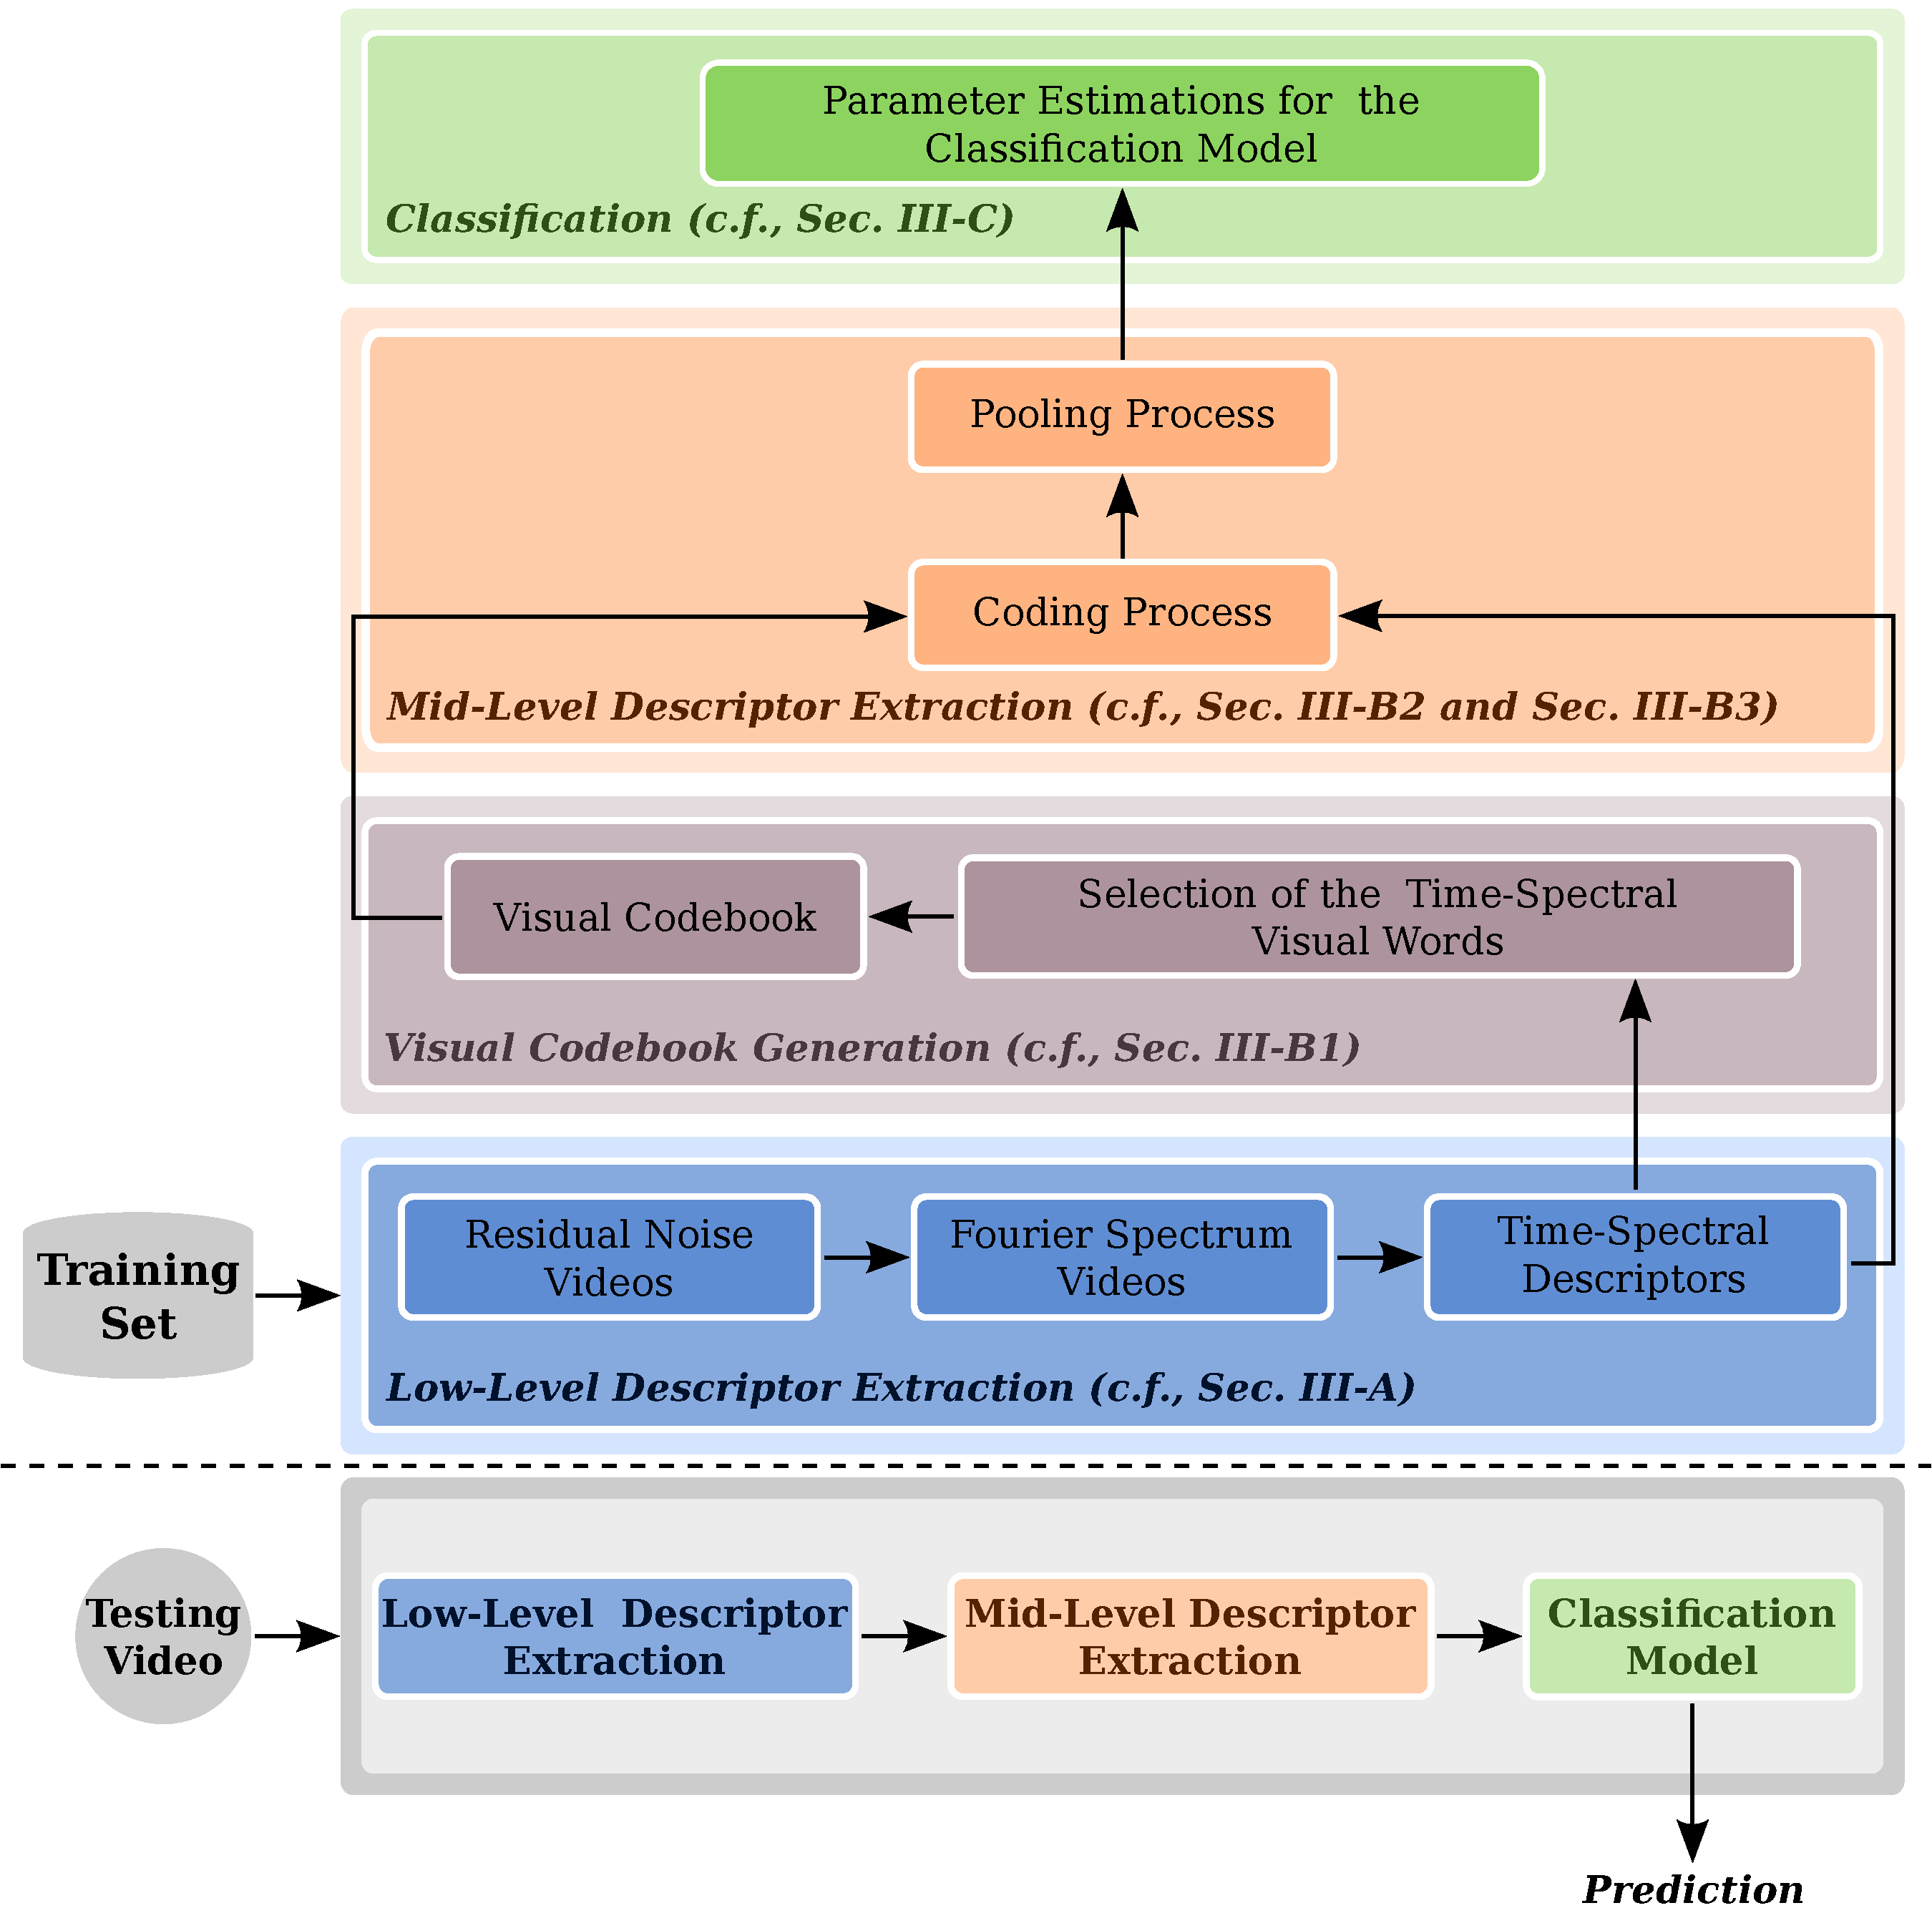
\includegraphics[width=0.45\textwidth]{method_overview_v1.pdf}
\caption{Main steps of the proposed method. Given a training set consisting of valid access and attempted attack videos, and also a testing video, we first extract a noise signature from every training video, generating a \allan{residual noise video}, and calculate its spectrum video. Then, we extract time-spectral descriptors from spectrum videos (low-level representation), which \minor{are used to generate} a visual codebook. With the visual codebook at hand, we transform the low-level descriptors in time-spectral visual word descriptors (mid-level representation). Finally, these mid-level descriptors are used to find parameters of the classification model, which \minor{are employed to predict} whether a given testing video is an attempted attack.}
\label{fig:method_overview}
\end{figure}

\minor{Recent works~\cite{Maatta:IJCB:2011, Pinto:SIBGRAPI:2012, Tan:ECCV:2010} show that noise and artifacts such as blurring effects, printing artifacts, banding effects, and Moir\'{e} patterns are added to the synthetic biometric samples during their manufacture and recapture. In this paper, we propose a spatio-temporal algorithm that captures such effects along time to provide an effective discriminative signature for valid access and spoofing attempts. In summary, the main contributions of this paper are:}
%
\begin{itemize}
	\item a new method for extracting temporal and spectral information from face biometric samples, referred to as time-spectral descriptors;
	\item evaluation of the visual codebook model, also referred to as Bag-of-Visual-Word model, for creating a mid-level representation from time-spectral descriptors, referred to as time-spectral visual words; and
	\item a low-cost solution for spoofing detection, \minor{illustrated in Figure~\ref{fig:method_overview}}, that does not rely on the user interaction or on extra hardware (e.g., infrared, motion or depth sensors) to detect different types of synthetic samples or attacks (e.g., photos, videos and masks) and is amenable to be implemented in computational devices such as PCs, handheld, and embedded systems. 
\end{itemize}

We organize the remaining of this paper as follows. Section~\ref{sec:relatedwork} discusses state-of-the-art methods for face spoofing attack detection. Section~\ref{sec:method} presents our method for spoofing attack detection. Section~\ref{sec:experimentalresults} shows and discusses the experimental protocol and the obtained results. Finally, Section~\ref{sec:conclusions} concludes the paper and discusses possible future work.
 % rereview by Menotti on 1h30
%!TEX root = 2014-TIFS-dl-spoofing.tex
\section{Related Work}
\label{sec:relatedwork}
In this section, we review anti-spoofing related work for iris, face, and fingerprints, our focus in this paper.

\subsection{Iris Spoofing}
Daugman~\cite[Section 8 -- Countermeasures against Subterfuge]{Daugman:1999}\footnote{It also appears in a lecture of Daugman at IBC 2004~\cite{ Daugman:IBC:2004}.} was one of the first authors to discuss the feasibility of some attacks on iris recognition systems. The author proposed the use of Fast Fourier Transform to verify the high frequency spectral magnitude in the frequency domain.

%From the analysis of the iris patterns, it is possible to distinguish a printed iris image from a real one due to the characteristics of the periodic dot printing.

The solutions for iris liveness detection available in the literature range from active solutions relying on  special acquisition hardware~\cite{Lee:LNCS:2005,Pacut:2006,Kanematsu:2007} to software-based solutions relying on texture analysis of the  effects of an attacker using color contact lenses with someone else's pattern printed onto them~\cite{Wei:2008}. Software-based solutions have also explored the effects of cosmetic contact lenses~\cite{Kohli:ICB:2013,Doyle:BTAS:2013,Bowyer:Computer:2014,Yadav:TIFS:2014}; pupil constriction~\cite{Huang:WACV:2013}; and multi biometrics of  electroencephalogram (EEG) and iris together~\cite{Kathikeyan:ICCCA:2012}, among others.

%Nonetheless, in the followings of this subsection, we describe in details those works directly related to the databases we use in this article.

%In \cite{Lee:LNCS:2005}, Lee et al. proposed a new method based on the theoretical positions and distances between the Purkinje image (reflections of objects from the structure of the eye) based on the human eye model by using two alternating collimated \emph{Infra-Red Light Emitting Diode} (IR-LED) requiring special hardware and constrained environment. Experiments using 30 persons (10 without glasses and no contact lens, 10 without glasses and using contact lenses, and with glasses and no contact lens) and 15 counterfeit samples (2D printed iris image, 3D artificial eye and 3D patterned contact lens) were acquired. The real and fake samples where evaluated 10 and 20 times each one, respectively. The obtained results showed impressive results: 0.33 (1/300) false acceptance rate (FAR) and false rejection rate (FRR).

%In \cite{Pacut:2006}, Pacut \& Czajka introduced three liveness detection algorithm based on analysis of image frequency spectrum (FS), controlled light reflection (CLR )from the cornea and pupil dynamics (PD). These methodologies were evaluated using printed fake eye images produced with different printers and printout carries. A small hole is made in place of the pupil, and this trick was enough for fake iris capturing by commercial systems. The experimental results obtained on the evaluation set composed of only 77 pairs of fake and live iris images showed that the CLR and PD methodologies achieves zero error rates and two commercial cameras have achieved $73.1\%$ and $15.6\%$ of FAR for these fake images.

%Kanematsu et al.~\cite{Kanematsu:2007} have proposed a new method by using a variation in the brightness of an iris pattern induced by a pupillary reflex caused by flash-light illumination, and the classification were performed by a decision threshold of $7\%$ brightness variation rate, which is statistically defined by means of mean and standard variation. Experiments were performed using only 5 images by varying the intensity of illumination in several levels. However no effectiveness rates are reported in this work.

%In \cite{Wei:2008}, Wei et al have addressed the problem of iris liveness detection based on three texture measures: iris edges sharpness (ES), iris-texton feature for characterizing the visual primitives of iris texture (IT) and using selected features based on co-occurrence matrix (CM). In special, they use fake iris wearing color contact lens with textures printed onto them. The experiments showed that the ES feature achieved comparable results to the state-of-the-art methods at that time, and the IT and CM measures outperform the state-of-the-art.

Galbally et al.~\cite{Galbally:ICB:2012} investigated 22 image quality measures (e.g., focus, motion, occlusion, and pupil dilation).
The best features are selected through sequential floating feature selection (SFFS)~\cite{Pudil:PRL:1994} to feed a quadratic discriminant classifier. The authors validated the work on the BioSec~\cite{Fierrez-Aguilar:2007,Ruiz-Albacete:BIOID:2008} benchmark. Sequeira et al.~\cite{Sequeira:VISAPP:2014} 
also explored image quality measures~\cite{Galbally:ICB:2012} and three classification techniques validating the work on the BioSec~\cite{Fierrez-Aguilar:2007,Ruiz-Albacete:BIOID:2008} and Clarkson~\cite{LivDet:Iris:2013} benchmarks and introducing the MobBIOfake benchmark comprising 800 iris images from the MobBIO multimodal database~\cite{Sequeira:VISAPP:2014:base}.

Sequeira et al.~\cite{Sequeira:IJCNN:2014} extended upon previous works also exploring quality measures. They first used a feature selection step on the features of the studied methods to obtain the ``best features'' and then used well-known classifiers for the decision-making. In addition, they applied iris segmentation~\cite{Monteiro:CCIS:2014} to obtaining the iris contour and adapted the feature extraction processes to the resulting non-circular iris regions. The validation considered five datasets (BioSec~\cite{Fierrez-Aguilar:2007,Ruiz-Albacete:BIOID:2008}, MobBIOfake~\cite{Sequeira:VISAPP:2014:base}, Warsaw~\cite{Czajka:MMAR:2013}, Clarkson~\cite{LivDet:Iris:2013} and NotreDame~\cite{Doyle:2014:base}.

Textures have also been explored for iris liveness detection. In the recent MobILive\footnote{MobLive 2014, Intl. Joint Conference on Biometrics (IJCB).}~\cite{Sequeira:IJCB:2014} iris spoofing detection competition, the winning team explored three texture descriptors: Local Phase Quantization (LPQ)~\cite{Ojansivu:ISP:2008}, Binary Gabor Pattern~\cite{Zhang:ICIP:2012}, and Local Binary Pattern (LBP)~\cite{Ojala:TPAMI_2002}.

Analyzing printing regularities left in printed irises, Czajka~\cite{Czajka:MMAR:2013} explored some peaks in the frequency spectrum were associated to spoofing attacks. For validation, the authors introduced the Warsaw dataset containing 729 fake images and 1,274 images of real eyes. 
In~\cite{LivDet:Iris:2013}, The First Intl. Iris Liveness Competition in 2013, the Warsaw database was also evaluated, however, the best reported result achieved $11.95\%$ of FRR and $5.25\%$ of FAR by the University of Porto team.

%For localizing the peaks, the author sets up two disjoint frequency windows located under the iris. The window is used to observe the artifacts inserted during printing processing and the second window serves as a reference to the observed disturbances in an amplitude spectrum. Finally, a liveness score is calculated based on information from these two windows. In this dataset, it is claimed that the methodology can be set up to obtain no false alarms ($0\%$ of false rejection rate (FRR)) and $5\%$ of false acceptance rate (FAR). 

%Although not directly related to the datasets in our work, it is worthwhile to describe a recent work of 

Sun et al.~\cite{Sun:TPAMI:2014} recently proposed a general framework for iris image classification based on a Hierarchical Visual Codebook (HVC). The HVC encodes the texture primitives of iris images and is based on two existing bag-of-words models. The method achieved state-of-the-art performance for iris spoofing detection, among other tasks.

%Moreover, the authors also developed an iris image dataset with four types of fake iris patterns (iris texture printed on paper, plastic eyeballs, contact lens and synthetic fake iris images) called CASIA-Iris-Fake. The authros claimed that it is the first dataset comprising a large variety of fake iris patterns allowing an advance on the development of unified countermeasures against spoofing attacks. 

In summary, iris anti-spoofing methods have explored hard-coded features through image-quality metrics, texture patterns, bags-of-visual-words and noise artifacts due to the recapturing process. The performance of such solutions vary significantly from dataset to dataset. Differently, here we propose the automatically extract vision meaningful features directly from the data using deep representations.


\subsection{Face Spoofing}
%Spoofing attack is easily performed against face biometrics systems due to low cost to produce a fake sample. As a matter of fact, there are excellent quality printers and digital cameras at a low price nowadays. In addition, the ease in obtaining facial information of a person through social networks and personal pages contributes for low-cost high-profit attacks.

We can categorize the face anti-spoofing methods into four groups~\cite{Schwartz:IJCB:2011}: user behavior modeling, methods relying on extra devices~\cite{Yi:2014}, methods relying on user cooperation and, finally, data-driven characterization methods. In this section, we review data-driven characterization methods proposed in literature, the focus of our work herein.

M\"{a}\"{a}tt\"{a} et al.~\cite{Maatta:IJCB:2011} used LBP operator for capturing printing artifacts and micro-texture patterns added in the fake biometric samples during acquisition. Schwartz et al.~\cite{Schwartz:IJCB:2011} explored color, texture, and shape of the face region and used them with Partial Least Square (PLS) classifier for deciding whether a biometric sample is fake or not. Both works validated the methods with the Print Attack benchmark~\cite{Anjos:IJCB:2011}. Lee et al.~\cite{Lee:ICASSP:2013} also explored image-based attacks and proposed the frequency entropy analysis for spoofing detection.

%Results of these two techniques were reported in the Competition on Counter Measures to 2D Facial Spoofing Attacks~\cite{Chakka:IJCB:2011}, with a Half Total Error Rate (HTER) of $0.00\%$ and $0.63\%$, respectively, upon the Print Attack database~\cite{Anjos:IJCB:2011}.

% as space is required and this approach does not improved the previously existing one, it was removed
%Inspired on the work of M\"{a}\"{a}tt\"{a} et al.~\cite{Maatta:IJCB:2011}, Chingovska et al.~\cite{Chingovska:BIOSEG:2012} investigated the use of different variations of the LBP method, such as LBP$^{u2}_{3 \times 3}$, tLBP (transitional), dLBP (direction-coded) and mLBP (modified LBP). The feature vectors obtained with these descriptors were classified through $\chi^{2}$ histogram comparison, linear discriminant analysis (LDA) and SVM. However, the method did not outperform the original one~\cite{Maatta:IJCB:2011}. 

Pinto et al.~\cite{Pinto:SIBGRAPI:2012} pioneered research on video-based face spoofing detection. They proposed visual rhythm analysis to capture temporal information on face spoofing attacks.

%Firstly, the face region is isolated and normalized using $z$-score. Thereafter, independent component analysis (ICA) is used to eliminate cross-channel noise caused by interference from the environment. Finally, the authors use the power spectrum and analyze the entropy of the RBG channels individually to further decide upon the attack based on an empirical threshold.

%During a video-based spoofing attack, a noise signature is added to the biometric samples during the recapture of the attack videos and can be used successfully to detect such attacks.

Mask-based face spoofing attacks have also been considered thus far. Erdogmus et al.~\cite{Erdogmus:BIOSIG:2013} dealt with the problem through Gabor wavelets: local Gabor binary pattern histogram sequences~\cite{Zhang:ICCV:2005} and Gabor graphs~\cite{Wiskott:TPAMI:1997} with a Gabor-phase based similarity measure~\cite{Gunther:ICANN:2012}. Erdogmus \& Marcel~\cite{Erdogmus:BTAS:2013} introduced the 3D Mask Attack database (3DMAD), a public available 3D spoofing database, recorded with Microsoft Kinect sensor.

%They also investigate the use of the LBP-based method and reported an HTER of $0.95\%$ and $1.27\%$ using the color and depth images, respectively.

Kose et al.~\cite{Kose:ICASSP:2013} demonstrated that a face verification system is vulnerable to mask-based attacks and, in another work, Kose et al.~\cite{Kose:FG:2013} evaluated the anti-spoofing method proposed by M\"{a}\"{a}tt\"{a} et al.~\cite{Maatta:IJCB:2011} (originally proposed to detect photo-based spoofing attacks). 
Inspired by the work of Tan et al.~\cite{Tan:ECCV:2010}, Kose et al.~\cite{Kose:DSP:2013} evaluated a solution based on reflectance to detect attacks performed with 3D masks. 

%The authors reported an Area Under the Curve (AUC) of $97.0\%$ and a classification accuracy of $94.47\%$ using the non-public available MORPHO database~\cite{Kose:FG:2013}.

Finally, Pereira et al.~\cite{Pereira:ICB:2013} proposed a score-level fusion strategy in order to detect various types of attacks. 
%The authors trained classifiers using different databases and used the $Q$ statistic to evaluate the dependency between classifiers.
%The combination of classifiers that are statistically independent leads to better results. 
In a follow-up work, Pereira et al.~\cite{Pereira:JIVP:2014} proposed an anti-spoofing solution based on the dynamic texture, a spatio-temporal version of the original LBP. Results showed that LBP-based dynamic texture description has a higher effectiveness than the original LBP.

In summary, similarly to iris spoofing detection methods, the available solutions in the literature mostly deal with the face spoofing detection problem through texture patterns (e.g., LBP-like detectors), acquisition telltales (noise), and image quality metrics. Here, we approach the proplem by extracting meaningful features directly from the data regardless of the input type (image, video, or 3D masks).


\subsection{Fingerprint Spoofing}
%There are several approaches for fingerprint spoofing detection. 
We can categorize fingerprint spoofing detection methods roughly into two groups: hardware-based (exploring extra sensors) and software-based solutions (relying only on the information acquired by the standard acquisition sensor of the authentication system)~\cite{Ghiani:ICB:2013}. 

%Methods following the first approach use information provided from additional sensors to gather artifacts that reveal a spoofing attack that are outside of the fingerprint image. Software-based techniques rely only on the information acquired by the standard acquisition sensor of the authentication system.

Galbally et al.~\cite{Galbally:BIDS:2009} proposed a set of feature for fingerprint liveness detection based on quality measures such as ridge strength or directionality, ridge continuity, ridge clarity, and integrity of the ridge-valley structure. The validation considered the three benchmarks used in LivDet 2009 -- Fingerprint competition~\cite{Marcialis:ICIAP:2009} captured with different optical sensors: Biometrika, CrossMatch, and Identix. Later work~\cite{Galbally:FGCS:2012} explored the method in the presence of gummy fingers.

%The authors built a Biometrika.ATVS  set using the Biometrika database from LivDet 2009 -- Fingerprint competition, and obtained results showing that user cooperation may hinder spoofing attacks.}

%The authors reported an average error of $1.83\%$, $11.12\%$, and $6.73\%$ using Biometrika, CrossMatch and Identix sets, respectively. 


Ghiani et al.~\cite{Ghiani:ICPR:2012} explored LPQ~\cite{Ojansivu:ISP:2008}, a method for representing all spectrum characteristics in a compact feature representation form. The validation considered the four benchmarks used in the LivDet 2011 -- Fingerprint competition~\cite{Yambay:ICB:2012}.

%The authors proposed a rotation-invariant version of LPQ, referenced as Rotation Invariant Local Phase Quantization (RILPQ). 

%A combination between proposed LPQ and LBP yielded even better results with a misclassification rate of $9.2\%$ considering the LivDet 2011 -- Fingerprint competition sets.

Gragnaniello et al.~\cite{Gragnaniello:BIOMS:2013} explored the Weber Local Image Descriptor (WLD) for liveness detection, well suited to high-contrast patterns such as the ridges and valleys of fingerprints images. In addition, WLD is robust to noise and illumination changes. The validation considered the LivDet 2009 and LivDet 2011 -- Fingerprint competition datasets.

%The misclassification rates reported were $7.13\%$ and $27.67\%$, respectively. When the proposed method is combined with RILPQ~\cite{Ojansivu:ICPR:2008}, the misclassification rates in both sets reduce to $3.13\%$ and $12.65\%$, respectively.

Jia et al.~\cite{Jia:ICB:2013} proposed a liveness detection scheme based on Multi-scale Block Local Ternary Patterns (MBLTP). 
Differently of the LBP, the Local Ternary Pattern operation is done on the average value of the block instead of the pixels being more robust to noise. 
The validation considered the LivDet 2011 -- Fingerprint competition benchmarks.

Ghiani et al.~\cite{Ghiani:BTAS:2013} explored Binarized Statistical Image Features (BSIF) originally proposed by Kannala et al.~\cite{Kannala:ICPR:2012}. The BSIF was inspired in the LBP and LPQ methods. In contrast to LBP and LPQ approaches, BSIF learns a filter set by using statistics of natural images~\cite{Hyvrinen:NIS:2009}. The validation considered the LivDet 2011 -- Fingerprint competition benchmarks.

Recent results reported in the LivDet 2013 Fingerprint Liveness Detection Competition~\cite{Ghiani:BTAS:2013} show that fingerprint spoofing attack detection task is still an open problem with results still far from a perfect classification rate.

We notice that most of the groups approach the problem with hard-coded features sometimes exploring quality metrics related to the modality (e.g., directionality and ridge strength), general texture patterns (e.g., LBP-, MBLTP-, and LPQ-based methods), and filter learning through natural image statistics. This last approach seems to open a new research trend, which seeks to model the problem learning features directly from the data. We follow this approach in this work, assuming little a priori knowledge about acquisition-level biometric spoofing and exploring deep representations of the data.


%The best classification results among four used datasets were achieved by one team of the University of Naples Federico II and another from the Dermalog Identification Systems. They reported an average accuracy of $86.63\%$ and $84.63\%$, respectively.

\subsection{Multi-modalities}

Recently, Galbally et al.~\cite{Galbally:TIP:2014} proposed a general approach based on 25 image quality features to detect spoofing attempts in face, iris, and fingerprint biometric systems. Our work is similar to theirs in goals, but radically different with respect to the methods.
Instead of relying on prescribed image quality features, we build features that would be hardly thought by a human expert with AO and FO.
Moreover, here we evaluate our systems in more recent and updated benchmarks.


% done! só deixei in [xx] quando era referenciada uma competição.
%\TODO{Algumas vezes usa in [xx] e outras author at al.[xx], acho que poderia padronizar para author et al.[xx], quando possível, por exemplo alguns paragrafos sobre finger printe}
 % order background first?
%!TEX root = 2014-TIFS-dl-spoofing.tex
\section{Benchmarks}
\label{sec:databases}

In this section, we describe the benchmarks (datasets) that we consider in this work. All them are publicly available upon request and suitable for evaluating countermeasure methods to iris, face and fingerprint spoofing attacks. Table~\ref{tab:databases} shows the major features of each one and in the following we describe their details.


\begin{table*}[tb!]
\begin{center}
\caption{Main features of the benchmarks considered herein.}
\label{tab:databases}
%\tiny  \scriptsize \footnotesize \small \normalsize     
\iffinal
%\small
\else
\tiny
\fi
\begin{tabular}{clccrrrcrrrcrrr}
\hline
\multirow{2}{*}{Modality}
& \multirow{2}{*}{Benchmark/Dataset}
                                            & \multirow{2}{*}{Color}
                                                    &      Dimension
                                                                         &\multicolumn{3}{c}{\# Training}
                                                                                               && \multicolumn{3}{c}{\# Testing} 
                                                                                                                     && \multicolumn{3}{c}{\# Development} \\
\cline{5-7}\cline{9-11}\cline{13-15}
&                                            &       & $cols \times rows$ & Live & Fake & Total && Live & Fake & Total && Live & Fake & Total \\
\hline
\hline
\multirow{3}{*}{Iris}
&Warsaw~\cite{Czajka:MMAR:2013}              & No    & $640 \times  480$ &  228 &  203 &   431 &&  624 &  612 &  1236 \\
&Biosec~\cite{Ruiz-Albacete:BIOID:2008}      & No    & $640 \times  480$ &  200 &  200 &   400 &&  600 &  600 &  1200 \\
&MobBIOfake~\cite{Sequeira:VISAPP:2014:base} & Yes   & $250 \times  200$ &  400 &  400 &   800 &&  400 &  400 &   800 \\
\hline
\multirow{2}{*}{Face}
& Replay-Attack~\cite{Chakka:IJCB:2011}      & Yes   & $320 \times  240$ &  600 & 3000 &  3600 && 4000 &  800 &  4800 &&  600 & 3000 & 3600 \\
& 3dMad~\cite{Chingovska:ICB:2013}           & Yes   & $640 \times  480$ &  350 &  350 &   700 &&  250 &  250 &   500 &&  250 &  250 &  500 \\
\hline
\multirow{4}{*}{Fingerprint} 
&Biometrika~\cite{Ghiani:ICB:2013}           & No    & $312 \times  372$ & 1000 & 1000 &  2000 && 1000 & 1000 &  2000 \\
&CrossMatch~\cite{Ghiani:ICB:2013}           & No    & $800 \times  750$ & 1250 & 1000 &  2250 && 1250 & 1000 &  2250 \\
&Italdata~\cite{Ghiani:ICB:2013}             & No    & $640 \times  480$ & 1000 & 1000 &  2000 && 1200 & 1000 &  2000 \\
&Swipe~\cite{Ghiani:ICB:2013}                & No    & $208 \times 1500$ & 1221 &  979 &  2200 && 1153 & 1000 &  2153 \\
\hline

\end{tabular}
\end{center}
\end{table*}

\subsection{Iris Spoofing Benchmarks}

\subsubsection{Biosec} 
This benchmark was created using iris images from $50$ users of the BioSec~\cite{Ruiz-Albacete:BIOID:2008}.
In total, there are $16$ images for each user ($2$ sessions $\times$ $2$ eyes $\times$ $4$ images), totalizing $800$ valid access images. 
To create spoofing attempts, the original images from Biosec were preprocessed to improve quality and printed using an HP Deskjet 970cxi and an HP LaserJet 4200L printers. 
Finally, the iris images were recaptured with the same iris camera used to capture the original images.

\subsubsection{Warsaw} 
This benchmark contains $1274$ images of $237$ volunteers representing valid accesses and $729$ printout images representing spoofing attempts, which were generated by using two printers: (1) a HP LaserJet 1320 used to produce $314$ fake images with $600$ dpi resolution, and (2) a Lexmark C534DN used to produce $415$ fake images with $1200$ dpi resolution. Both real and fake images were captured by an IrisGuard AD100 biometric device.

\subsubsection{MobBIOfake} 
This benchmark contains live iris images and fake printed iris images captured with the same acquisition sensor, i.e., a mobile phone. To generate fake images, the authors first performed a preprocessing in the original images to enhance the contrast. The preprocessed images were then printed with a professional printer on high quality photographic paper.
%Os autores não forneceram mais dados sobre este dataset.


\subsection{Video-based Face Spoofing Benchmarks}

\subsubsection{Replay-Attack} 
This benchmark contains short video recordings of both valid accesses and video-based attacks of $50$ different subjects. 
To generate valid access videos, each person was recorded in two sessions in a controlled and in an adverse environment with a regular webcam.
Then, spoofing attempts were generated using three techniques:
(1)~\emph{print attack}, which presents to the acquisition sensor hard copies of high-resolution digital photographs printed with a Triumph-Adler DCC 2520 color laser printer; 
(2) \emph{mobile attack}, which presents to the acquisition sensor photos and videos taken with an iPhone using the iPhone screen; 
and (3) \emph{high-definition attack}, in which high resolution photos and videos taken with an iPad are presented to the acquisition sensor using the iPad screen.
%In total, there is $200$ valid access videos and $1000$ spoofing attack videos.

\subsubsection{3DMAD} 
This benchmark consists of real videos and fake videos made with people wearing masks. A total of $17$ different subjects were recorded with a Microsoft Kinect sensor, and videos were collected in three sessions. For each session and each person, five videos of $10$ seconds were captured. The 3D masks were produced by \url{ThatsMyFace.com} using one frontal and two profile images of each subject.
All videos were recorded by the same acquisition sensor.
%In total, there are 85 valid access videos and 85 faces. 
%\ToDo{Allan: how many videos? 85 videos de acesso válido e 85 fakes}


\subsection{Fingerprint Spoofing Benchmarks}

\subsubsection{LivDet2013} 
This dataset contains four sets of real and fake fingerprint readings performed in four acquisition sensors: Biometrika FX2000, Italdata ET10, Crossmatch L Scan Guardian, and Swipe.
For a more realistic scenario, fake samples in Biometrika and Italdata were generated without user cooperation, while fake samples in Crossmatch and Swipe were generated with user cooperation. 
Several materials for creating the artificial fingerprints were used, including gelatin, silicone, latex, among others. 
%Both Biometrika and Italdata sets are composed of $1000$ real images and $1000$ fake images. 
%Already, Crossmatch and Swipe sets are composed of $1250$ real images and $1250$ fake images\footnote{those are the figures reported on the public works, but the real number used in this work is slightly different for the Swipe Dataset}.


%%%%%%%%%%%%%%%%%%%%%%%%%%%%%%%%%%%%%%%%%%%%%%%%%%%%%%%%%%%%%

\subsection{Remark}

% The benchmarks described in this section aim at evaluating the proposed method considering a more realistic scenario, given that heterogeneity of the datasets is a challenge, mainly for algorithms based on machine learning, due to difficulty of finding a generalizable model.

Images found in these benchmarks can be observed in Fig.~\ref{fig:datasets} of Section~\ref{sec:experiments}. 
As we can see, variability exists not only across modalities, but also within modalities. Moreover, it is rather unclear what features might discriminate real from spoofed images, which suggests that the use of a methodology able to use data to its maximum advantage might be a promising idea to tackle such set of problems in a principled way.

% Methods developed to work on some database using specific features might not perform well on other databases of the same problem. 
% This hard scenario hints the use of the proposed framework which aims to learn deep representations from the data of each database such that promising effectiveness is expected to be achieved.




% Even considering each modality alone, we have data from many different sensors, which complicates the problem of detecting an attempted attack, and different modes of spoofing attacks, using different types of equipment and procedures. 

% To have an idea of the difficulty of this problem, consider the images depicted in Fig.~\ref{fig:datasets} (linked to Section~\ref{sec:experiments}).
%\TODO{essa referencia de pagina talvez seja perdida na versao final, melhor deixar apenas o numero da figura}. 
%pp.~\pageref{page:fig:datasets}
% Menotti: concordo que a p�gina n�o � o melhor art�fico, mas a figura est� muito longe, por isso usei "linked to Section~\ref{sec:discussion}
% Observe the high variability even within the same modalities. 
%\question{Experiments in this hard scenario hints at the performance of the proposed framework in a more realistic and operational scenario}%
%{Sentenca confusa, nao estah claro qual eh a conclusao que se queria ter com essa sentenca.}. 
%suggestion
% Methods developed to work on some database using specific features might not perform well on other databases of the same problem. 
% This hard scenario hints the use of the proposed framework which aims to learn deep representations from the data of each database such that promising effectiveness is expected to be achieved.

% In the next section, we describe details of our framework for  spoofing attack detection under different modalities. 
% We shall return to the details in such figure when discussing the experimental results. 

%  
\section{Methodology}
\label{sec:methodology}

In this section, we present the methodology for architecture optimization (AO) and filter optimization (FO) as well as details about how benchmark images are preprocessed, how AO and FO are evaluated across the benchmarks, and how these methods are implemented.

\subsection{Architecture Optimization (AO)}
\label{sec:ao}

Our approach for AO builds upon the work of Pinto et al.~\cite{Pinto:2009} and Bergstra et al.~\cite{Bergstra:2013}, i.e., fundamental, feedforward convolutional operations are stacked by means of hyperparameter optimization, leading to effective yet simple convolutional networks that do not require expensive filter optimization and from which prediction is done by linear support vector machines (SVMs).

Operations in convolutional networks can be viewed as linear and non-linear transformations that, when stacked, extract high level representations of the input. Here we use a well-known set of operations called (i) \emph{convolution} with a bank of filters, (ii) rectified linear \emph{activation}, (iii) spatial \emph{pooling}, and (iv) \emph{local normalization}. Appendix~\ref{sec:convnet_ops} provides a detailed definition of these operations.

We denote as \emph{layer} the combination of these four operations in the order that they appear in the left panel of Fig.~\ref{fig:framework}. Local normalization is optional and its use is governed by an additional ``yes/no'' hyperparameter. In fact, there are other six hyperparameters, each of a particular operation, that have to be defined in order to instantiate a layer. They are presented in the lower part of the left panel in Fig.~\ref{fig:framework} and are in accordance to the definitions of Appendix~\ref{sec:convnet_ops}.

Considering one layer and possible values of each hyperparameter, there are over 3,000 possible layer architectures, and this number grows exponentially with the number of layers, which goes up to three in our case (Fig.~\ref{fig:framework} right panel). In addition, there are network-level hyperparameters, such as the size of the input image, that expand possibilities to a myriad potential architectures.
 
 % and emphasize the need to rapidly evaluate candidate architectures.

 % and that we are interested in learning deep representations extracted with the combination of up to three of such layers (Fig.~\ref{fig:framework} right panel), the importance of hyperparameter optimization in this context becomes clear. 

% Considering one layer and possible values of each hyperparameter, there are over 3,000 possible layer architectures. Given that this number grows exponentially with the number of layers and that we are interested in learning deep representations extracted with the combination of up to three of such layers (Fig.~\ref{fig:framework} right panel), the importance of hyperparameter optimization in this context becomes clear. In addition, there are network-level hyperparameters that expand possibilities even more, like the size of the input image, or the depth of the candidate network.


The overall set of possible hyperparameter values is called \emph{search space}, which in this case is discrete and contains variables that are only meaningful in combination with others. For example, hyperparameters of a given layer are just meaningful if the candidate architecture has actually that number of layers.
In spite of the intrinsic difficulty in optimizing architectures in this space, \emph{random search} has played and important role in problems of this type~\cite{Pinto:2009,Bergstra:2012} and it is the strategy of our choice due to its effectiveness and simplicity.

We can see in Fig.~\ref{fig:framework} that a three-layered network has a total of 25 hyperparameters, seven per layer and four at network level. They are all defined in Appendix~\ref{sec:convnet_ops} with the exception of \emph{input size}, which seeks to determine the best size of the image's greatest axis (rows or columns) while keeping its aspect ratio. Concretely, random search in this paper can be described as follows:

\begin{enumerate}
\item Randomly --- and uniformly, in our case --- sample values from the hyperparameter \emph{search space};
\item Extract features from real and fake training images with the candidate architecture;
\item Evaluate the architecture according to an \emph{optimization objective} based on linear SVM scores;
\item Repeat steps 1--3 until a \emph{termination criterion} is met;
\item Return the best found convolutional architecture.
\\
\end{enumerate}



\begin{figure}
\begin{center}
 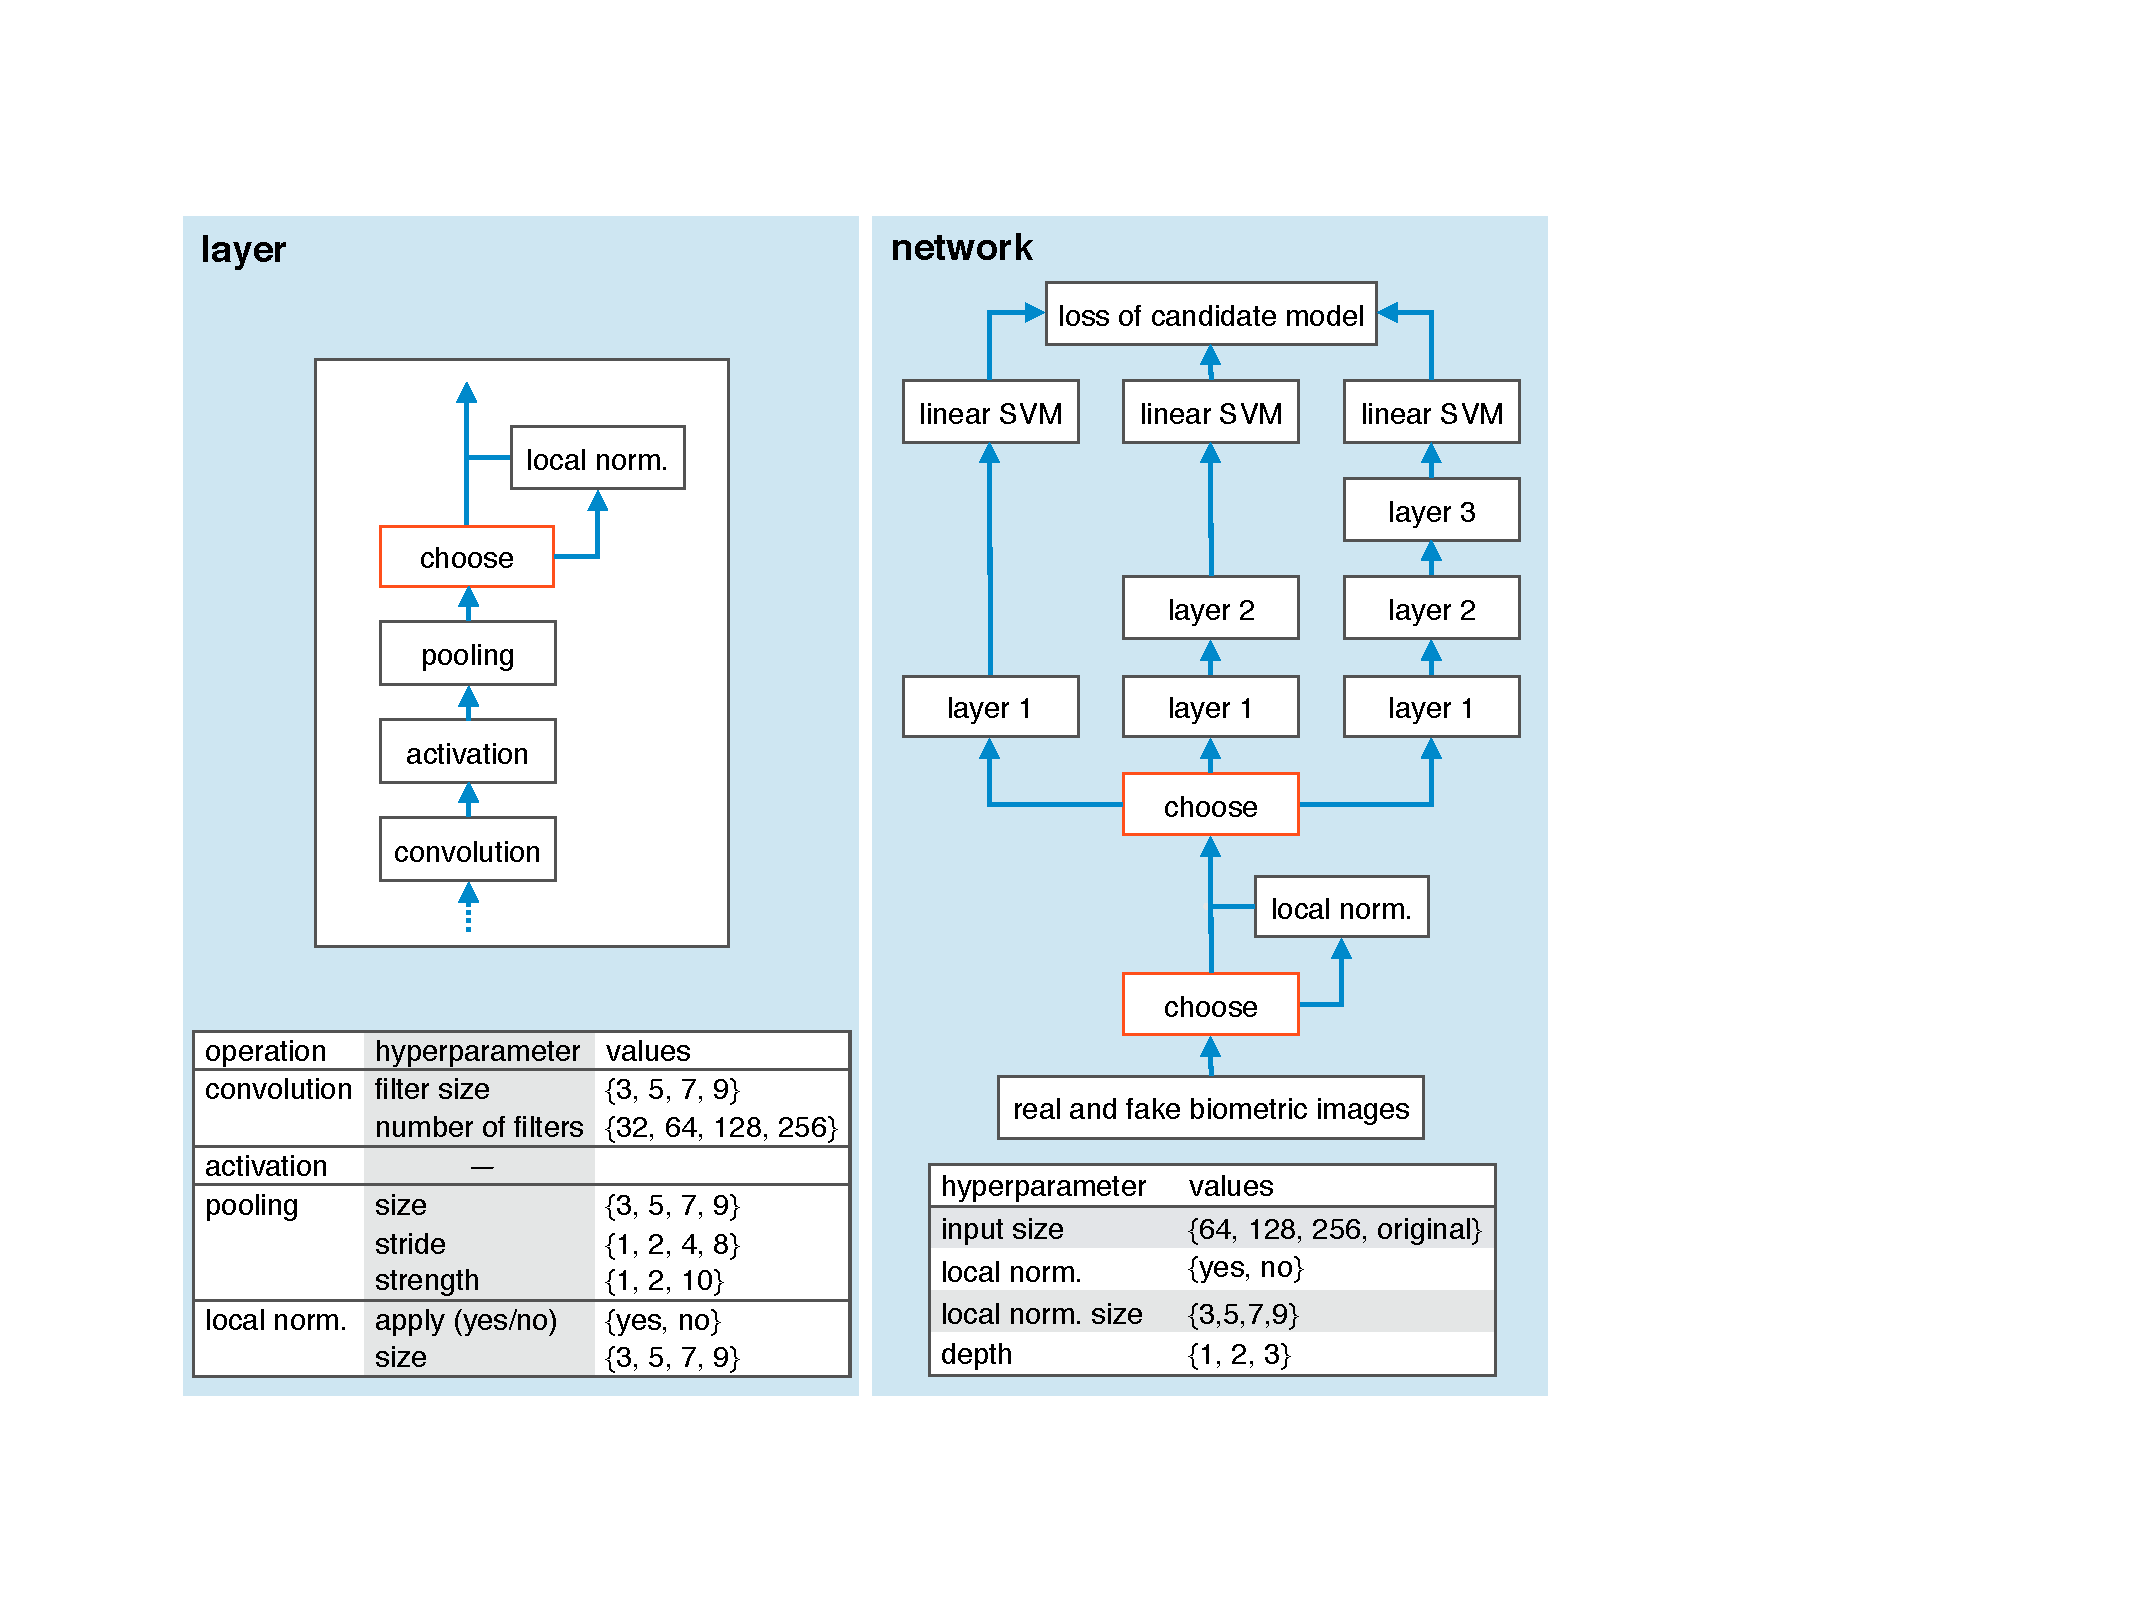
\includegraphics[width=1.0\linewidth]{hp-schema.pdf}
 \caption{Schematic diagram for architecture optimization (AO) illustrating how operations are stacked in a layer (left) and how the network is instantiated and evaluated according to possible hyperparameter values (right). Note that a three-layered convolutional network of this type has a total of 25 hyperparameters governing both its architecture and its overall behaviour through a particular instance of stacked operations.}
 \label{fig:framework}
\end{center}
\end{figure}


Even though there are billions of possible networks in the search space (Fig.~\ref{fig:framework}), it is important to remark that not all candidate networks are valid. For example, a large number of candidate architectures (i.e., points in the search space) would produce representations with spatial resolution smaller than one pixel. Hence, they are naturally unfeasible.
Additionally, in order to avoid very large representations, we discard in advance candidate architectures whose intermediate layers produce representations of over 600K elements or whose output representation has over 30K elements.

% Filter optimization is of paramount importance in convolutional networks and 

Filter weights are randomly generated for AO. This strategy has been successfully used in the vision literature~\cite{Pinto:2009,Saxe:2011,Pinto:2011b,Jarrett:2009} and is essential to make AO practical, avoiding the expensive filter optimization (FO) part in the evaluation of candidate architectures. We sample weights from a uniform distribution $U(0,1)$ and normalize the filters to zero mean and unit norm in order to ensure that they are spread over the unit sphere. When coupled with rectified linear activation (Appendix~\ref{sec:convnet_ops}), this sampling enforces sparsity in the network by discarding about $50$\% of the expected filter responses, thereby improving the overall robustness of the feature extraction.

A candidate architecture is evaluated by first extracting deep representations from real and fake images and later training hard-margin linear SVMs ($C$=$10^5$) on these representations.
We observed that the sensitivity of the performance measure was saturating with traditional 10-fold cross validation (CV) in some benchmarks. Therefore, we opted for a different validation strategy. Instead of training on nine folds and validating on one, we train on one fold and validate on nine. Precisely, the \emph{optimization objective} is the mean detection accuracy obtained from this adapted cross-validation scheme, which is maximized during the optimization.

For generating the 10 folds, we took special care in putting all samples of an individual in the same fold to enforce robustness to cross-individual spoofing detection in the optimized architectures.
Moreover, in benchmarks where we have more than one attack type (e.g., Replay-Attack and LivDet2013, see Section~\ref{sec:databases}), we evenly distributed samples of each attack type across all folds in order to enforce that candidate architectures are also robust to different types of attack.

Finally, the \emph{termination criterion} of our AO procedure simply consists of counting the number of valid candidate architectures and stopping the optimization when this number reaches 2,000.


\subsection{Filter Optimization (FO)}
\label{sec:fo}

\begin{figure}
\begin{center}
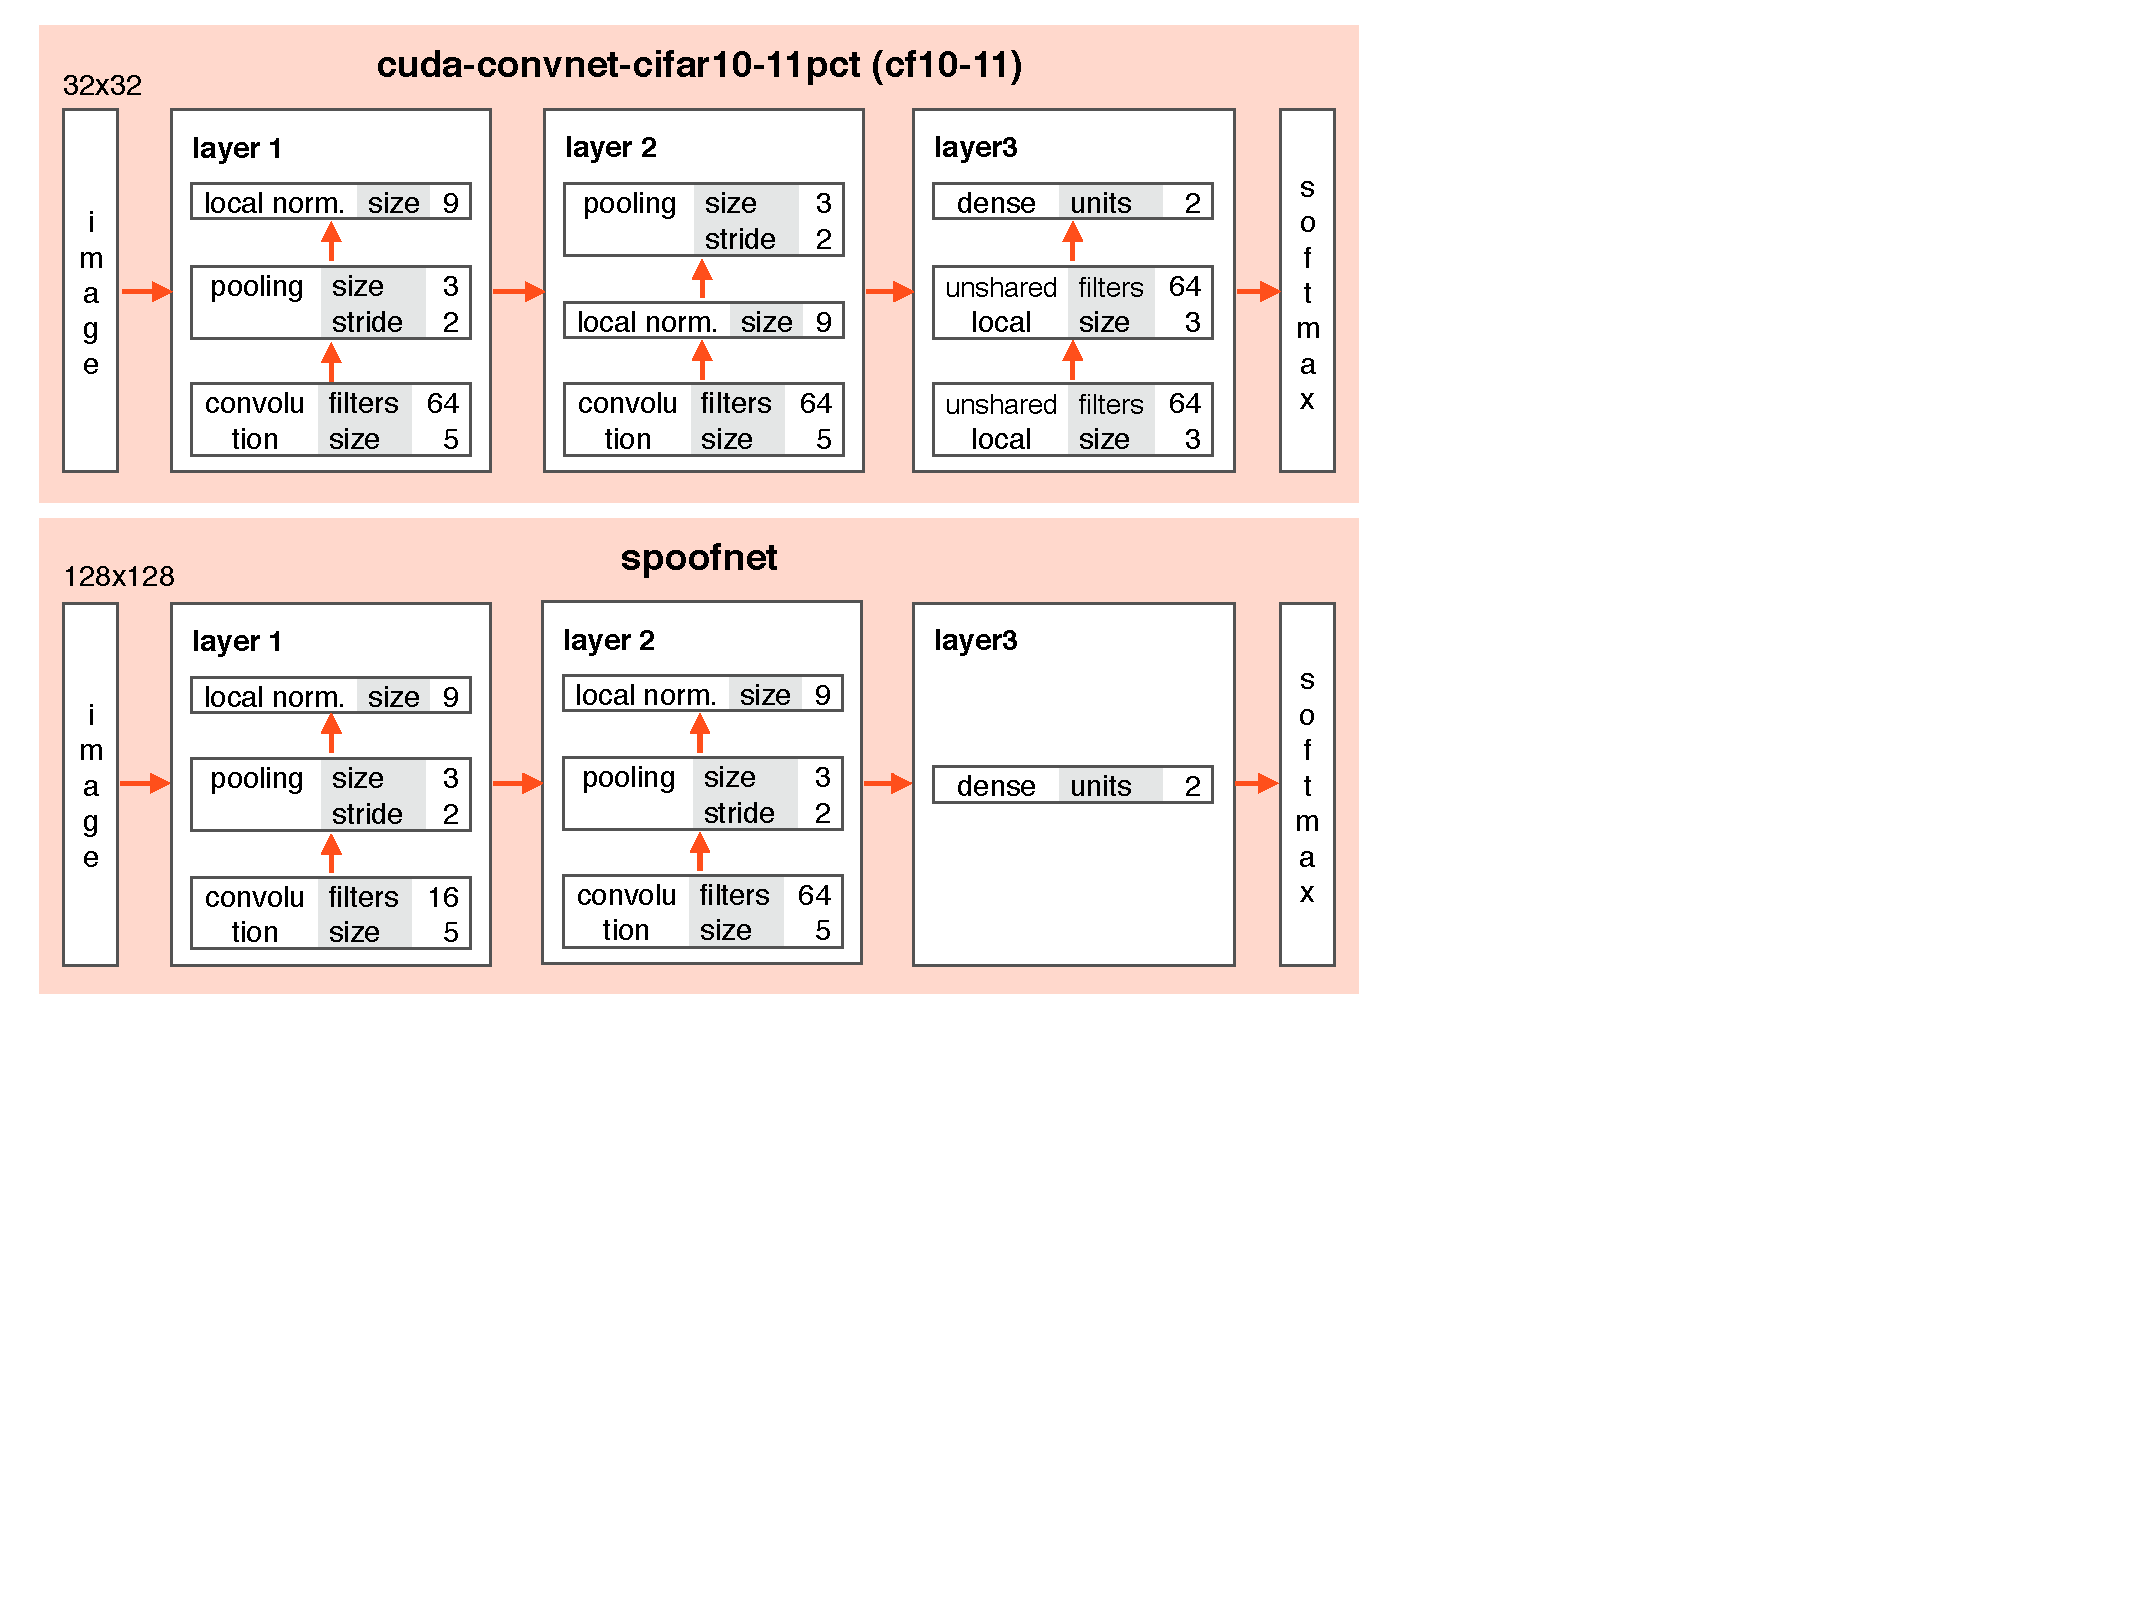
\includegraphics[width=1.0\linewidth]{cuda-convnet.pdf}
\caption{
Architecture of convolutional network found in the Cuda-convnet library~\cite{Krizhevsky:cuda-convnet:2012} and here used as reference for filter optimization (\emph{cf10-11}, top). Proposed network architecture extending upon~\emph{cf10-11} to better suiting spoofing detection problems (\emph{spoofnet}, bottom). Both architectures are typical examples where domain knowledge has been incorporated for increased performance.
}
\label{fig:cudaconvnet}
\end{center}
\end{figure}

We now turn our attention to a different approach for tackling the problem. Instead of optimizing the architecture, we explore the filter weights and how to learn them for better characterizing real and fake samples. Our approach for FO is at the origins of convolutional networks and consists of learning filter weights via the well-known back-propagation algorithm~\cite{LeCun:1998}. Indeed, due to a refined understanding of the optimization process and the availability of plenty of data and processing power, back-propagation has been the gold standard method in deep networks for computer vision in the last years~\cite{Krizhevsky:2012,Simonyan:2014,Zeiler:2014}.

For optimizing filters, we need to have an already defined architecture. We start optimizing filters with a standard public convolutional network and training procedure. This network is available in the Cuda-convnet library~\cite{Krizhevsky:cuda-convnet:2012} and is currently one of the best performing architectures in CIFAR-10,\footnote{\url{http://www.cs.toronto.edu/~kriz/cifar.html}} a popular computer vision benchmark in which such network achieves 11\% of classification error. Hereinafter, we call this network \emph{cuda-convnet-cifar10-11pct}, or simply \emph{cf10-11}.

Fig.~\ref{fig:cudaconvnet} depicts the architecture of \emph{cf10-11} in the top panel and is a typical example where domain knowledge has been incorporated for increased performance. We can see it as a three-layered network in which the first two layers are convolutional, with operations similar to the operations used in architecture optimization (AO). In the third layer, \emph{cf10-11} has two sublayers of unshared local filtering and a final fully-connected sublayer on top of which softmax regression is performed. A detailed explanation of the operations in \emph{cf10-11} can be found in~\cite{Krizhevsky:cuda-convnet:2012}.

In order to train~\emph{cf10-11} in a given benchmark, we split the training images into four batches observing the same balance of real and fake images. After that, we follow a procedure similar to the original\footnote{\url{https://code.google.com/p/cuda-convnet/wiki/Methodology}.} for training~\emph{cf10-11} in all benchmarks, which can be described as follows:

\begin{enumerate}
\item For 100 epochs, train the network with a learning rate of $10^{-3}$ by considering the first three batches for training and the fourth batch for validation;
\item For another 40 epochs, resume training now considering all four batches for training;
\item Reduce the learning rate by a factor of 10, and train the network for another 10 epochs;
\item Reduce the learning rate by another factor of 10, and train the network for another 10 epochs.
\\
\end{enumerate}

% Once~\emph{cf10-11} is trained in a given benchmark, prediction on test samples is performed by softmax 
% The network learned after this process is the one used to evaluate the benchmarks.

After evaluating filter learning on the \emph{cf10-11} architecture, we also wondered how filter learning could benefit from an optimized architecture incorporating domain-knowledge of the problem. Therefore, extending upon the knowledge obtained with AO as well as with training~\emph{cf10-11} in the benchmarks, we derived a new architecture for spoofing detection that we call~\emph{spoofnet}. Fig.~\ref{fig:cudaconvnet} illustrates this architecture in the bottom panel and has three key differences as compared to~\emph{cf10-11}. First, it has 16 filters in the first layer instead of 64. Second, operations in the second layer are stacked in the same order that we used when optimizing architectures (AO). Third, we removed the two unshared local filtering operations in the third layer, as they seem inappropriate in a problem where object structure is irrelevant.

These three modifications considerably dropped the number of weights in the network and this, in turn, allowed us to increase of size of the input images from $32\times32$ to $128\times128$. This is the fourth and last modification in~\emph{spoofnet}, and we believe that it might enable the network to be more sensitive to subtle local patterns in the images.

In order to train~\emph{spoofnet}, the same procedure used to train~\emph{cf10-11} is considered except for the initial learning rate, which is made $10^{-4}$, and for the number of epochs in each step, which is doubled. These modifications were made because of the decreased learning capacity of the network.
% However, given that~\emph{spoofnet} is much faster than~\emph{cf10-11} to process images, the overall training time was not increased.

% For the extended architecture we proposed here, we have developed a slightly different training methodology that the one used for the Krizhevsky \emph{et al.}'s model.
% Indeed, we increase by two the number of training epochs in the three phases described above adding up 320 epochs, since we reduce the number of filter in the first convolutional layer.
% Moreover, we setup the starting learning rate equal to $10^{-4}$, instead of $10^{-3}$ as done in Krizhevsky's methodology.


% We also propose an extended version of Alex's architecture, which can be seen as a reduced one to the complexity of spoofing problem.
% Indeed, we: 1) use only 16 filters in the first convolutional layer; 2) remove the third layer, the locally-connected layer. 
% Moreover $128 \times 128 \times C$ image pixels are used as input for this extended version.
% These modifications made the evaluation time for the extended network at least twice faster.


% The domain knowledge convolution network chosen to be used here for filter learning via backpropagation is the one used in~\cite{Krizhevsky:2012} which achieves accuracy near $90\%$ on CIFAR-10 dataset. 

% In the following we describe in details these architectures, their training methodologies together with the data preparation for and how data augmentation is employed to boost the learning processing.

% More specifically Krizhevsky \emph{et al.}'s (or simply Alex) architecture~\cite{Krizhevsky:2012} can be seen as composed of four layers. 
% In the first one, convolutional operation with 64 filters of $5\times 5$, followed by a $3\times 3$ max-pooling operation with stride 2, and $9 \times 9$ local response/contrast normalization. 
% In the second layer, convolutional operation with 64 filters of $3 \times 3$, followed by $9\times 9$ local response/contrast normalization and then $3\times 3$ max-pooling operation with stride 3.
% In the third layer, we have two locally-connected operations with unshared weight, using 64 and 32 filters of $3\times 3$, respectively.
% The final layer, which can be seen as the classification one, is composed of a fully connected operation to two neurons attached to softmax operations, which can be interpreted as probabilities, where the backpropation starts the learning task with target classes. For such, an objective function should be defined. In this case a (multinomial) logistic regression objective one.
% This network can also be seen as being composed of 11 layers, if each operation is considered as a layer.

% The input for this network uses $32 \times 32 \times c$ image pixels - the standard size of CIFAR-10 dataset, where $c$ stands for the number of channels in the images of each benchmark. 
% But here we adopt $c=1$ for the benchmarks using grayscale images, and keep $c=3$ when color images are available.

Finally, in order to reduce overfitting, data augmentation is used for training both networks according to the procedure of~\cite{Krizhevsky:2012}. For \emph{cf10-11}, five $24\times24$ image patches are cropped out from the $32\times32$ input images. These patches correspond to the four corners and central region of the original image, and their horizontal reflections are also considered. Therefore, ten training samples are generated from a single image. For \emph{spoofnet}, the procedure is the same except for the fact that input images have $128\times128$ pixels and cropped regions are of $112\times112$ pixels. During prediction, just the central region of the test image is considered.


\subsection{Elementary Preprocessing}
\label{sec:preproc}

A few basic preprocessing operations were executed on face and fingerprint images in order to properly learn representations for these benchmarks. 
This preprocessing led to images with sizes as presented in Table~\ref{tab:databases:experiments} and are described in the next two sections.

\begin{table}[tb!]
\begin{center}
\caption{Input image dimensionality after basic preprocessing on face and fingerprint images (highlighted). See Section~\ref{sec:preproc} for details.}
\label{tab:databases:experiments}
\begin{tabular}{clc}
\hline
\multirow{2}{*}{Modality}
& \multirow{2}{*}{Benchmark}
                                             & Dimensions \\
&                                            & $columns \times rows$ \\
\hline
\hline
\multirow{3}{*}{Iris}
&Warsaw~\cite{Czajka:MMAR:2013}              & $640 \times  480$ \\
&Biosec~\cite{Ruiz-Albacete:BIOID:2008}      & $640 \times  480$ \\
&MobBIOfake~\cite{Sequeira:VISAPP:2014:base} & $250 \times  200$ \\
\hline
\multirow{2}{*}{Face}
& Replay-Attack~\cite{Chakka:IJCB:2011}      & $\mathbf{200 \times  200}$ \\
& 3DMAD~\cite{Chingovska:ICB:2013}           & $\mathbf{200 \times  200}$ \\
\hline
\multirow{4}{*}{Fingerprint} 
&Biometrika~\cite{Ghiani:ICB:2013}           & $\mathbf{312 \times  372}$ \\
&CrossMatch~\cite{Ghiani:ICB:2013}           & $\mathbf{480 \times  675}$ \\
&Italdata~\cite{Ghiani:ICB:2013}             & $\mathbf{384 \times  432}$ \\
&Swipe~\cite{Ghiani:ICB:2013}                & $\mathbf{187 \times  962}$ \\
\hline

\end{tabular}
\end{center}
\end{table}

\subsubsection{Face Images}

Given that the face benchmarks considered in this work are video-based, we first evenly subsample 10 frames from each input video. Then, we detect the face position using Viola \& Jones~\cite{Viola:IJCV:2001} and crop a region of $200 \times 200$ pixels centered at the detected window.

\subsubsection{Fingerprint Images}
Given the diverse nature of images captured from different sensors, here the preprocessing is defined according to the sensor type.
\begin{enumerate}[(a)]
\item \emph{Biometrika}: we cropped the central region of size in columns and rows corresponding to 70\% of the original image dimensions. 
\item \emph{Italdata} and \emph{CrossMatch}: we cropped the central region of size in columns and rows respectively corresponding to 60\% and 90\% of the original image columns and rows.
\item \emph{Swipe}: As the images acquired by this sensor contain a variable number of blank rows at the bottom, the average number of non-blank rows $M$ was first calculated from the training images.
Then, in order to obtain images of a common size with non-blank rows, we removed their blank rows at the bottom and rescaled them to $M$ rows. Finally, we cropped the central region corresponding to 90\% of original image columns and $M$ rows.
\end{enumerate}

The rationale for these operations is based on the observation that fingerprint images in LivDet2013 tend to have a large portion of background content and therefore we try to discard such information that could otherwise mislead the representation learning process.
The percentage of cropped columns and rows differs among sensors because they capture images of different sizes with different amounts of background.

For architecture optimization (AO), the decision to use image color information was made according to 10-fold validation (see Section~\ref{sec:ao}), while for filter optimization (FO), color information was considered whenever available for a better approximation with the standard cf10-11 architecture. Finally, images were resized to $32\times32$ or $128\times128$ to be taken as input for the cf10-11 and spoofnet architectures, respectively. 

\subsection{Evaluation Protocol}
\label{sec:evalprot}

For each benchmark, we learn deep representations from their training images according to the methodology described in Section~\ref{sec:ao} for architecture optimization (AO) and in Section~\ref{sec:fo} for filter optimization (FO).
We follow the standard evaluation protocol of all benchmarks and evaluate the methods in terms of detection accuracy (ACC) and half total error rate (HTER), as these are the metrics used to assess progress in the set of benchmarks considered herein. Precisely, for a given benchmark and convolutional network already trained, results are obtained by:

\begin{enumerate}
\item Retrieving prediction scores from the testing samples;
\item Calculating a threshold $\tau$ above which samples are predicted as attacks;
\item Computing ACC and/or HTER using $\tau$ and test predictions.
\end{enumerate}

The way that $\tau$ is calculated differs depending on whether the benchmark has a development set or not (Table~\ref{tab:databases}). Both face benchmarks have such a set and, in this case, we simply obtain $\tau$ from the predictions of the samples in this set. 
Iris and fingerprint benchmarks have no such a set, therefore $\tau$ is calculated depending on whether the convolutional network was learned with AO or FO.

In case of AO, we calculate $\tau$ by joining the predictions obtained from 10-fold validation (see Section~\ref{sec:ao}) in a single set of positive and negative scores, and $\tau$ is computed as the point that lead to an equal error rate (EER) on the score distribution under consideration. 
In case of FO, scores are probabilities and we assume $\tau=0.5$. ACC and HTER are then trivially computed with $\tau$ on the testing set.

It is worth noting that the Warsaw iris benchmark provides a supplementary testing set that here we merge with the original testing set in order to replicate the protocol of~\cite{LivDet:Iris:2013}.
Moreover, given face benchmarks are video-based and that in our methodology we treat them as images (Section~\ref{sec:preproc}),
we perform a score-level fusion of the samples from the same video according to the max rule~\cite{Ross:HM:2006}. This fusion is done before calculating $\tau$.


\subsection{Implementation}
\label{sec:implementationdetais}

Our implementation for architecture optimization (AO) is based on Hyperopt-convnet~\cite{Bergstra:2013b} which in turn is based on Theano~\cite{Bergstra:SCIPY:2010}.
LibSVM~\cite{Chang:2011} is used for learning the linear classifiers via Scikit-learn.\footnote{http://scikit-learn.org}
The code for feature extraction runs on GPUs due to Theano and the remaining part is multithreaded and runs on CPUs.
We extended Hyperopt-convnet in order to consider the operations and hyperparameters as described in Appendix~\ref{sec:convnet_ops} and Section~\ref{sec:ao} and we will make the source code freely available in~\cite{Chiachia:2014b}.
Running times are reported with this software stack and are computed in an Intel i7 @3.5GHz with a Tesla K40 that, on average, takes less than one day to optimize an architecture --- i.e., to probe 2,000 candidate architectures --- for a given benchmark.

As for filter optimization (FO), Cuda-convnet~\cite{Krizhevsky:cuda-convnet:2012} is used. This library has an extremely efficient implementation to train convolutional networks via back-propagation on NVIDIA GPUs. 
Moreover, it provides us with the cf10-11 convolutional architecture taken in this work as reference for FO.

\section{Experiments and Results}\label{sec:experimentalresults}
In this section, we present and discuss the experimental results and the validation of the proposed method. Section~\ref{subsec:Database} shows details of the datasets used in the experiments while Section~\ref{subsec:Protocol} describes the experimental protocols employed in this work. Section~\ref{sec:setup} shows the experimental setup of the proposed method regarding its parameters. The experiments in Section~\ref{subsec:analysis} aim at validating our method and choosing its best parameter setup. In addition, Section~\ref{subsec:analysis} addresses important questions regarding the low- and mid-level descriptor extraction procedures: {(1) the best characteristic extracted from Fourier spectrum (e.g., magnitude or phase spectrum); (2) the best measure for spectrum summarization (e.g., energy, entropy, correlation, mutual information, etc);} and (3) the visual codebook size most appropriate for the problem; among others. The remaining subsections compare the proposed method with the best methods reported in the literature including a challenging cross-dataset protocol, whereby we train our method using a dataset and test it with another dataset.

\subsection{Datasets}
\label{subsec:Database}
In this work, we consider four datasets:
%
\begin{itemize}
\item \textbf{Replay-Attack Dataset~\cite{Chingovska:BIOSEG:2012}}: This dataset comprises videos of valid accesses and attacks of $50$ identities. The videos were generated with a webcam with a resolution of $320 \times 240$ pixels and $25$ frames per second (fps). {This dataset contains $200$ valid access videos, $200$ print-based attacks, $400$ mobile-based attacks using an iPhone, and $400$ high-definition attacks using an iPad screen with $1,024 \times 768$ pixel resolution.}

\item \textbf{CASIA Face Anti-Spoofing Dataset~\cite{Zhang:ICB:2012}}: This dataset contains videos of valid accesses and attacks of $50$ identities and considers different types of attacks such as warped photo attacks and cut photo attacks, besides the photos and video attacks. It also considers attacks performed with different image/video quality: 
{(1)~low-quality videos captured by a long-time-used USB camera with $480 \times 640$ pixel resolution; (2) normal-quality videos captured with a new USB camera with $480 \times 640$ pixel resolution; and (3) high-quality videos captured with a Sony NEX-5 camera with $1,920 \times 1,080$ pixel resolution.} In total, it comprises $150$ valid access videos and $450$ video spoofing attacks.

\item \textbf{UVAD Dataset~\cite{Pinto:Unicamp:2013, Pinto:TIFS:2015}\footnote{This dataset is freely available through FigShare \allan{(http://figshare.com/articles/visualrhythm\_antispoofing/1295453)}.}}: This dataset contains valid access and attempted attack videos of {$404$ different people}, all created at Full HD quality, $30$ fps, and nine seconds long. It contains {$16,268$ attempted attack videos and $808$ valid access videos}. {Seven different display devices} were used to simulate the attempted attacks performed upon three acquisition sensors of different manufacturers: {a 9.1 megapixel (MP) Sony CyberShot DSC-HX1, a 10.0-MP Canon PowerShot SX1 IS, a 10.3-MP Nikon Coolpix P100, a 14.0-MP Kodak Z981, a 14.0-MP Olympus SP 800UZ, and a 12.1-MP Panasonic FZ35 digital camera. Figs.~\ref{fig:exemplosVideosValidos} and~\ref{fig:exemplosVideosAtaque} illustrate some examples of this dataset.}
%
\begin{figure*}[!htb]
\centering
\begin{tabular}{c}
	\includegraphics*[width=0.12\textwidth]{facesReais/MAH00938.PNG}
	\includegraphics*[width=0.12\textwidth]{facesReais/MAH01011.PNG}
	\includegraphics*[width=0.12\textwidth]{facesReais/MAH01205.PNG}
	\includegraphics*[width=0.12\textwidth]{facesReais/MAH01241.PNG}
	\includegraphics*[width=0.12\textwidth]{facesReais/MAH01502.PNG}
\end{tabular}
\caption{Examples of valid access video frames for outdoor (first and second images on the left) and indoor (three images on the right) scenes.}
\label{fig:exemplosVideosValidos}
\end{figure*}
%
\begin{figure*}[!htb]
\centering
\begin{tabular}{c}
	\includegraphics*[width=0.12\textwidth]{facesFakes/MAH00938.PNG}
	\includegraphics*[width=0.12\textwidth]{facesFakes/MAH01011.PNG}
	\includegraphics*[width=0.12\textwidth, height=0.082\textheight]{facesFakes/MAH01205.PNG}
	\includegraphics*[width=0.12\textwidth, height=0.082\textheight]{facesFakes/MAH01241.PNG}
	\includegraphics*[width=0.12\textwidth, height=0.082\textheight]{facesFakes/MAH01502.PNG}
\end{tabular}
\caption{Examples of attempted attack video frames for outdoor (first and second images on the left) and indoor (three images on the right) scenes using Sony (first and second columns), Canon (third and fourth columns) and Nikon (last column) cameras.}
\label{fig:exemplosVideosAtaque}
\end{figure*}

\item \textbf{3DMAD Dataset~\cite{Erdogmus:BTAS:2013}}: This dataset comprises valid access and mask attack videos of $17$ different subjects, whose faces were recorded by a Microsoft Kinect sensor. To build a synthetic biometric sample, the authors used frontal and profile face images to make the facial reconstruction. Afterwards, the authors used a 3D printer to build a mask containing facial information of the target person. Spoofing attack simulations were performed by presenting the 3D masks to the same Microsoft Kinect sensor. In total, the authors generated $85$ valid access videos and $85$ attempted attack videos.
\end{itemize}

\subsection{Experimental Protocol}
\label{subsec:Protocol}
We use \redmark{two measures for performance evaluation}: the area under the curve (AUC) and the half total error rate (HTER). \minor{While the former} quantifies the overall ability of a classifier to discriminate between attempted attacks and valid accesses, \minor{the latter} combines the false acceptance rate (FAR) and false rejection rate (FRR) in a specific operating point of the ROC curve into a single measure. HTER is commonly calculated in the operating point in which the FAR is equal to the FRR, known as the Equal Error Rate (EER). \redmark{We use the freely available toolbox Bob~\cite{Anjos:ACMMM:2012} to calculate the AUC and HTER values. Finally,} the employed evaluation protocols follow the ones proposed by the authors of the Replay-Attack, \allan{CASIA,} UVAD and 3DMAD datasets. The source code of all proposed methods are freely available.\footnote{{The source code is freely available for scientific purposes on GitHub \allan{(https://github.com/allansp84/spectralcubes)}, along with this article.}}

\subsubsection{Protocol I} In this experimental protocol, we use the Replay-Attack dataset, which is divided into three subsets: a training set with $300$ attack videos and $60$ valid videos; a development set with $300$ attack videos and $60$ valid access videos; and a test set with $400$ attempted attack videos and $80$ valid access videos. \minor{The training set is used to fit a classification model, the development set to find the EER, whereas the test set is used to report the final error rates.}

\subsubsection{Protocol II} \minor{In this protocol, we use CASIA dataset, divided into two disjoint subsets: training and test sets. \allan{Due to the absence of a development set to estimate a threshold to be applied in the test set and afterwards to calculate the HTER, the official protocol of this dataset recommends to use the training set to build a classifier and then use the test set to report the EER value. To report the results in terms of HTER, the original training set was divided into two subsets, named as training and development sets, in the proportion of $80\%$ and $20\%$, respectively. We use the new training set to find the classification model and the development set to estimate the threshold that gives us the EER, whereas the official test set is used to report the final results in terms of HTER.}
}


%\subsubsection{Protocol II} This is a protocol similar to Protocol I except that we use CASIA dataset instead of Replay-Attack. This dataset is already divided into training and test sets. We split the training into 80\% for actual training and 20\% for development (parameter {optimization}). Finally, the {official} test set was used as the test set.

%\subsubsection{Protocol III} In this protocol, we use the UVAD dataset, which contains one subset with $304$ valid access videos and three subsets, each one with $2,343$ attempted attack videos. Each subset contains attempted attack videos that were generated through spoofing attacks performed in a face biometric system equipped with one of three sensors: Sony, Canon, or Nikon. We use a cross-dataset evaluation protocol here in which we train the classification model with the Replay-Attack dataset and we use UVAD valid access and attempted attack videos to perform the test.

\subsubsection{Protocol III} \minor{In this protocol, we use the UVAD dataset, which contains six subsets comprising valid access and attempted attack videos. Each subset considers attacks against one acquisition sensor: Sony, Kodak, Olympus, Nikon, Canon and Panasonic. Here, we train a classifier using the sensors Sony, Kodak and Olympus, and we test it with videos (valid access and attempted attacks) from three other different manufacturers: Nikon, Canon and Panasonic.}

\subsubsection{Protocol IV} \minor{Here, we use the 3DMAD dataset to evaluate spoofing detection of attacks using 3D masks. The dataset contains $85$ RGB videos that represent valid access and $85$ RGB videos that represent attempted spoofing attacks. As this dataset does not contain explicit subsets, we randomly partitioned the data into three subsets: training, development and testing, and we use Protocol I for testing.}

\subsection{Method Parameterization}\label{subsec:setup}
\label{sec:setup}
For reproducibility purposes, \minor{this section discuss} the parameters whose values are constant in the setup of our method. 

We extract the \redmark{noise signature} from RGB videos using a Gaussian filter with~$\mu = 0$,~$\sigma = 0.5$, and kernel size~$ 3 \times 3$ (Eq.~\ref{eq:ruido}). These values were obtained empirically in~\cite{Pinto:SIBGRAPI:2012}. Next, we extract cuboids of size $32 \times 32 \times 8$ from the Fourier spectrum videos (Eqs.~\ref{eq:mag_spectrum} and~\ref{eq:phase_spectrum}), whose spatio-temporal location is \redmark{chosen randomly based on} a uniform distribution. 

The use of spatial measures produces {low-level $8$-dimensional descriptors} per channel, whereas the use of spatio-temporal measures produces low-level $7$-dimensional descriptors per channel, which gives us a final low-level descriptor of $24$-dimensional and $21$-dimensional, respectively. Finally, the number of cubes extracted from videos is determined by dividing the volume of the video with respect to the cube.

\redmark{Regarding the mid-level descriptors}, the only parameters with constant values are the ones that define the Gaussian kernel used in the soft-assignment coding technique, whose values are~$\mu = 0$ and~$\sigma = 0.04$. Finally, the SVM parameters are found through grid search in  the training data.

\subsection{Experimental Design and Analysis}\label{subsec:analysis}

\begin{table*}
\begin{center}
\begin{footnotesize}
\footnotesize
\caption{{After the statistical analysis, we have found that the factors highlighted with $\dagger$ are the ones that did not present statistical significance when configuring our method, whereas the levels highlighted in bold are the chosen levels.}}
\label{table:DOE}
\begin{tabular}{lp{3.0cm}p{0.70\textwidth}}
\topline
\headcol \textbf{Factor} & \textbf{Levels} & \textbf{Description} \\
\midline
\multirow{1}{*}{LGF} & C, and \textbf{W} & Strategies for extracting the low-level features from video of phase spectrum or video of magnitude spectrum: extraction considering a central region (crop) in each frame (C) and the entire/whole frames (W).\\
\hline
\rowcol \multirow{1}{*}{M} & PE, PH, ME, MH, PMI, MMI, PC, and \textbf{MC} & Characteristics of the frequency spectrum evaluated that can be the phase (P) or magnitude (M) and the measures used for summarizing the spectral information that can be {energy (E), entropy (H), mutual information (MI), or correlation (C)}.\\
\hline
\multirow{1}{*}{CS} & R, and \textbf{K} & Mode of selection of the visual words that compose the visual codebooks: Random (R) or using $k$-means clustering algorithm (K). \\
\hline
\rowcol \multirow{1}{*}{SDD$^{\dagger}$} & S and D & Strategies for generating the visual codebooks: a single visual codebook (S) and class-based visual codebooks (D), one for each data class (spoofing vs non-spoofing). \\
\hline
\multirow{1}{*}{DS$^{\dagger}$} & $80$, $120$, $160$, $200$, $240$, $280$, $320$, and $360$ & Visual codebook sizes. This is an important parameter because the visual codebook size gives us visual codebooks with different degrees of specificities because large visual codebooks can incorporate small clusters of data that appear sometimes in specific cases. \\
\hline
\rowcol \multirow{1}{*}{CP} & hardsum, hardmax and \textbf{softmax} & We evaluate the combination of two strategies in the coding process (hard-assignment and soft-assignment) and two strategies in the pooling process (max-pooling and sum-pooling). \\
\hline
\multirow{1}{*}{C} & \textbf{SVM} and PLS & Classification algorithms. \\
\bottomline
\end{tabular}
\end{footnotesize}
\end{center}
\end{table*}

\redmark{To find the \minor{best method configuration}, we performed} a factorial experiment with replication ($N=3$) followed by an analysis of variance (ANOVA)~\cite{Walpole:PE:2007}. Each experimental unit is represented as a tuple of $n$ objects, each one with a level of a factor. Considering the replications, we have a total of {$9,216$ tuples}, which are used to instantiate the proposed method. The instances of the proposed method are evaluated through the measurement of the value of the system response variable, the AUC value, after running such instances using the Replay-Attack dataset and Protocol~I, using the development set. Next, we collect \redmark{obtained AUC values and then} we performed an ANOVA test to analyze the significance of the effects of the parameters on the \redmark{classification results}. 

With this approach, we can discover which parameters significantly affect the system response variable and also the best configuration of the method~\cite{Hayter:CL:2012}. Henceforth, the \minor{method parameters} are referred to as \emph{factors} and their values as \emph{levels}. Table~\ref{table:DOE} shows a brief description of the factors and their respective levels we consider herein. 

\subsubsection{Low-Level Descriptor Extraction Parameter Analysis (LGF and M)}\label{sec:main_effect_1}

\minor{The low-level feature extraction has two important parameters: the frequency characteristics of the signal (phase or magnitude), and the function used to summarize the information of the temporal cubes extracted from a video. In this work, we evaluate measures that describe spatial information of the temporal cubes (energy an entropy), and measures that describe the temporal behavior of the cubes (mutual information and correlation across time).}

\minor{To find which levels are statistically different for each factor, we perform the Tukey's HSD test (see Fig.~\ref{fig:llf_pvalues}). \redmark{In Figs.~\ref{fig:llf_pvalues}(a)-(b)}, the pairs in comparison whose confidence intervals do not intercept the zero value are statistically different. \allan{Considering the top-5 method configuration obtained in this experiment, we conclude that} the whole frame for extracting features is more interesting than any cropped region in the center of the frame. In addition, the characteristic extracted of the Fourier spectrum and the summarization measure used to generate the low-level feature descriptors \allan{have a great impact} in the method discriminability (Fig.~\ref{fig:llf_pvalues}(b)), \allan{as several comparisons in pairs of features are statistically significant.}}
%
\begin{figure*}[!ht]
\centering
\subfloat[LGF denotes the region of the frame for extracting the low-level features.]{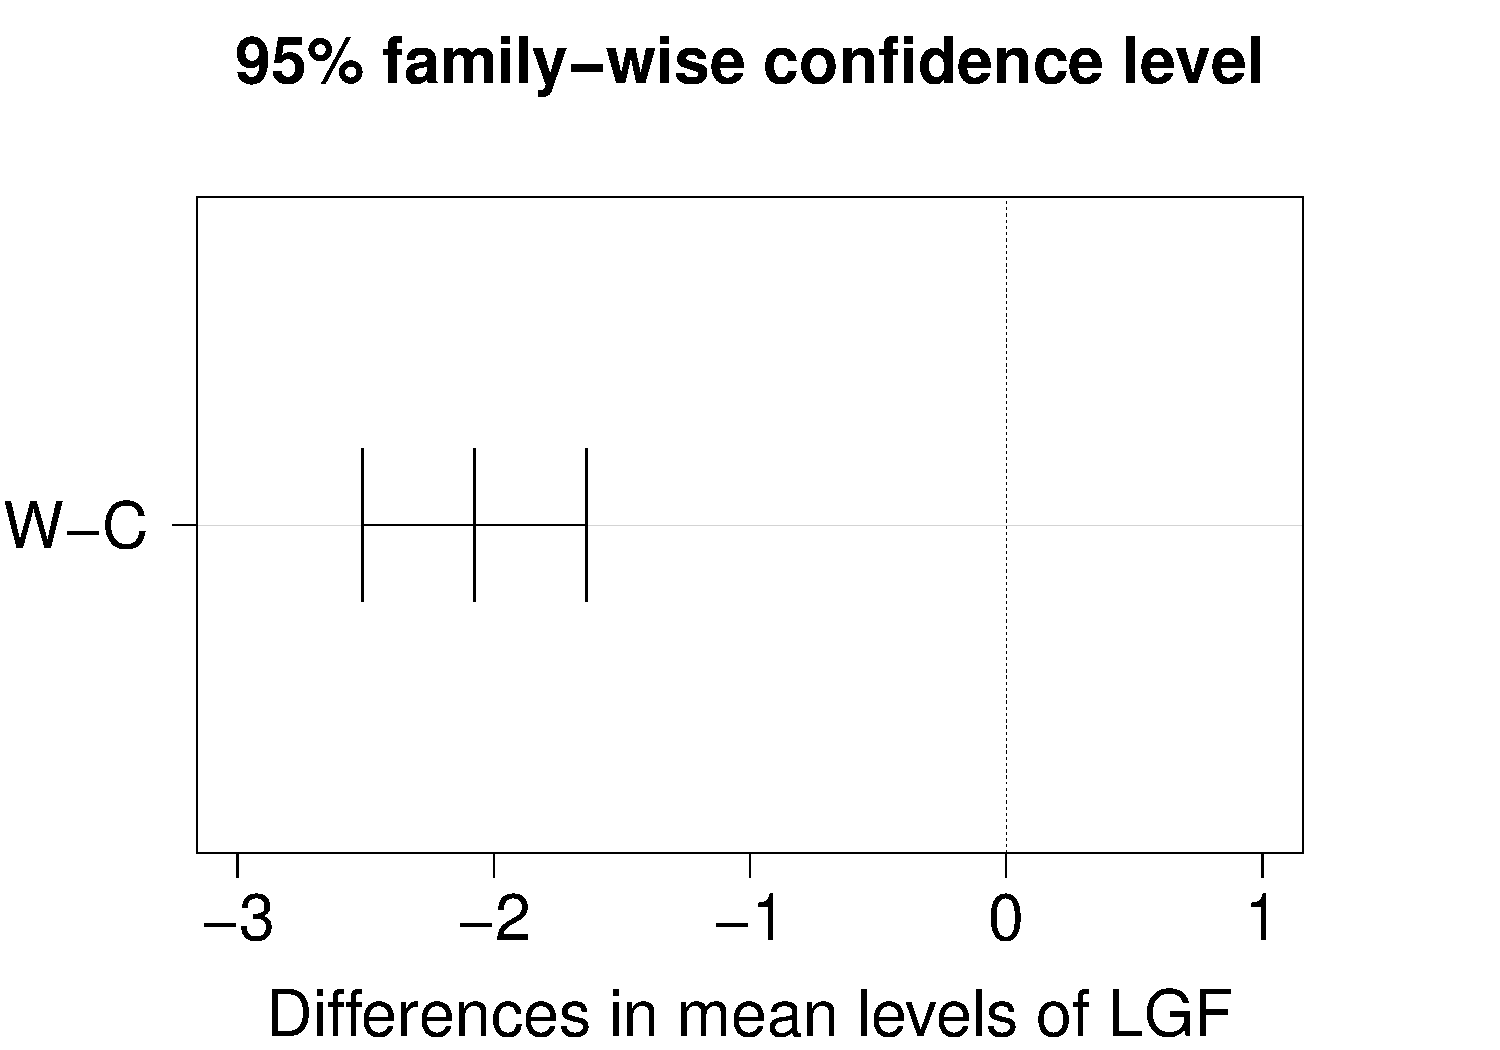
\includegraphics[width=0.21\textwidth]{test_0_auc/LGF}}\hspace{1cm}
\subfloat[M refers to summarization measure and the video of spectra used to generated the low-level descriptors.]{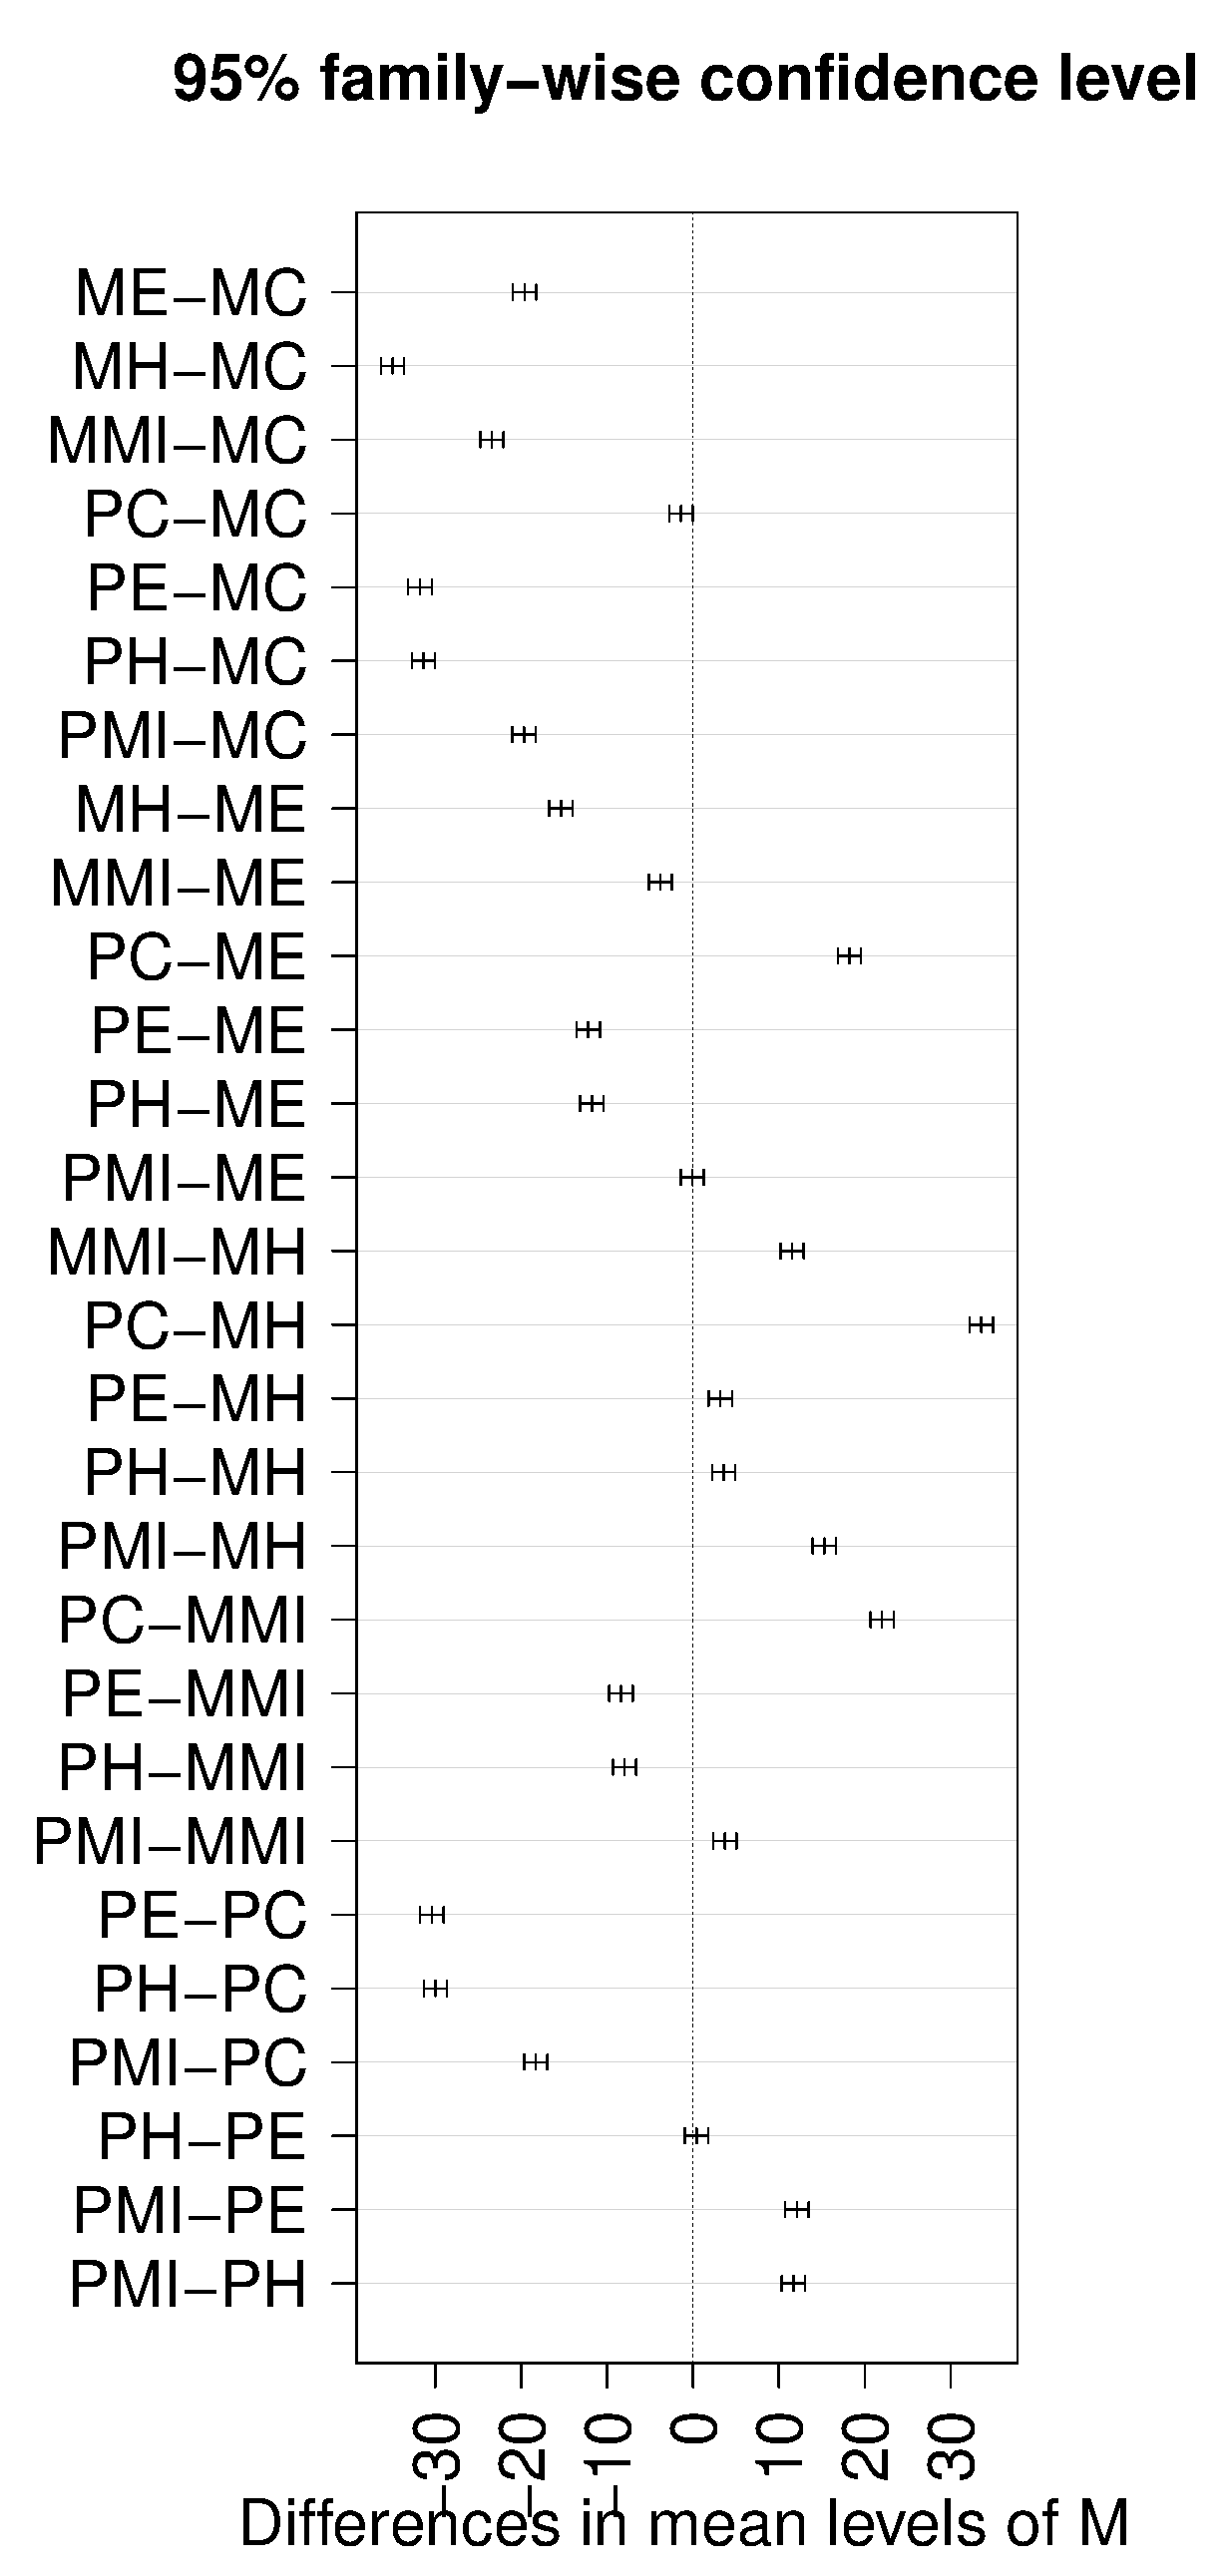
\includegraphics[width=0.35\textwidth]{test_0_auc/M}}\\
\caption{{Confidence interval on the differences between the means of the levels of the factors (a) LGF, and (b) M. For each comparison, the Tukey's HSD test provides an estimation of the differences between mean pairs and their respective confidence intervals, as well the $p$-value for each comparison. All comparisons whose confidence intervals do not contain zero value have a $p$-value lower than $0.05$ and, therefore, are statistically different with a $95\%$ confidence level. (See Table~\ref{table:DOE} to see the description of levels.)\label{fig:llf_pvalues}}}
\end{figure*}

\subsubsection{Mid-Level Descriptor Extraction Parameter Analysis (CS, SDD, DS, and CP)}\label{sec:main_effect_2}
\minor{To construct a discriminative visual codebook, we need to choose the best strategy for selecting the words that compose the visual codebooks (CS) as random or clustering-based,  the visual codebook size (DS), the policy to create the visual codebooks (SDD) as single or class-based, and the pooling and coding strategies (CP).}
%
\begin{figure*}[!ht]
\centering
\subfloat[DS refers to the number of time-spectral visual words present in the visual codebook.]{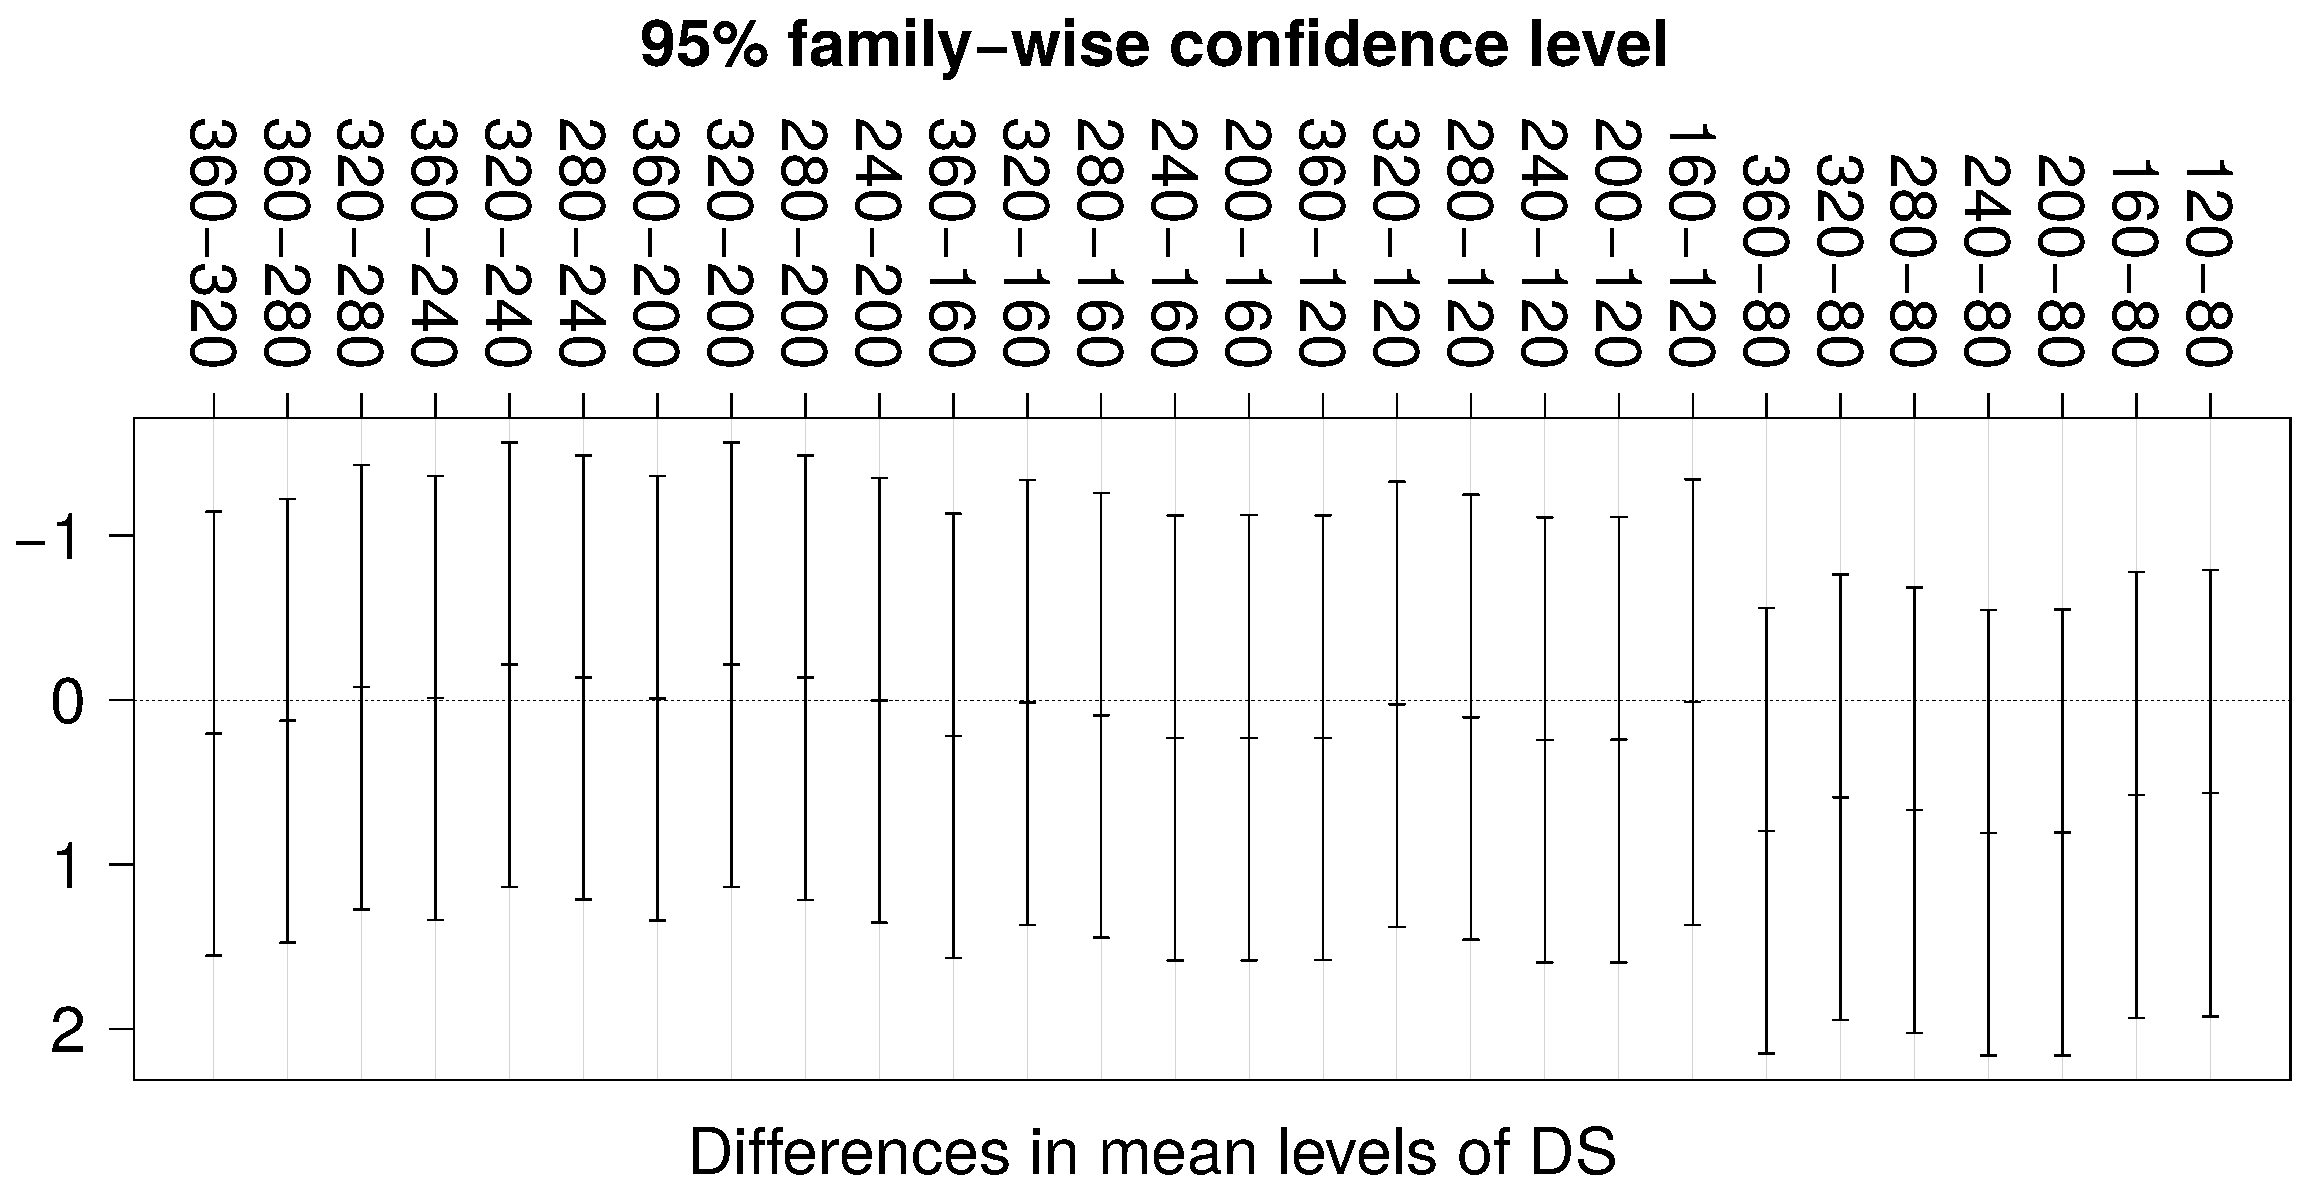
\includegraphics[width=0.3\textwidth]{test_0_auc/DS}} \\
\subfloat[CP denotes the coding and pooling strategies used to build the mid-level descriptors.]{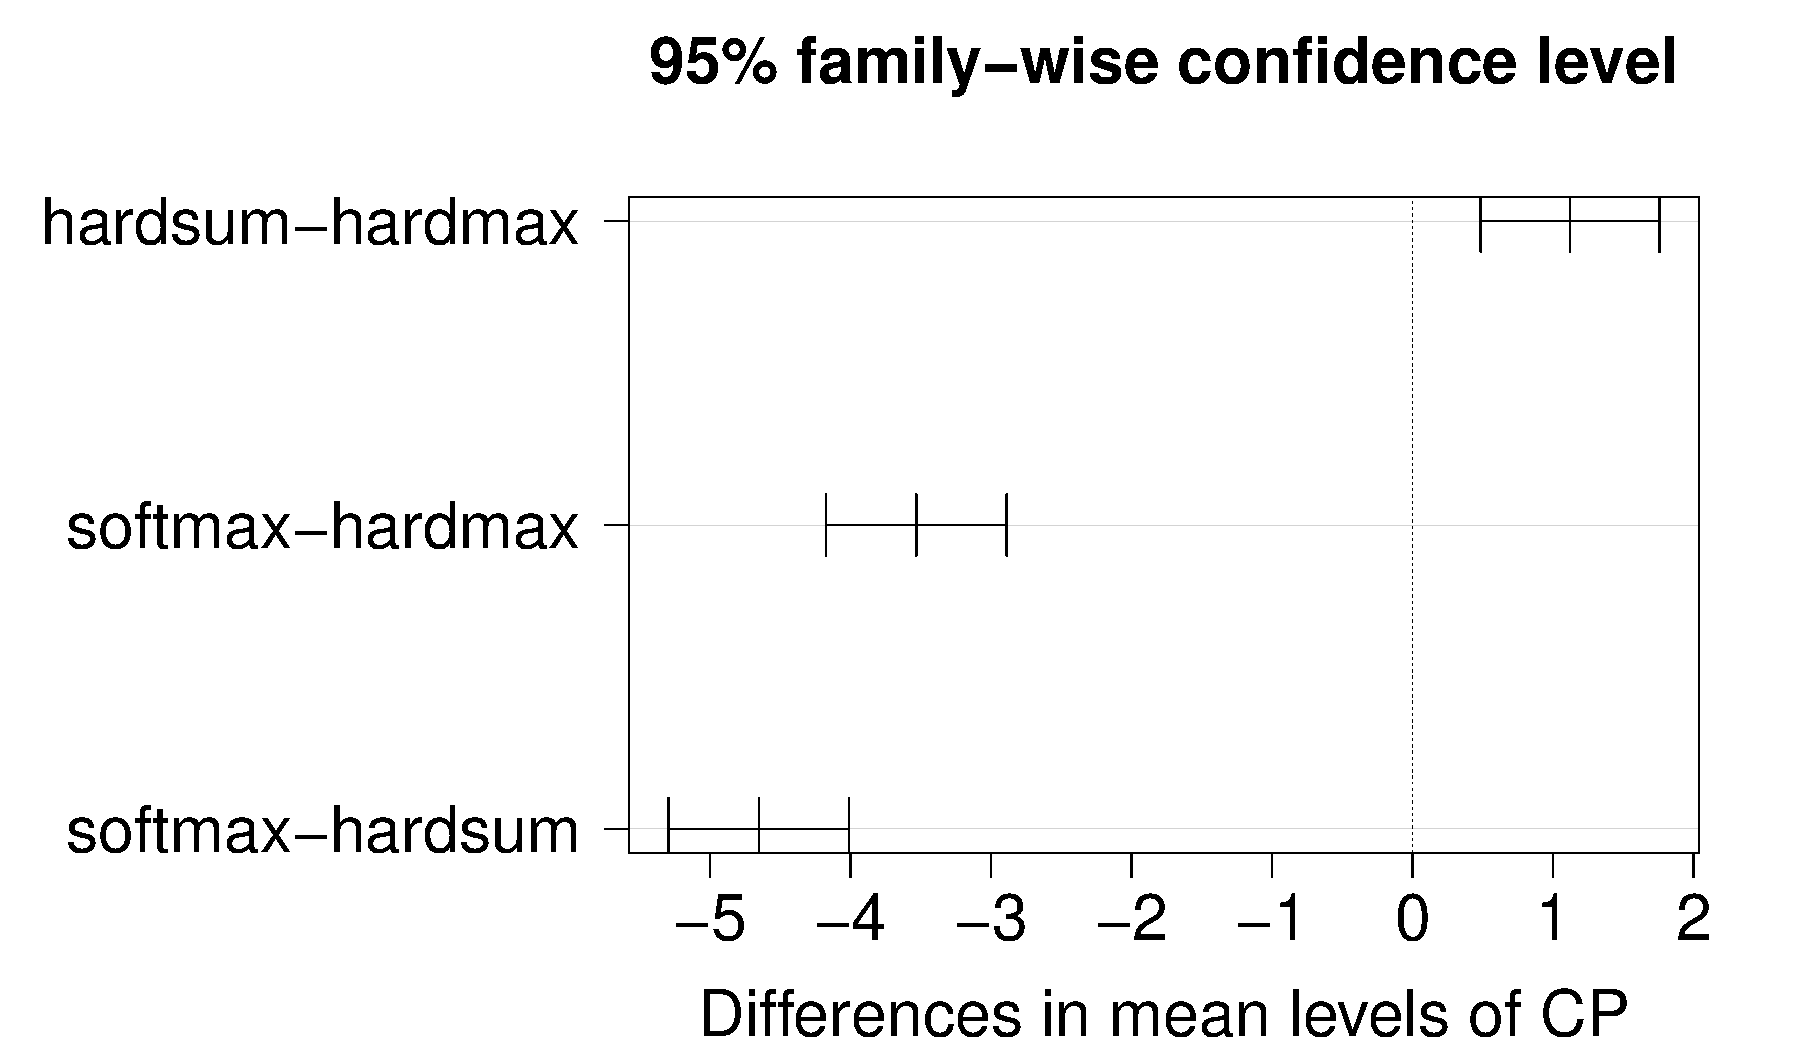
\includegraphics[width=0.25\textwidth]{test_0_auc/CP}}\hspace{5mm}
\subfloat[CS denotes the selection mode of the time-spectral visual words for composing the visual codebook.]{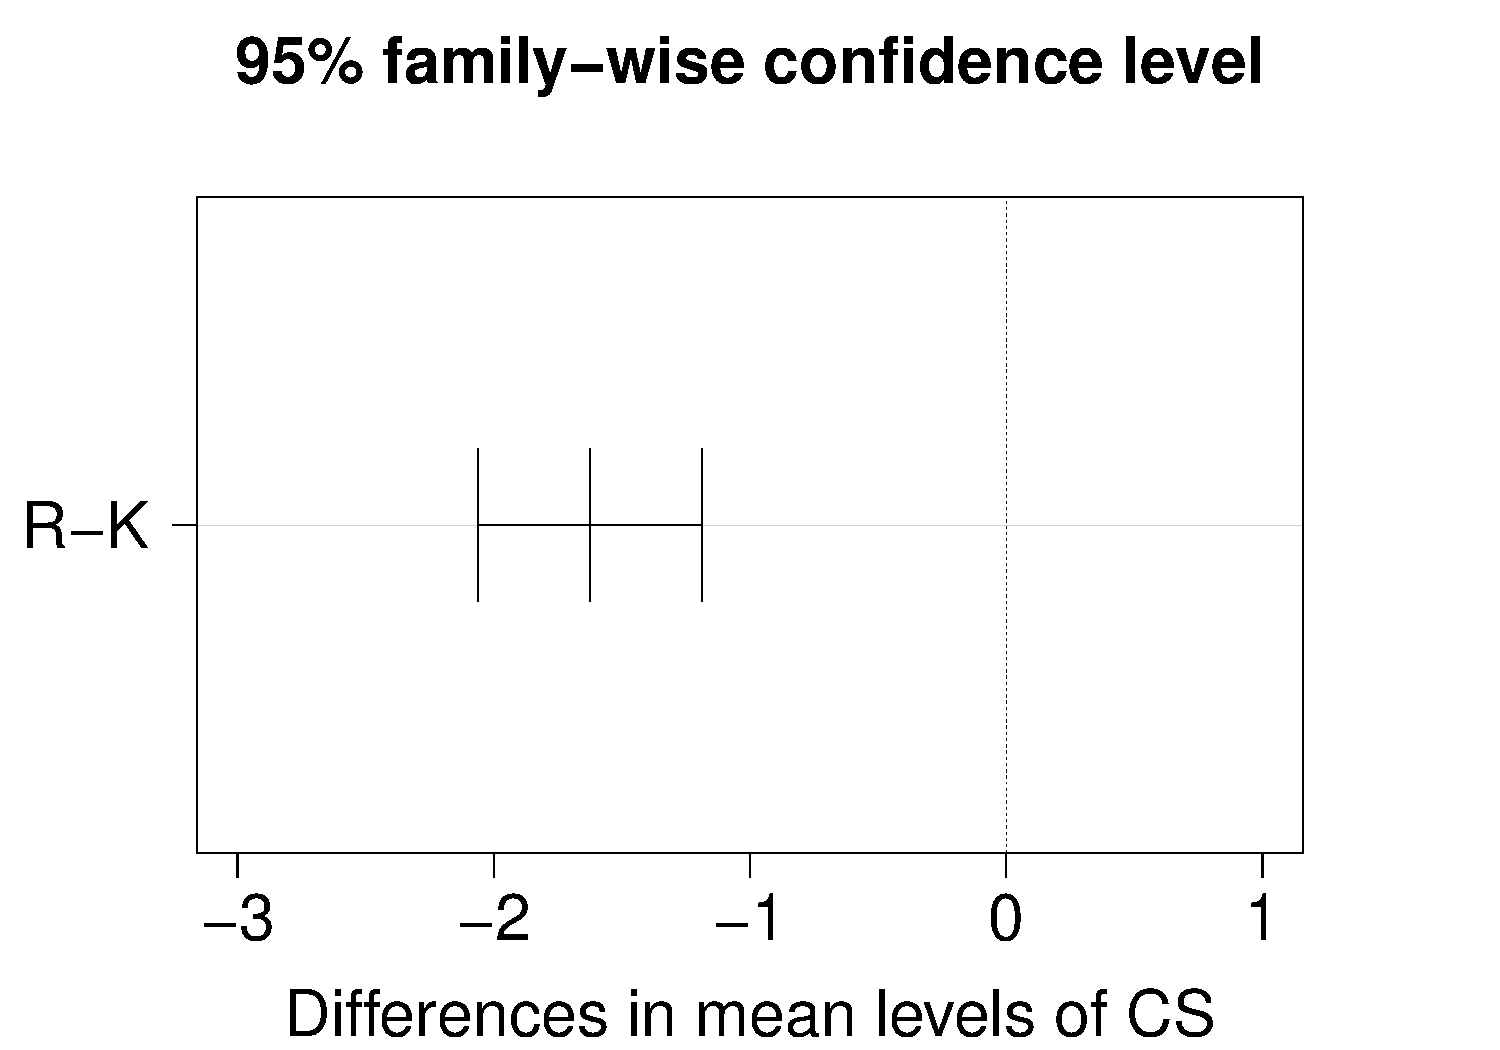
\includegraphics[width=0.22\textwidth]{test_0_auc/CS}}\hspace{2.5mm}
\subfloat[SDD denotes the strategies for generating the visual codebooks, single or class-based visual codebooks.]{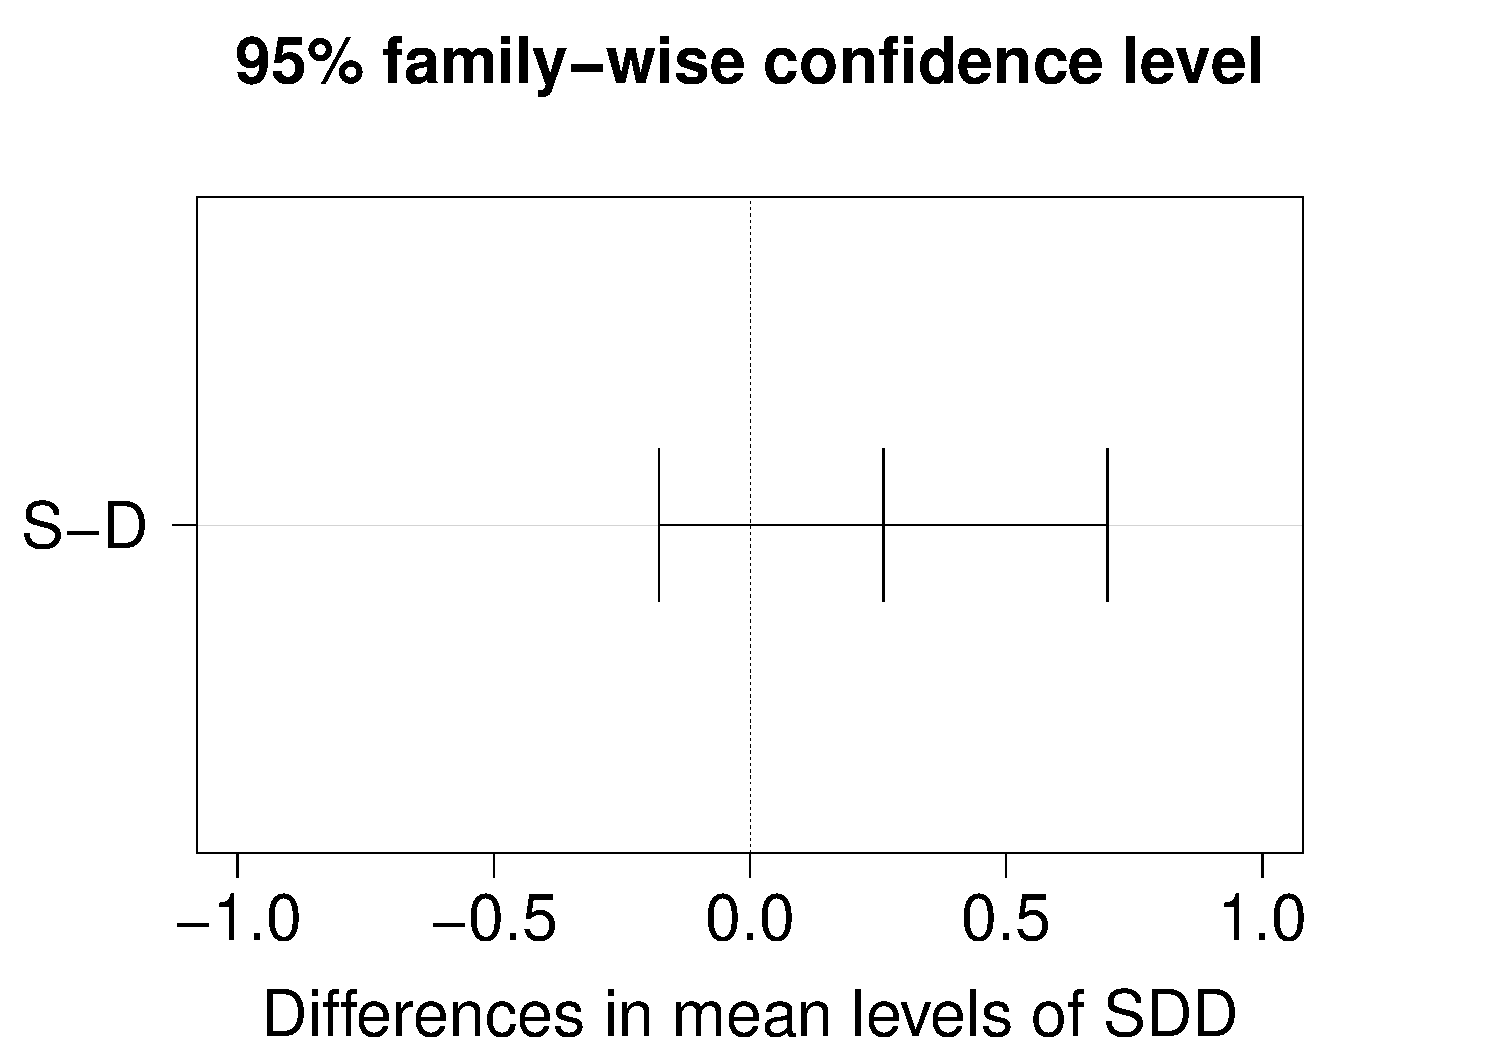
\includegraphics[width=0.2\textwidth]{test_0_auc/SDD}} \\
\caption{Confidence interval of the differences between the means of the levels of the factors (a) DS, (b) CP, (c) CS and (d) SDD. 
All comparisons whose confidence intervals do not contain zero value have a $p$-value lower than $0.05$ and, therefore, are statistically different with a $95\%$ confidence level as it is the case for the comparisons indicated on the (a) $x$ axis and (b-d) $y$ axis. (See Table~\ref{table:DOE} for the description of levels.)}
\label{fig:flf_pvalues}
\end{figure*}

\minor{Fig.~\ref{fig:flf_pvalues} shows the results of the post-hoc test with Tukey's HSD. {In Fig.~\ref{fig:flf_pvalues}(a), we have the results of the statistical analysis for DS parameter (dictionary size), to which was not found statistical significance}. Therefore, we recommend that dictionary size parameter to be optimized according to the application of interest. In turn, Fig.~\ref{fig:flf_pvalues}(b) shows that different pooling and coding processes causes statistically significant impacts on the response variable, and softmax is the recommended choice.}

\minor{In addition, Fig.~\ref{fig:flf_pvalues}(c) shows that the method used to select the words that compose the visual codebook (random vs. clustering-based selection) also presents results that are statistically {significant} with $k$-means being the recommend choice \allan{due to the high performance achieved by models built with visual codebooks generated using $k$-means, during this experiment}. Finally, Fig.~\ref{fig:flf_pvalues}(d) shows that the visual codebook creation strategy (single visual codebook vs. class-based codebooks) does not present statistical difference and, therefore, should also be considered in a future optimization process during the implementation of the method in a real application.}

\subsubsection{Classification Step Parameter Analysis (C)}\label{sec:main_effect_3}
The SVM classifier outperformed PLS classifier with a statistically significant difference  (\textit{$\textit{p}$-value} = $0.00$). We believe that this happened because of the non-linearity of the data as we use a non-linear version of SVM the a linear version of PLS.

\subsubsection{Analysis of Interaction Effects and Choice of the Best Configuration}
\label{sec:best:config}
\minor{After analyzing each factor in isolation, we examine whether there is significant interaction between factors}. In this case, if a small $p$-value is obtained in the interaction effect analysis between two factors, then we can conclude that these factors do not operate independently of each other~\cite{Hayter:CL:2012}. \redmark{Otherwise, there is no evidence of an interaction effect.} 

\minor{First of all, we can see that there is a relationship between the region from which the low-level time-spectral features are extracted (factor LGF) and the spectral information used in the generation of time-spectral descriptors (factor M). When analyzing the magnitude spectrum of the Fourier transform, we see that there is a concentration of low frequency components in the abscissa and ordinate axes. Fig.~\ref{fig:interactions} shows that this interaction between factors LGF and M exists. In addition: (i) we have an increase in the mean of AUC values for measures $MH$, $PH$, $PE$ and $PMI$, when these measures are calculated in the center region of the frames; (ii) we have a decrease in the mean of AUC for measure $PC$; and (iii) we have very small changes in mean values of AUC for $MC$ and $MMI$ when we compare the two strategies for feature extraction.}
%
\begin{figure}[!htb]
\centering
\subfloat[LGF and M interaction. Note that we have a slump in the mean of AUC when setting LGF to W and decrease the number of low-level features.]{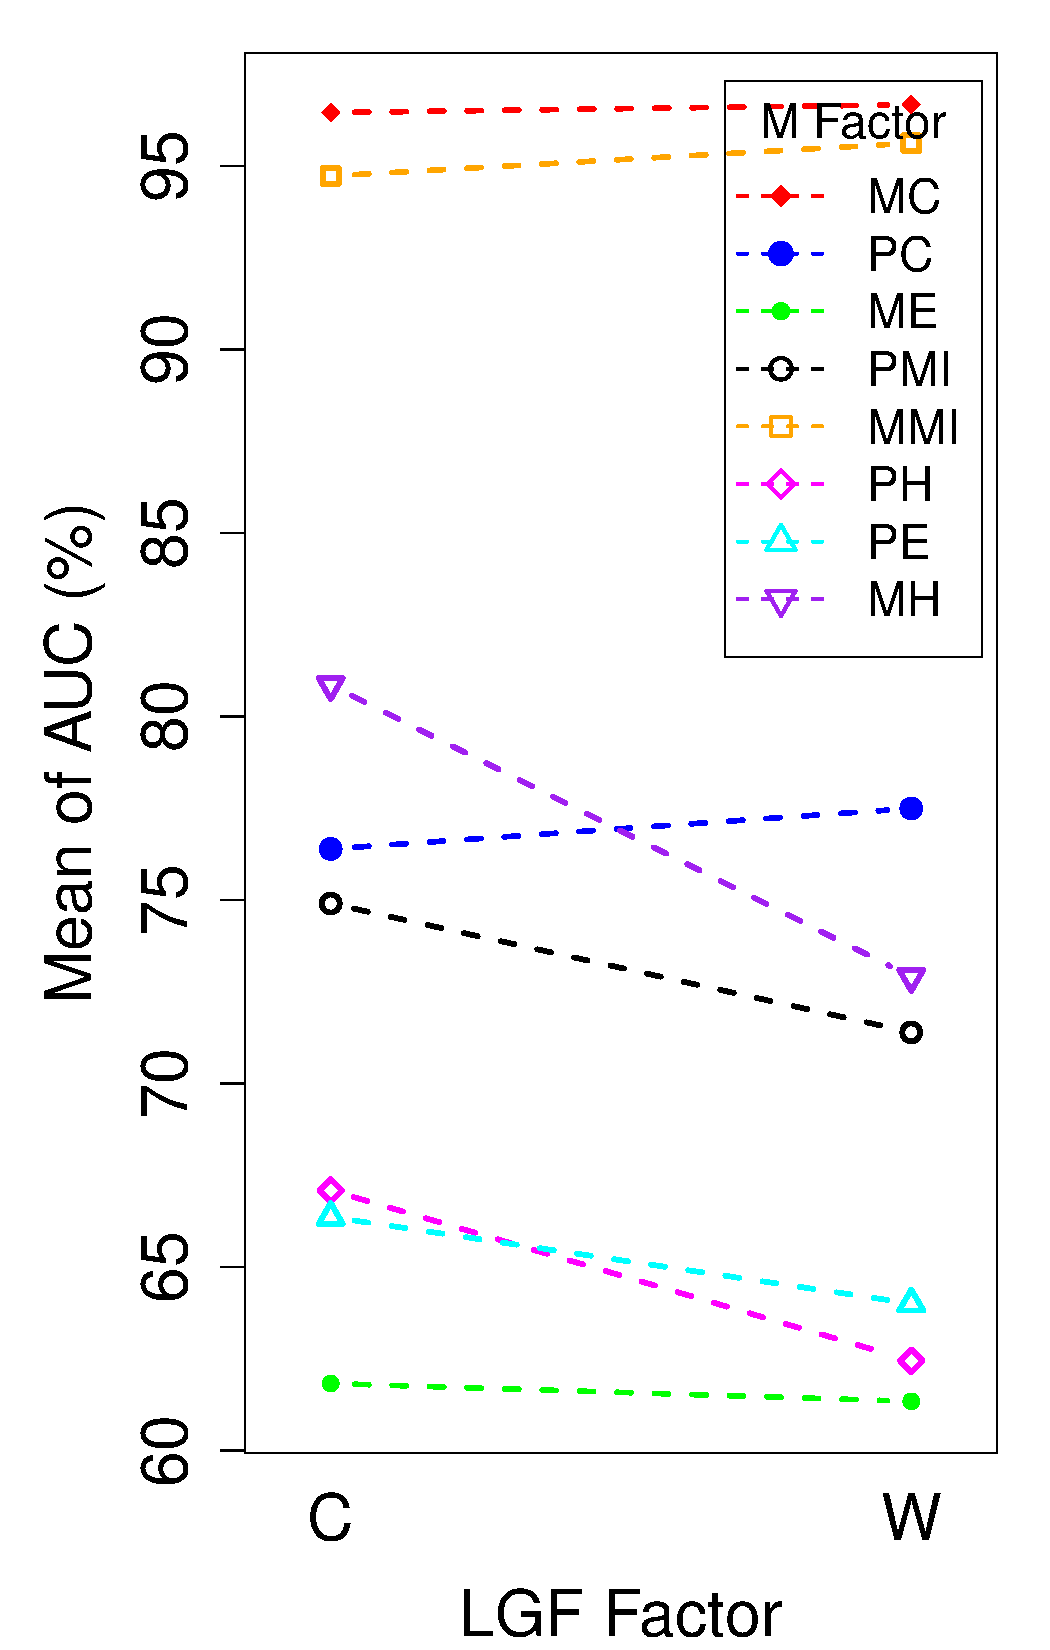
\includegraphics[height=4cm,width=3.5cm]{test_0_auc/LGF_M}}\hspace{0.5mm}
\subfloat[CS and CP interaction. We have a significant increase in the mean of AUC with the hard-assignment when we use $k$-means to select the visual words of the codebooks.]{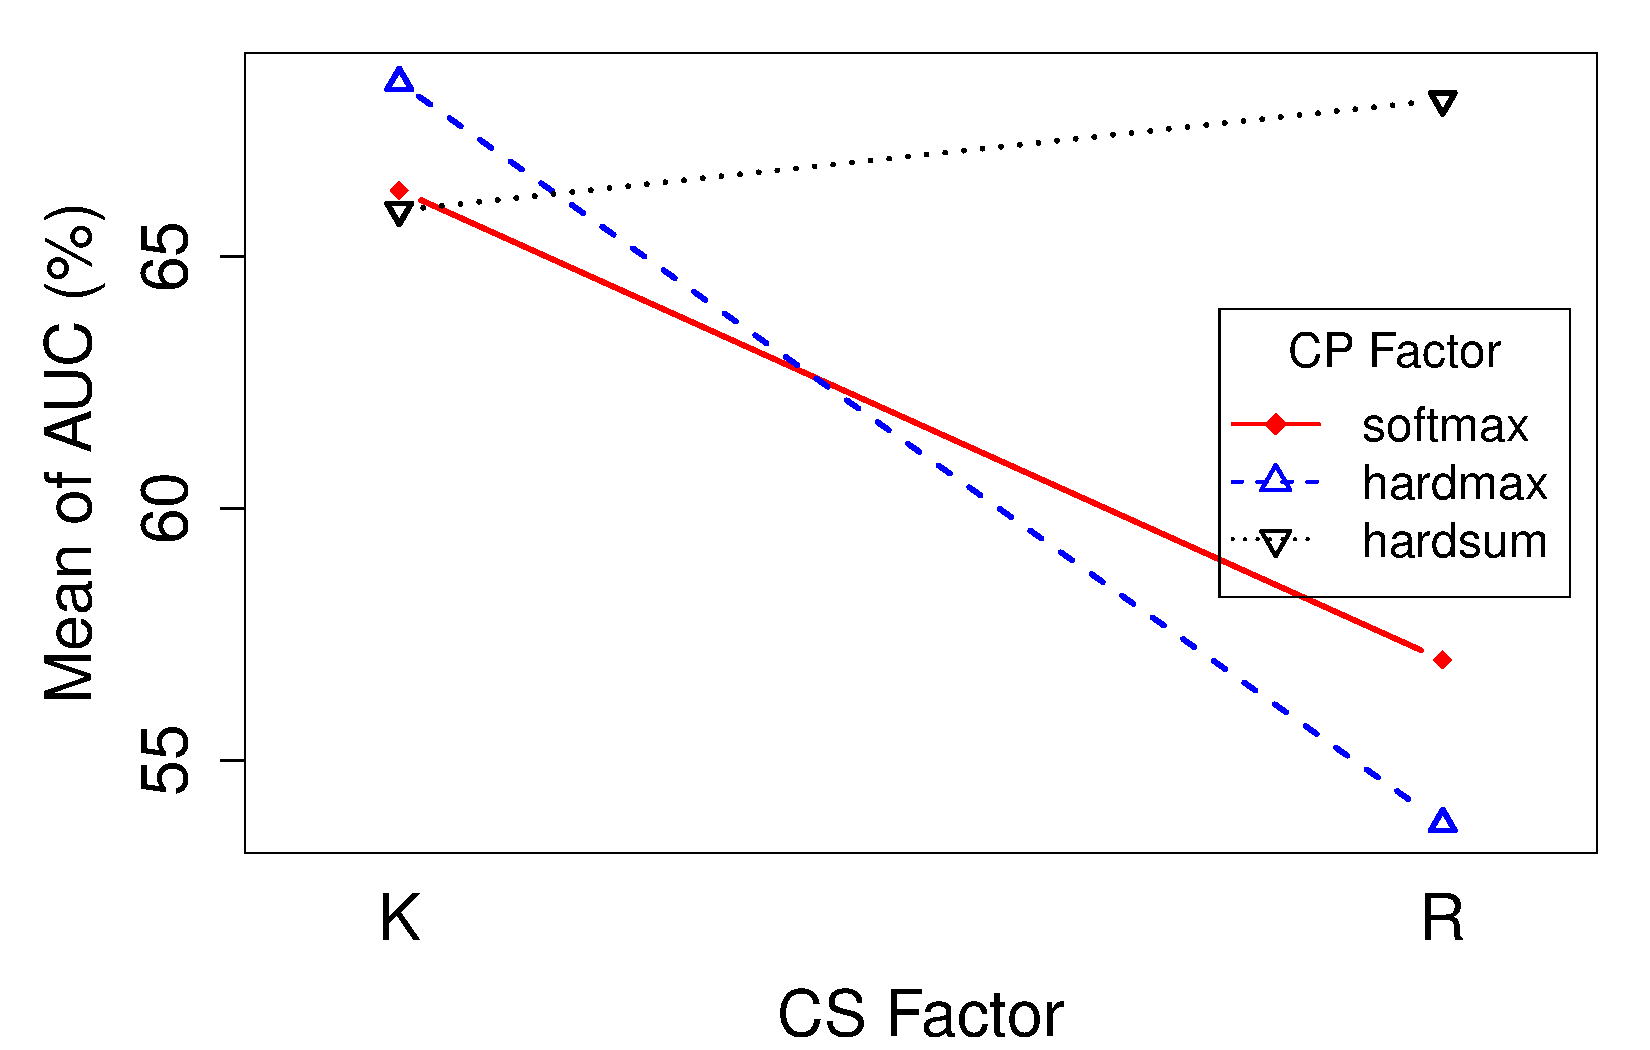
\includegraphics[height=4cm,width=3.5cm]{test_0_auc/CS_CP}}\hspace{0.05mm}
\caption{{Interaction plots between pairs of factors (a) LGF$\times$M and (b) CS$\times$CP. The factor LGF denotes the region in the frame considered for extracting the low-level features, while factor M denotes the statistical measures considered for describing the information of the temporal cubes. Finally, the factor CS denotes the mode of selection of the visual words {from visual codebooks} and the factor CP refers to the strategies used in the coding and pooling process. (See Table~\ref{table:DOE} to see the description of levels.)}}
\label{fig:interactions}
\end{figure}

Finally, the form of selecting the visual words (factor CS) and the method of coding and pooling used in the construction of the dictionaries (factor CP) also presents an interesting interaction. Both factors significantly influence the results, but not in isolation. Fig.~\ref{fig:interactions}(b) shows that the results obtained with hardmax, hardsum and softmax are worse when the visual words are chosen randomly instead of through clustering. 

\subsection{Summary After Analyzing Different Factors and Levels}
{The proposed method presents better results using time-spectral features extracted from magnitude spectrum videos considering the whole frames of a video and using the correlation measure from time-spectral features for generating the time-spectral descriptors.}

{The class-based codebooks \minor{outperform} the single codebook and the selection strategy of the visual words that best fits to the spoofing detection problem is the $k$-means clustering. The most appropriate size for codebooks is $320$ visual words and the softmax outperformed the other coding and pooling strategies. With this configuration, we obtained an AUC of $99.46\%$ and an HTER of $2.75\%$, considering the \allan{test set} of the Replay-Attack dataset~\cite{Chingovska:BIOSEG:2012}. Next, we show experiments and results for this method using this final configuration.}

\subsection{Results}\label{subsec:soa_comparison}
\minor{This section compares the proposed method with others in the literature for the {Replay-Attack~\cite{Chingovska:BIOSEG:2012}, CASIA~\cite{Zhang:ICB:2012} and 3DMAD~\cite{Erdogmus:BIOSIG:2013} datasets. In all experiments, we used the best configuration of the proposed method as discussed in the last section. The parameters that did not present statistical significance (DS and SDD), were fine-tuned for each dataset.}}

\subsubsection{Replay-Attack Dataset}\label{subsec:ra_results}

\minor{We first consider the validation Protocol I~(c.f., Sec.~\ref{subsec:Protocol}) and the Replay-Attack dataset. Table~\ref{table:our_reults} shows the results for the three types of attacks available in this set. Fig.~\ref{fig:det_plot_replay_attack}(a) shows  that attacks performed with high-quality samples are more difficult to detect (HTER of $5.94\%$). This result was expected as high-quality fake samples usually contain less artifacts revealing an attack}.

\minor{In turn, video-based and photo-based attacks were easily detected (HTER of $0.63\%$). Note that video-based spoofing attacks are more susceptible to blurring effects, whereas the photo-based attacks show a large amount of flickering effects due to printing defects. Fig.~\ref{fig:det_plot_replay_attack}(b) shows results obtained considering fixed-support and hand-based attacks, separately. We believe that hand-based attacks are easier to be detected given that small movements of the impostor user during the attack generate more artifacts in the biometric sample causing more disturbances in the \redmark{frequency components.}}
%
\begin{table}[!htb]
\centering
%\linethickness{1.5mm}
\caption{Performance results for the Replay-Attack Dataset.}
\label{table:our_reults}
\begin{tabular}{lcccc}
\topline
\headcol \multicolumn{1}{c}{Dataset} & FAR	& FRR 	& HTER 	& AUC	\\
\midline
High-definition attack 	  & $10.63$ & $1.25$ & $5.94$ & $98.77$ \\
\rowcol Mobile attack 	  & $0.00$  & $1.25$ & $0.63$ & $99.95$  \\
Print attack 			  & $0.00$  & $1.25$ & $0.63$ & $99.86$ \\

\rowcol Hand-based attack & $1.00$  & $1.25$ & $1.13$ & $99.87$  \\
Fixed-support attack 	  & $7.50$  & $1.25$ & $4.38$ & $99.03$ \\

\rowcol \textbf{Overall test set} 
& $\mathbf{4.25}$ &  $\mathbf{1.25}$ &  $\mathbf{2.75}$ & $\mathbf{99.46}$ \\
\bottomlinec
\end{tabular}
\end{table}
%
\begin{figure}
\centering
\subfloat[]{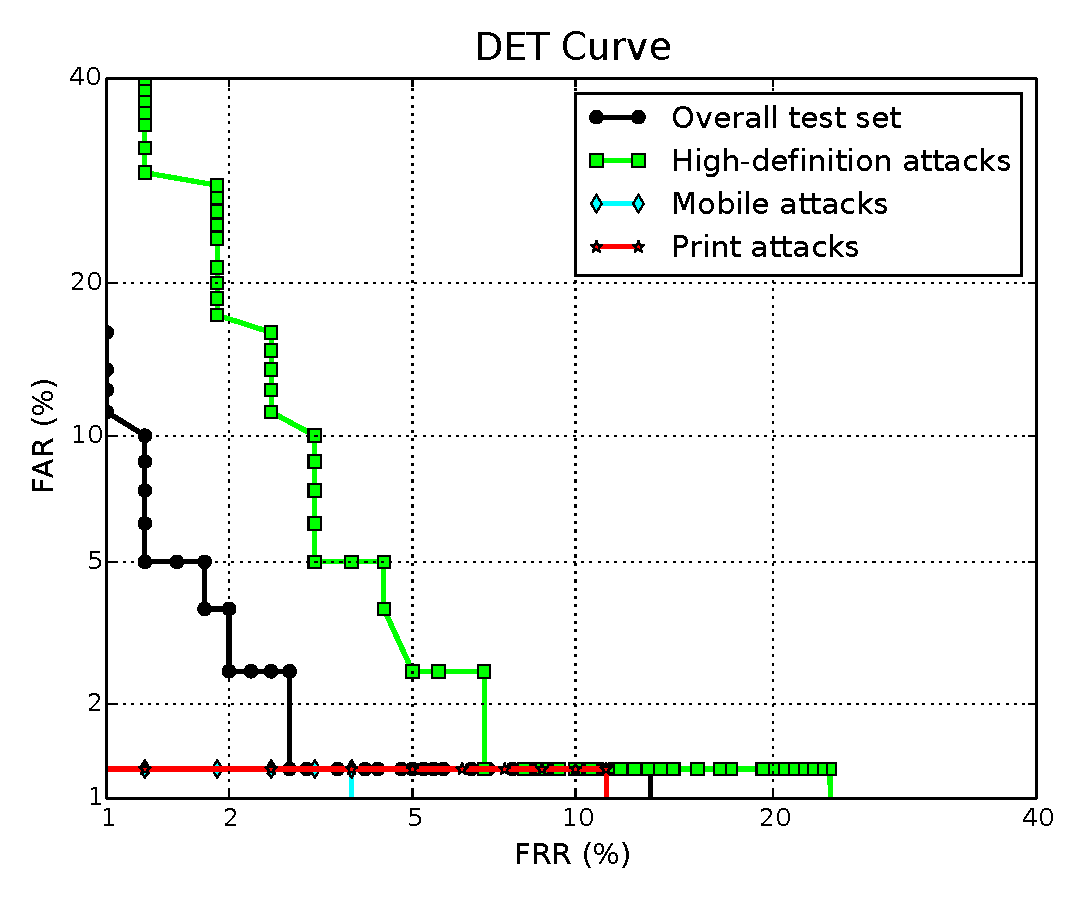
\includegraphics[width=0.45\linewidth]{det_plot_replay_attacks.pdf}}
\subfloat[]{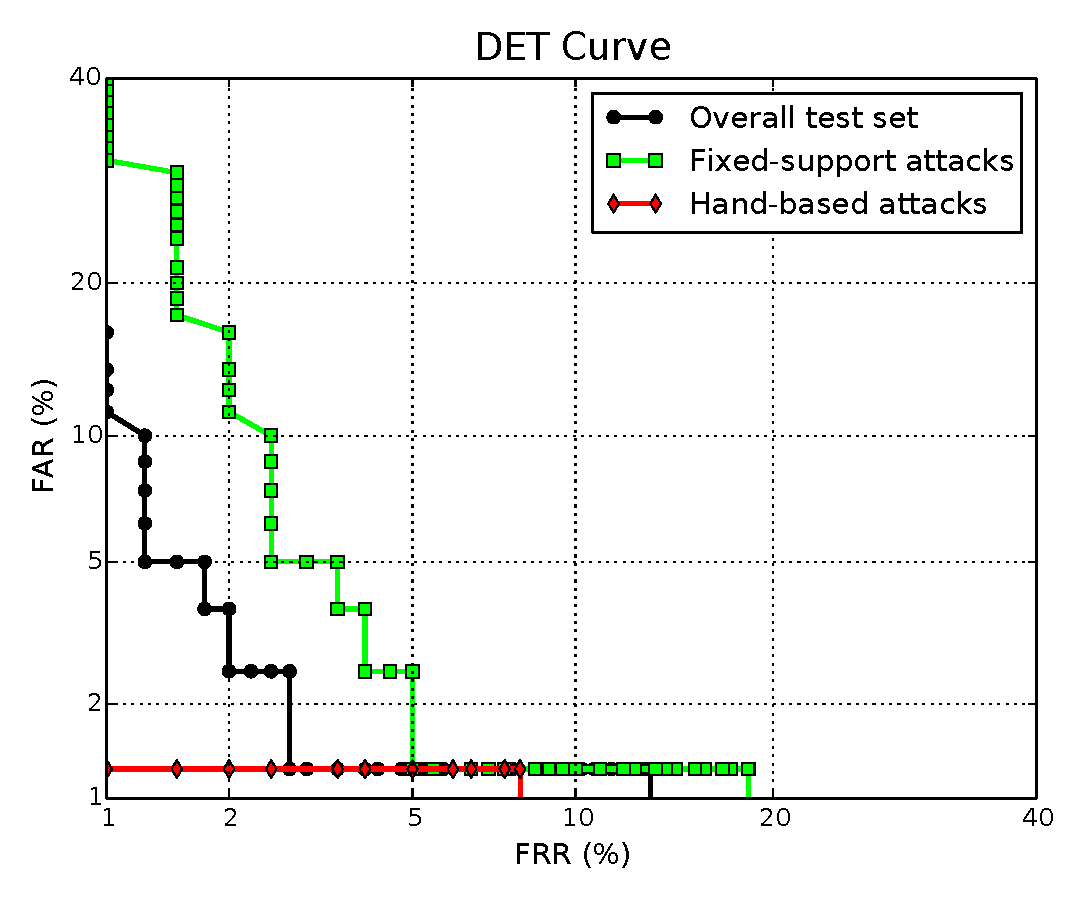
\includegraphics[width=0.45\linewidth]{det_plot_replay_hand_fixed.pdf}}
\caption{{Results obtained on Replay-Attack dataset for each type of attack using fixed-support (a) in contrast with hand-based attacks (b).}}
\label{fig:det_plot_replay_attack}
\end{figure}


\subsubsection{CASIA Face Anti-Spoofing Dataset}\label{subsec:casia_results}
In this experiment, we evaluate the proposed method using the Protocol II (c.f., Sec.~\ref{subsec:Protocol}) and CASIA dataset. 

Table~\ref{table:our_reults_casia} shows the results obtained for the seven {scenarios} of attacks available in this dataset. Fig.~\ref{fig:det_plot_casia}(a) shows that video-based and warp-photo spoofing attacks are easier to be detected by the proposed method (HTER of $ \approx 8\%$). On the other hand, the cut-based spoofing attacks are more difficult to be detected (HTER of $22.22\%$). \redmark{One possible reason for cut-based attacks to be more difficult for detecting is that during an attempted attack based on cut-photos, the photographs are practically in the same position during all the time, generating fewer artifacts along time, whereas for the attempted attacks based on warped-photos, the photographs are bent during the attack to simulate facial motion. In addition, we believe that video-based attacks were easier to be detected because of the inevitable downsize of the high-resolution samples by the screen device used during attack, as also reported by CASIA's authors~\cite{Zhang:ICB:2012}. In this case, many evidences of attempted attacks are generated and added to the fake sample.} 

As for the quality of the acquisition (Fig.~\ref{fig:det_plot_casia}(b)), the proposed method showed better results for attacks carried out with low-quality videos. An interesting result is the best performance of the method to deal with high-resolution videos than normal quality videos. \redmark{We believe that any conclusion would be precipitous because many factors can influence the noise level of a sensor such as sensor imperfections (e.g., appearance of hot pixels, dead pixels, as well as pixel traps under different acquisition conditions). Several works in the literature have explored these issues. For instance, thermal action has a considerable impact over pattern noise of a digital camera and appearance of defective pixels~\cite{Chen2007,Lukas:TIFS:2006,Rocha:2011:VUC}. As we do not assure that the captures/recaptures happened under similar acquisition conditions, it is wiser only to point out the existence of classification differences in this case.}
%
\begin{table}[!htb]
\centering
%\linethickness{1.5mm}
\caption{Performance results for the CASIA dataset.}
\label{table:our_reults_casia}
\begin{tabular}{lcccc}
\topline
\headcol \multicolumn{1}{c}{Dataset} & FAR	& FRR 	& HTER 	& AUC	\\
\midline
		Low quality		  & $10.00$ & $10.00$ & $10.00$ & $98.11$ \\
\rowcol Normal quality    & $17.78$ & $20.00$ & $18.89$ & $87.67$ \\
		High quality 	  & $13.33$ & $13.33$ & $13.33$ & $95.04$ \\
\rowcol Warp photo attack & $7.78$  &  $8.89$ &  $8.33$ & $96.05$ \\
		Cut photo attack  & $22.22$ & $22.22$ & $22.22$ & $87.27$ \\
\rowcol Video attack 	  &  $8.89$ &  $8.89$ &  $8.89$ & $96.41$ \\
\textbf{Overall Attack}   & $\mathbf{14.07}$ &  $\mathbf{14.44}$ &  $\mathbf{14.26}$ & $\mathbf{93.25}$ \\
\bottomline
\end{tabular}
\end{table}
%
\begin{figure}
\centering
\subfloat[]{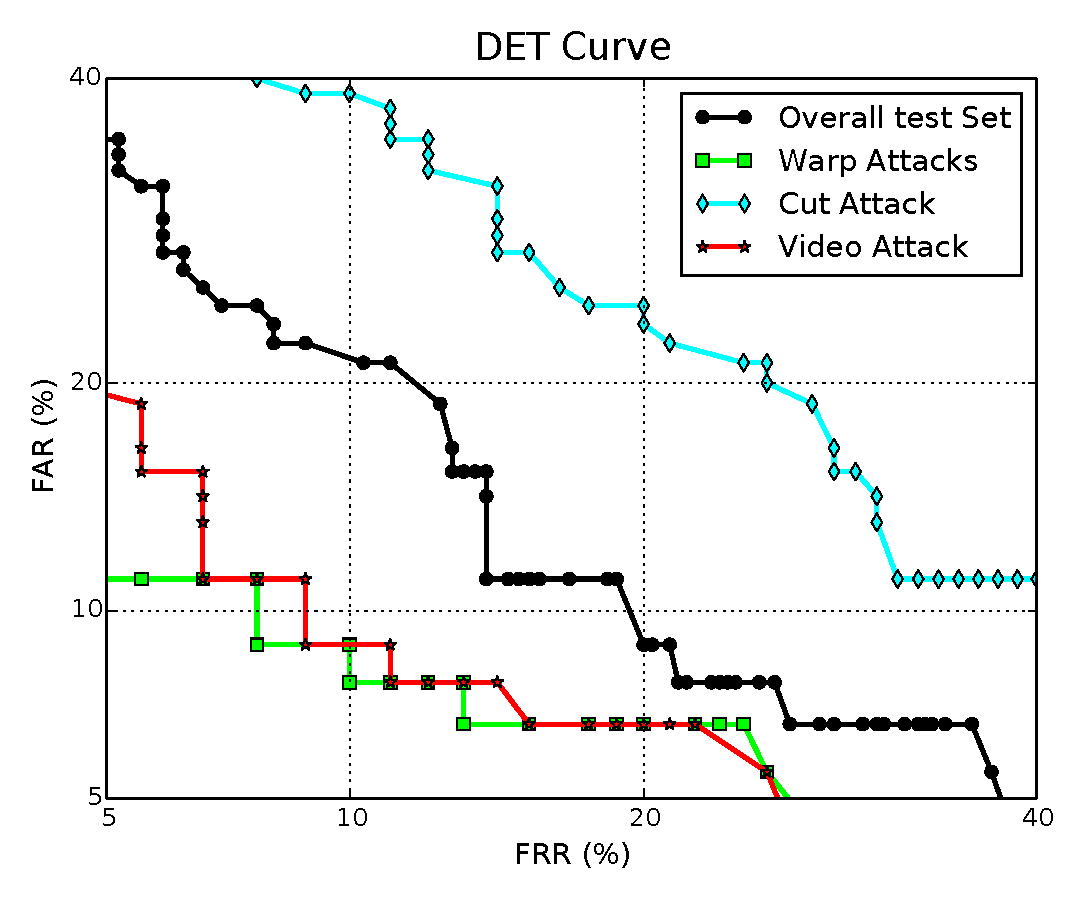
\includegraphics[width=0.45\linewidth]{det_plot_casia_type_attacks.pdf}}
\subfloat[]{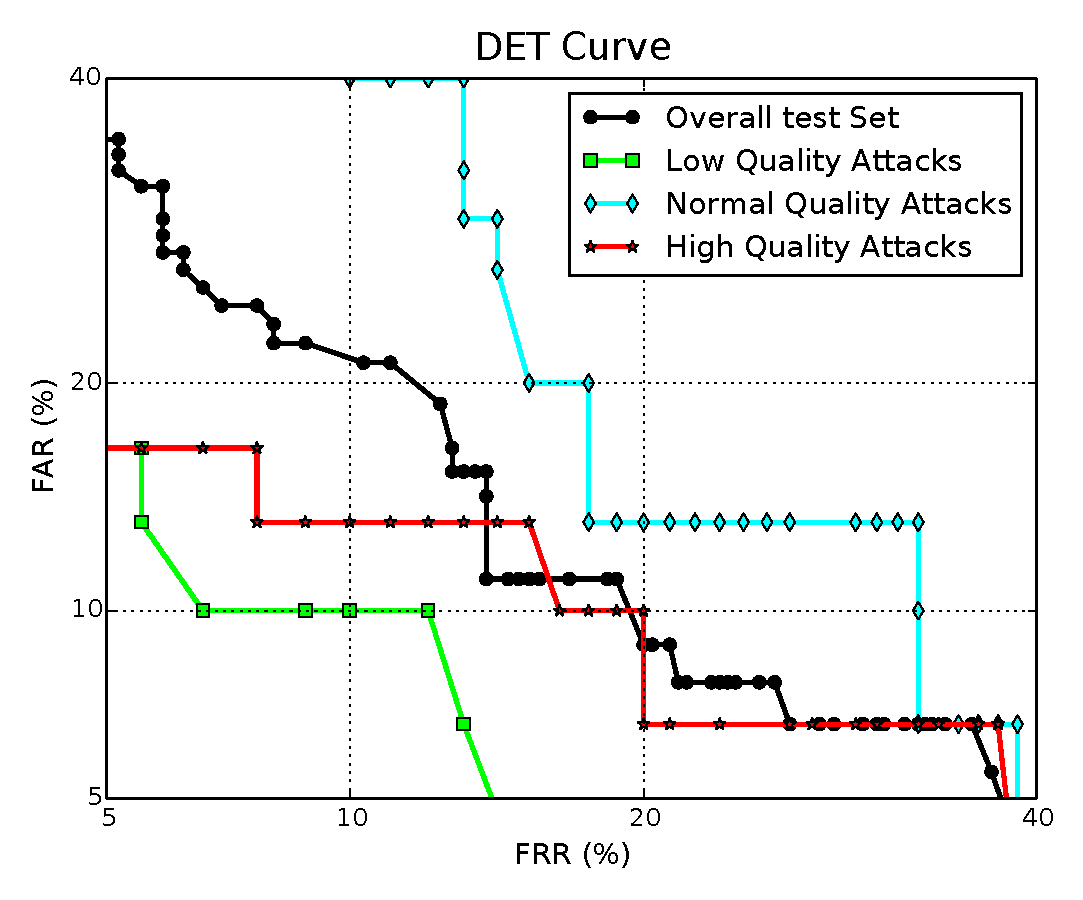
\includegraphics[width=0.45\linewidth]{det_plot_casia_qualy.pdf}}
\caption{Results obtained on CASIA dataset for the three type of attacks (a) and for the three quality of attack (b).}
\label{fig:det_plot_casia}
\end{figure}


\subsubsection{3DMAD Dataset}\label{subsec:3dmad_results}
We now turn our attention \minor{to evaluate} the proposed method for mask-based spoofing attack detection {using the Protocol IV (c.f., Sec.~\ref{subsec:Protocol})}. Using the official \minor{dataset protocol}, the proposed method obtained an AUC of $96.16\%$ and an HTER of $8.0\%$.

\minor{Erdogmus et al.~\cite{Erdogmus:BTAS:2013} reported an HTER of $0.95\%$ using block-based LBP features (local features) and the Linear Discriminant Analysis (LDA) classifier. This performance difference is somewhat explained due to the different validation protocol used. Erdogmus et al. used an $1000$-fold cross validation method and, in each fold, the clients from the dataset were randomly assigned into training, development and test sets. In our case, we randomly divided the clients from dataset and assigned them into training, development and test set only once. Even so, the proposed method outperforms other techniques using global LBP, whose HTERs reported by Erdogmus et al. were all above $10.0\%$.}


\subsubsection{UVAD Dataset}\label{subsec:uvad_results}
In this experiment, we evaluate the proposed method using the Protocol III (c.f., Sec.~\ref{subsec:Protocol}) and UVAD dataset. We also evaluate the proposed method considering LBP-based and motion-based countermeasure methods. 

According to Pereira et al.~\cite{Pereira:ICB:2013}, the correlation method presents an HTER of $11.79\%$ on Replay-Attack. {In turn,} LBP$_{8,1}^{u2}$~\cite{Chingovska:BIOSEG:2012} was effective to characterize the artifacts embedded in the attack videos on Replay-Attack obtaining an HTER of $15.16\%$. In the UVAD dataset, however, both methods obtained a more modest performance as Table~\ref{tab:antispoofing_uvad} shows. With respect to LBP$_{8,1}^{u2}$ method, for instance, the proposed method reduces the classification error in about $36\%$.
%
\begin{table}[!ht]
	\centering
	\caption{Comparison among LBP-based approach~\cite{Chingovska:BIOSEG:2012}, motion-based approach~\cite{Anjos:IJCB:2011} and the proposed method on the UVAD dataset.}
	\label{tab:antispoofing_uvad}
	\begin{tabular}{cccc}
		\topline
		\headcol \textbf{Methods}                         & \textbf{FAR (\%)} & \textbf{FRR (\%)} & \textbf{HTER (\%)} \\ 
		\midline
		Correlation~\cite{Anjos:IJCB:2011}				  & $81.60$ & $14.56$ & $48.06$ \\
		\rowcol LBP$_{8,1}^{u2}$~\cite{Chingovska:BIOSEG:2012}    & $27.41$ & $66.04$ & $46.72$ \\
		\textbf{Proposed Method} & $\mathbf{44.73}$ & $\mathbf{15.00}$ & $\mathbf{29.87}$ \\
		\bottomline		
	\end{tabular}
\end{table}


%Note that our method was trained with the Replay-Attack dataset and tested with 3DMAD dataset, while the method proposed by Erdogmus~\cite{Erdogmus:BTAS:2013} was trained and tested with samples of the same dataset. Even in with the differences existing between the Replay-Attack and 3DMAD dataset (e.g., acquisition sensor, type of attack performed) in this cross-dataset validation protocol, achieved optimal results, which is a remarkable achievement for spoofing detection research.
%%
%\begin{table}[!htb]
%\centering
%%\linethickness{1.5mm}
%\caption{Results (HTER) obtained with our method and with the one proposed method by Erdogmus et al.~\cite{Erdogmus:BTAS:2013} using the 3DMAD dataset.}
%\label{table:3dmad_result}
%\begin{tabular}{lr}
%\toprule
%\multicolumn{1}{c}{Methods} & HTER (\%) \\
%\toprule
% Erdogmus et al.~\cite{Erdogmus:BTAS:2013} & $0.95$ \\
% Proposed Method &  $8.00$ \\
%\bottomrule
%\end{tabular}
%\end{table}

\subsubsection{Comparison with State-of-the-Art Methods for CASIA and Replay-Attack Datasets}

In this section, we compare the proposed method with others \minor{available} in the literature for Replay-Attack and CASIA datasets. Table~\ref{table:CSA} shows results for the Replay-Attack Dataset. The proposed method outperforms the ones based on texture analysis~\cite{Chingovska:BIOSEG:2012,Maatta:IJCB:2011,Pereira:JIVP:2014} and also methods based on motion analysis~\cite{Anjos:IJCB:2011}. It was also more effective than methods based on fusion schemes reported by Pereira et al.~\cite{Pereira:ICB:2013} and Komulainen et al.~\cite{Komulainen:ICB:2013}, with a relative error reduction (RER) of \allan{$67.69\%$ and $46.18\%$}, respectively.
%
\begin{table}[!htb]
\centering
%\linethickness{1.5mm}
\caption{Comparison among the existing methods. The first column shows the HTERs reported by the authors, whereas the second column shows the Relative Error Reduction (RER) obtained with the proposed method. The reported HTERs were obtained using the original Replay-Attack Dataset~\cite{Chingovska:BIOSEG:2012} protocol. \allan{The results highlighted with~$\dagger$~and~$\ddagger$~were reported by Chingovska et al.~\cite{Chingovska:BIOSEG:2012} and Pereira et al.~\cite{Pereira:ICB:2013}, respectively.}}
\label{table:CSA}
\begin{tabular}{lcc}
\topline
\headcol \multicolumn{1}{c}{Methods} & HTER (\%) & RER (\%) \\
\midline
 Chingovska et al.~\cite{Chingovska:BIOSEG:2012} & {15.16} & \allan{81.86} \\
 \rowcol Pinto et al.~\cite{Pinto:TIFS:2015} & 14.27 & \allan{80.73} \\
 \allan{M\"{a}\"{a}tt\"{a} et al.}~\cite{Maatta:IJCB:2011} & 13.87$^\dagger$ & \allan{80.17} \\
 \rowcol \allan{Anjos and Marcel}~\cite{Anjos:IJCB:2011} & 11.79$^{\ddagger}$ & \allan{76.68} \\
 Pereira et al.~\cite{Pereira:ICB:2013} & 8.51 & \allan{67.69} \\
 \rowcol Pereira et al.~\cite{Pereira:JIVP:2014} & 7.60 & \allan{63.82} \\
 Komulainen et al.~\cite{Komulainen:ICB:2013} & 5.11 & \allan{46.18} \\
 \rowcol \textbf{Proposed Method} &  \textbf{2.75} & 0 \\
\bottomlinec
\end{tabular}
\end{table}

Table~\ref{table:soa_casia} shows a comparison among the proposed method and others reported in the literature for CASIA dataset. The proposed method is on par with the best ones in the literature.
%
\begin{table}[!htb]
\centering
%\linethickness{1.5mm}
\caption{Comparison among the proposed method and others available in the literature. According to the authors of the proposed methods, EERs reported were obtained using the original CASIA Dataset~\cite{Zhang:ICB:2012} protocol.}
\label{table:soa_casia}
\begin{tabular}{lr}
\topline
\headcol \multicolumn{1}{c}{Methods} & EER (\%) \\
\midline
 DoG Baseline.~\cite{Zhang:ICB:2012} & 17.0 \\
 \rowcol LBP$_{8,1}^{u2}$.~\cite{Pereira:JIVP:2014} & 16.0 \\
 LBP-TOP$_{8,8,8,1,1,1}^{u2}$.~\cite{Pereira:JIVP:2014} & 10.0 \\
 \rowcol \textbf{Proposed Method}  &  \textbf{14.0} \\
\bottomlinec
\end{tabular}
\end{table}
%
%Finally, Table~\ref{table:CC} shows the results obtained with our method and the teams that participated in the 2013 2nd Competition on Counter Measures to 2D Face Spoofing Attacks~\cite{Chingovska:ICB:2013}. In this comparison, the proposed method is more effective than those methods without fusion schemes and even some using fusion. Note that the choice of parameters for validating our method on CASIA dataset was made using the Replay-Attack dataset. This shows the robustness of our proposed method which were not fully optimized for the dataset in question as many approaches in the literature. We opted for this strategy as we believe it is more realistic in a real-world setting.
%%In this competition, the teams to train ours algorithms using the Replay-Attack and to test them using anonymous test that was built with real samples from Replay-Attack. 
%%
%\begin{table}[!htb]
%\scriptsize
%\centering
%%\linethickness{1.5mm}
%\caption{Results in terms of HTER obtained with our method and with the teams that participated in the 2013 2nd Competition on Counter Measures to 2D Face Spoofing Attacks promoted by the International Conference on Biometrics (ICB)~\cite{Chingovska:ICB:2013}.}
%\label{table:CC}
%\begin{tabular}{lccccccc}
%\topline
%\headcol & \multicolumn{3}{c}{Development} & \multicolumn{3}{c}{Test} & \\
%%\cmidrule(l){2-4}
%%\cmidrule(r){4-7}
%\headcol \multicolumn{-1}{c}{Methods} & FAR & FRR & HTER & FAR & FRR & HTER & Fusion\\
%\midline
%CASIA    & 0.00  & 0.00 & 0.00 & 0.00  & 0.00  & 0.00  & $\checkmark$ \\
%\rowcol IGD      & 5.00  & 8.33 & 6.67 & 17.00 & 1.25  & 9.13  & $\checkmark$ \\
%MaskDown & 1.00  & 0.00 & 0.50 & 0.00  & 5.00  & 2.50  & $\checkmark$ \\
%\rowcol LNMIIT   & 0.00  & 0.00 & 0.00 & 0.00  & 0.00  & 0.00  & $\checkmark$ \\
%MUVIS    & 0.00  & 0.00 & 0.00 & 0.00  & 2.50  & 1.25  & $\checkmark$ \\
%\rowcol PRA Lab  & 0.00  & 0.00 & 0.00 & 0.00  & 2.50  & 1.25  & $\checkmark$ \\
%ATVS     & 1.67  & 0.00 & 0.83 & 2.75  & 21.25 & 12.00 &  \\
%\rowcol Unicamp  & 13.00 & 6.67 & 9.83 & 12.50 & 18.75 & 15.62 &  \\
%\textbf{Proposed Method}  & \textbf{5.00} & \textbf{5.00} & \textbf{5.00} & \textbf{2.00} & \textbf{15.00} & \textbf{8.5} \\
%\bottomline
%\end{tabular}
%\end{table}

%Comparing our method with the ones reported in the literature, our approach presents better results than methods based on texture analysis~\cite{Chingovska:BIOSEG:2012,Maatta:IJCB:2011,Pereira:JIVP:2014} and methods based on motion analysis~\cite{Anjos:IJCB:2011}. Moreover, our approach was more effective than methods based on fusion schemes~\cite{Pereira:ICB:2013,Komulainen:ICB:2013}. {The results shown in Table~\ref{table:CC} reinforce the effectiveness of the proposed method when compared to other solutions without fusion schemes.}

%The CASIA  team proposed a feature-level fusion between one texture descriptor and three motion descriptors. The authors use a multi-scale version of the Linear Binary Patterns (LBP) and  the Gunnar Farneback's algorithm~\cite{Bigun:LNCS:2013} for extracting dense optical flows between two frames of three regions of the scene: head, torso, and background. The team LNMIIT proposed a feature-level fusion for texture and motion-based descriptors. The authors used the LBP to extract micro-texture patterns present in the face region and non-rigid motion analysis approach proposed by Yan et al.~\cite{Yan:ICARCV:2012}.

%Even though there are many studies in the literature showing that the combination of texture and motion-based approaches is a suitable strategy for detecting spoofing attacks~\cite{Yan:ICARCV:2012,Chingovska:ICB:2013,Komulainen:ICB:2013}, we must ensure whether the assumptions made by the motion-based methods (e.g., stationary recognition system, static background) makes sense in a real scenario where the system will be implemented. The assumptions required by the motion-based method are not always satisfied in the scenarios wherein the identifications are made in a totally uncontrolled environment as occur with authentication systems implemented in mobile devices. We do not make such assumptions with the proposed method herein. Finally, any fusion method can also take advantage of our method by adding it to their fusion schemes aiming at improving the final decision of the spoofing attack detection system.

\subsubsection{Analysis of the Minimum Detection Time}\label{subsec:n_frames}

\minor{We now analyze the impact of the video length over the method discriminability for CASIA, Replay-Attack and 3DMAD datasets. This experiment evaluates: the minimum number of frames required for the method to operate; and the method stability, in terms of HTER(\%), for the three different datasets.}

Fig.~\ref{fig:n_frames} indicates that HTER values vary only slightly when we change the video length for the three datasets and that the proposed method uses about two seconds to detect an attempted attack, thus not compromising the transparency of the authentication process.
%
\begin{figure}[h]
\centering
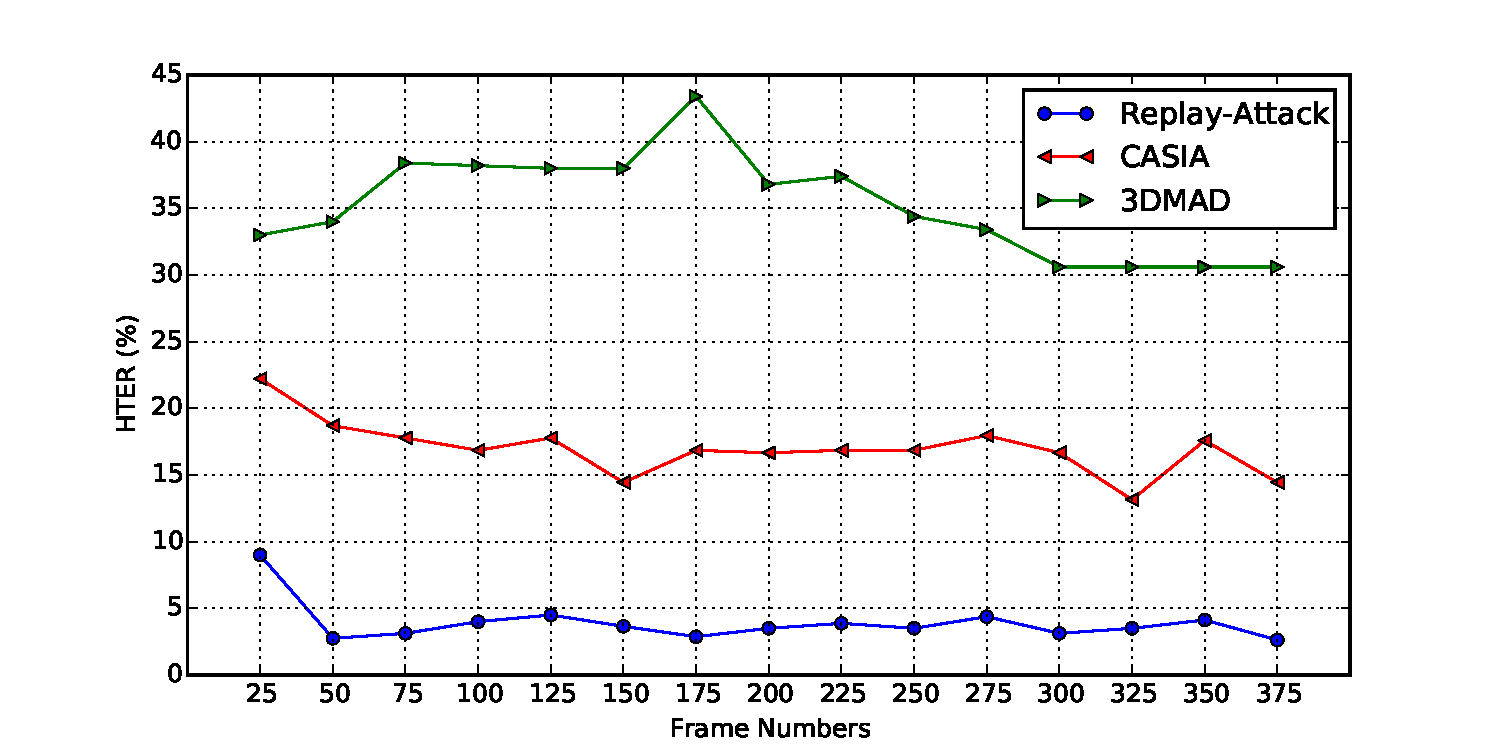
\includegraphics[width=0.45\textwidth]{./figures/n_frames}
\caption{Results in terms of HTER (\%) of the proposed method for different video input length for Replay-Attack, CASIA and 3DMAD datasets.}
\label{fig:n_frames}
\end{figure}

\subsubsection{Cross-Dataset Evaluation}\label{subsec:OtherDatabase}
\minor{In this section, we discuss the performance of the proposed method considering a more difficult scenario (cross-dataset), in which the proposed method is trained with one dataset but it is tested on a different dataset with different acquisition conditions. In this experiment, all datasets used during the training were randomly divided into training and development sets in a proportion of $80\%$ and $20\%$, respectively. The development set is used to estimate the EER threshold that is necessary to calculate the HTER during the test.}

Table~\ref{tab:cross-dataset} shows the results using the cross-dataset protocol. The results indicate that the proposed method presents better generalization when trained with CASIA, with a mean HTER of $40.17\%$. We believe this occurred due to more variability of the type of attacks and video quality in the CASIA dataset, which enriches the training. This dataset contains warped-, cut- and video-based attacks performed with spoofed samples of different quality: low, normal and high quality. Such characteristics enables a better generalization of the method when CASIA is used for training.

{In turn, the best performance when testing the CASIA and 3DMAD datasets was obtained when training with UVAD dataset, another rich dataset for training. Although this dataset contains only video-based spoofing attacks, it has comprises different sensors (for capturing and recapturing the biometric samples) and display devices used during the attempted attacks. We believe that such variability adds different sensor-intrinsic noise levels to the training samples, which contribute to build a more robust classification model.}

{With regard to the more modest generalization presented during the test of the 3DMAD dataset, we believe that it is due to the absence of some artifacts that are commonly found in samples from photo-based and video-based attacks (e.g., blurring, flickering effects) that were not found in the attempted attack video from 3D masks. In addition, spoofing attacks performed with masks are less likely to add temporal disturbances similar to those added when the impostor presents the fake samples, by hand, using a monitor or a photo.}

\minor{Finally, Table~\ref{tab:cross_comparison} shows a comparison among the obtained results reported in the literature. Except for the correlation method, all others present a better performance when they are trained with CASIA. Once again, we believe that our method performs better when training with CASIA because such dataset is more heterogeneous than Replay-Attack. The Correlation~\cite{Anjos:IJCB:2011} and LBP-TOP~\cite{Chingovska:BIOSEG:2012} methods aim to characterize temporal information, similarly to the proposed method, and the results of both methods emphasize the difficulty in characterizing such information completely. In this protocol, besides handling data from different sensors, all methods have to deal with different lighting conditions and background.}

%
%%
%\begin{table}[!htb]
%\scriptsize
%\centering
%%\linethickness{1.5mm}
%\caption{Results in terms of HTER obtained with our method using the cross-dataset Protocol.}
%\label{table:cross}
%\begin{tabular}{lccc}
%\toprule
%\textbf{Datasets} & FAR & FRR & HTER \\
%\toprule
%CASIA  & 11.11 & 83.33 & 47.22 \\
%3DMAD  & 29.41 & 52.94 & 41.18 \\
%UVAD   & 1.34  & {87.17} & {44.26} \\
%\bottomrule
%\end{tabular}
%\end{table}
%
\begin{table*}[!ht]
	\centering
	\footnotesize
	\caption{Results obtained with the cross-dataset protocol and using the overall test sets of each dataset.}
	\label{tab:cross-dataset}	
	\begin{tabular}{cccccc}
		\topline
		\headcol \textbf{Train} & \textbf{Test} & \textbf{FAR (\%)} & \textbf{FRR (\%)} & \textbf{HTER (\%)} & \textbf{Mean HTER (\%)} \\  
		\midline
		%
		& 3DMAD         & 88.00 & 4.00  & 46.00 & \\
		\rowcol 						& Replay-Attack & 32.50 & 36.25 & \textbf{34.38} & \\
		\multirow{-3}{*}{CASIA}         & UVAD          & 38.61 & 41.67 & \textbf{40.14} & \multirow{-3}{*}{ $40.17\%$ } \\
		%
		\hline
		\rowcol									& 3DMAD & 52.00 & 44.00 & 48.00 & \\
		\rowcol									& CASIA & 0.00 & 100.0 & 50.00 & \\
		\rowcol \multirow{-3}{*}{Replay-Attack} & UVAD  & 5.74 & 83.33  & 44.54 & \multirow{-3}{*}{ $47.45\%$ } \\
		%
		\hline
		& 3DMAD         & 84.00 & 4.00  & \textbf{44.00} & \\
		\rowcol							& CASIA         & 13.70 & 63.33 & \textbf{38.52} & \\										
		\multirow{-3}{*}{UVAD}          & Replay-Attack & 79.25 & 6.25 & 42.75  & \multirow{-3}{*}{ $41.76\%$ } \\
		\bottomline 
	\end{tabular} 
\end{table*}
%

%The results show that our method is still not the final word considering a cross-dataset validation (training with one dataset and testing in a different dataset). However, according to other results reported in the literature recently, this behavior is expected, as reported by Pereira et al.~\cite{Pereira:ICB:2013}, whose results in Table~\ref{table:cross_compar} corroborate our findings. We believe that this difficulty of the methods in classifying data from other datasets, not seen during training, is partly because of the different conditions for the acquisition of real samples and recapture of false samples. Therefore, we recommend that either our method is optimized according to the target operational setup or that the method is trained using a good representation of the operational setup of the testing, in other words, the training must comprise examples of situations that could appear during testing. The more complex is the training set the more likely the method will generalize.

%Finally, note that we are not proposing the final word on cross-dataset evaluation. This is a much more challenging problem and here we only touch the tip of the iceberg. Much more work still needs to be done in this direction from all of the research community.
%
%\begin{table}[!htb]
%\scriptsize
%\centering
%%\linethickness{1.5mm}
%\caption{Cross-dataset evaluation comparison of the proposed method with the ones reported in~\cite{Pereira:ICB:2013} for CASIA dataset.}
%\label{table:cross_compar}
%\begin{tabular}{lr}
%\toprule
%\textbf{Datasets} & HTER (\%) \\
%\toprule
%Our method              	 & 47.22   \\
% \hline
%Correlation Motion           & 48.28 \\
%$LBP_{8,1}^{u2}$             & 57.90  \\
%$LBP-TOP_{8,8,8,1,1,1}^{u2}$  & 61.33 \\
%\bottomrule
%\end{tabular}
%\end{table}

%UVAD dataset which contains attempted attacks performed with high quality devices. With this experimental protocol, we obtain an AUC of $94.86\%$ and a HTER of $12.50\%$, considering all attempted attack videos contained on the UVAD dataset. Fig.~\ref{fig:uvad_barplots} shows the results for each sensor acquisition and display devices in the UVAD dataset. The proposed method was capable of capturing noise and artifacts added in the synthetic biometric samples even when the attempted attacks are performed with high quality videos, for different display devices used in the attacks and different biometric sensors. We can conclude that the assumptions made in this work, regarding the perturbations in the frequency components of the signal captured by the acquisition sensor caused by adding noise and artifacts are consistent and generalizable to other attack scenarios.
%%
%\begin{figure*}[!htb]
%\centering
%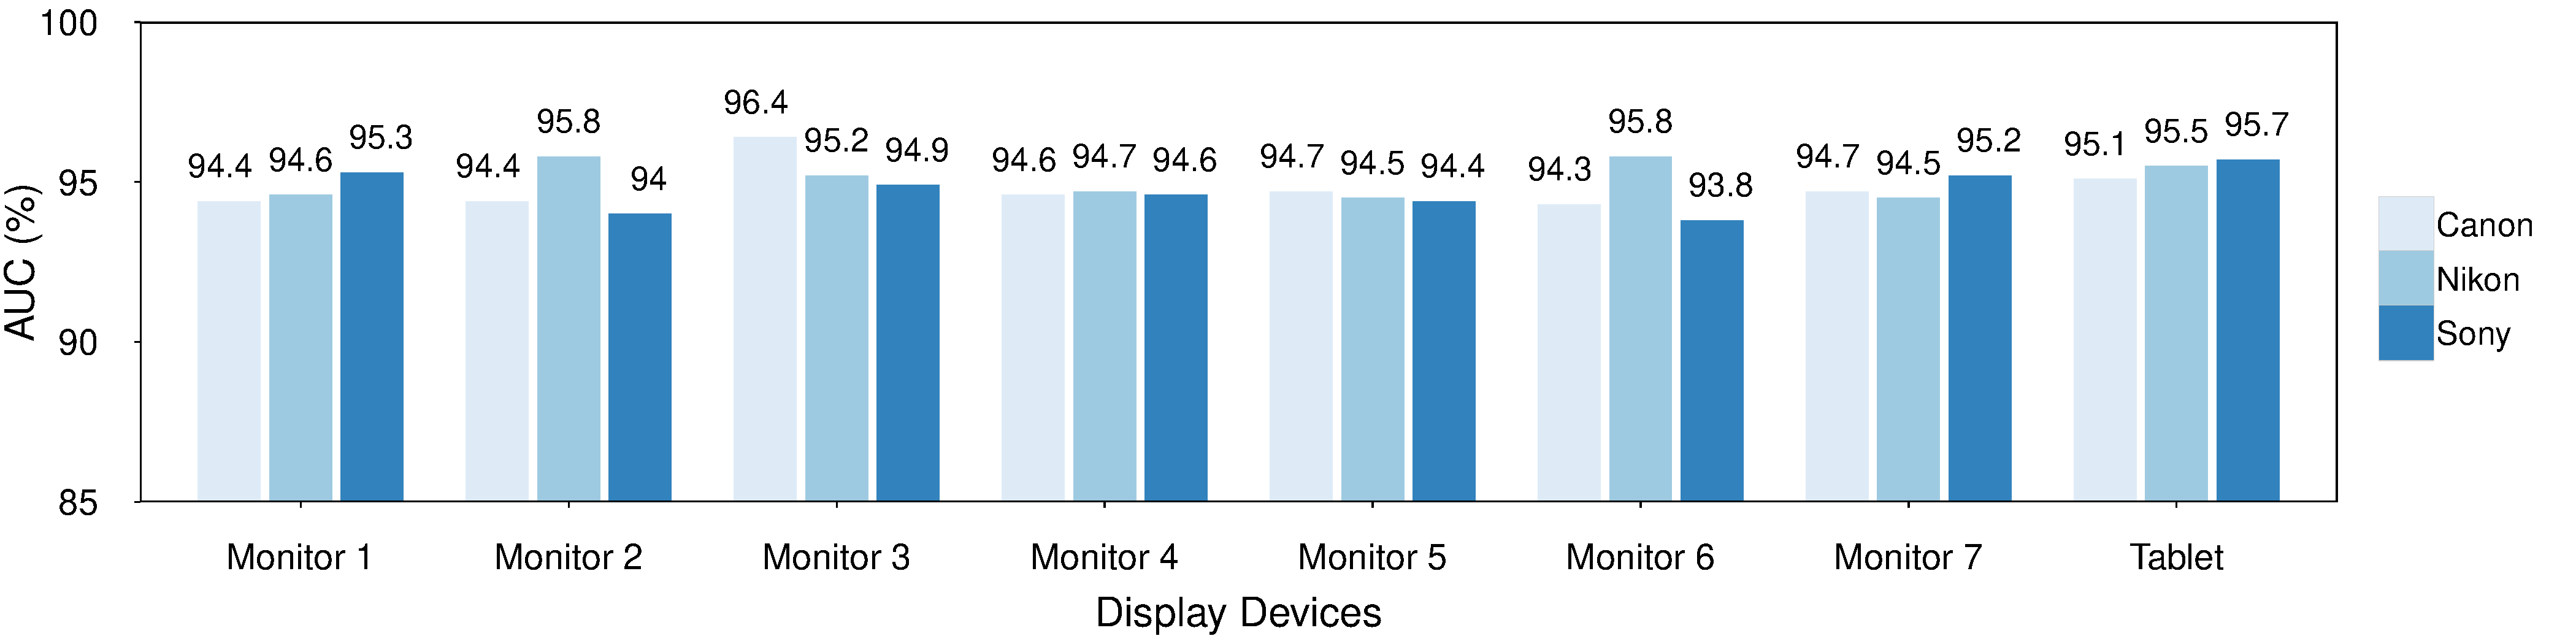
\includegraphics[width=0.99\textwidth]{UVAD_Barplot.pdf}
%\caption{Results (AUC) of the cross-dataset experiment analyzing the different attacks presents on the UVAD dataset. The attacks were performed in three sensor acquisition using eight different display devices.%\newtodo{Remover o fundo cinza.}
%}
%\label{fig:uvad_barplots}
%\end{figure*}

%\newpage
\section{Conclusions and Future Work}
\label{sec:conclusions}

In this work, we investigated two deep representation research approaches for detecting spoofing in different biometric modalities. On one hand, we approached the problem by learning representations directly from the data through architecture optimization with a final decision-making step atop the representations. On the other, we sought to learn filter weights for a given architecture using the well-known back-propagation algorithm. As the two approaches might seem naturally connected, we also examined their interplay when taken together. In addition, we incorporated our experience with architecture optimization as well as with training filter weight for a given architecture into a more interesting and adapted network, \emph{spoofnet}.  

Experiments showed that these approaches achieved outstanding classification results for all problems and modalities outperforming the state-of-the-art results in eight out of nine benchmarks.
Interestingly, the only case for which our approaches did not achieve SOTA results is for the Biosec benchmark. However, in this case, it is possible to achieve a 98.93\% against 100.0\% accuracy of the literature.
These results support our hypothesis that the conception of data-driven systems using deep representations able to extract semantic and vision meaningful features directly from the data is a promising venue. Another indication of this comes from the initial study we did for understanding the type of filters generated by the learning process. Considering the fingerprint case, learning directly from data, it was possible to come up with discriminative filters that explore the blurring artifacts due to recapture. This is particularly interesting as it is in line with previous studies using custom-tailored solutions~\cite{Galbally:TIP:2014}.

It is important to emphasise the interplay between the architecture and filter optimization approaches for the spoofing problem.
It is well-known in the deep learning literature that when thousands of samples are available for learning, the filter learning approach is a promising path. Indeed, we could corroborate this through fingerprint benchmarks that considers a few thousand samples for training. However, it was not the case for faces and two iris benchmarks which suffer from the small sample size problem (SSS) and subject variability hindering the filter learning process. In these cases, the architecture optimization approach was able to learn representative and discriminative features providing comparable spoofing effectiveness to the SOTA results in almost all benchmarks, and specially outperforming them in three out of four SOTA results when the filter learning approach failed. It is worth mentioning that sometimes it is still possible to learn meaningful features from the data even with a small sample size for training. We believe this happens in more well-posed datasets with less variability between training/testing data as it is the case of MobioBIOfake benchmark in which the AO approach achieved 99.38\% just 0.37\% behind the SOTA result. 

As the data tell it all, the decision to which path to follow can also come from the data. Using the evaluation/validation set during training, the researcher/developer can opt for optimizing architectures, learn filters or both. If training time is an issue and a solution must be presented overnight, it might be interesting to consider an already learned network that incorporates some additional knowledge in its design. In this sense, \emph{spoofnet} could be a good choice. In all cases, if the developer can incorporate more training examples, the approaches might benefit from such augmented training data. 

%Although it is more computationally expensive than some existing custom-tailored solutions, our approach is robust to learn representations directly from the data and this is a powerful way of dealing with big data.
%The more data we can collect over time across different modalities, the better and more discriminative will be the representation learning and, consequently, the decision-making process. 
%Moreover, the very fact that the representations are learned directly from the data implies that there is no need for a specialist in each modality or databases for achieving promising results or even outperforming the state-of-the-art methods. 
%If specialist knowledge is available, it can be combined with the proposed solution to provide better-quality training samples and push the solution even further. 

The proposed approaches can also be adapted to other biometric modalities not directly dealt with herein. The most important difference would be in the input type of data since all discussed solutions directly learn their representations from the data.

For the case of iris spoofing detection, here we dealt only with iris spoofing printed attacks and some experimental datasets using cosmetic contact lenses have recently become available allowing researchers to study this specific type of spoofing~\cite{Bowyer:Computer:2014,Yadav:TIFS:2014}. 
For future work, we intend to evaluate such datasets using the proposed approaches here and also consider other biometric modalities such as palm, vein, and gait.

Finally, it is important to take all the results discussed herein with a grain of salt. We are not presenting the final word in spoofing detection. In fact, there are important additional research that could finally take this research another step forward. We envision the application of deep learning representations on top of pre-processed image feature maps (e.g., LBP-like feature maps, acquisition-based maps exploring noise signatures, visual rhythm representations, etc.). With an $n$-layer feature representation, we might be able to explore features otherwise not possible using the raw data. In addition, exploring temporal coherence and fusion would be also important for video-based attacks.

\appendices

\section{Convolutional Network Operations}
\label{sec:convnet_ops}

Our networks use classic convolutional operations that can be viewed as linear and non-linear image processing operations. When stacked, these operations essentially extract higher level representations, named \emph{multiband images}, whose pixel attributes are concatenated into high-dimensional feature vectors for later pattern recognition.\footnote{This appendix describes convolutional networks from an image processing perspective, therefore the use of terms like image \emph{domain}, image \emph{band}, \emph{etc.}}

Assuming $\hat{I}=(D_I,\vec{I})$ as a multiband image, where $D_I \subset Z^2$ is the image domain and $\vec{I}(p)=\{I_1(p),I_2(p),\ldots, I_m(p)\}$ is the attribute vector of a $m$-band pixel $p=(x_p,y_p)\in D_I$, the aforementioned operations can be described as follows.

\subsubsection{Filter Bank Convolution}

Let ${\cal A}(p)$ be a squared region centered at $p$ of size $L_{\cal A} \times L_{\cal A}$, such that ${\cal A} \subset D_I$ and $q\in {\cal A}(p)$ iff $\max(|x_q-x_p|,|y_q-y_p|)\leq (L_{\cal A}-1)/2$.
Additionally, let $\Phi=({\cal A},W)$ be a filter with weights $W(q)$ associated with pixels $q\in {\cal A}(p)$.
In the case of multiband filters, filter weights can be represented as vectors $\vec{W}_i(q)=\{w_{i,1}(q),w_{i,2}(q),\ldots,w_{i,m}(q)\}$ for each filter $i$ of the bank, and a multiband filter bank $\Phi = \{\Phi_1, \Phi_2, \ldots, \Phi_n\}$ is a set of filters $\Phi_i=({\cal A},\vec{W}_i)$, $i=\{1,2,\ldots,n\}$.

The convolution between an input image $\hat{I}$ and a filter $\Phi_i$ produces a band $i$ of the filtered image $\hat{J}=(D_J,\vec{J})$, where $D_J \subset D_I$ and $\vec{J}=(J_1,J_2,\ldots,J_n)$, such that for each $p\in D_J$,
\begin{equation}
J_i(p) = \sum_{\forall q\in {\cal A}(p)} \vec{I}(q)\cdot \vec{W}_i(q).
\end{equation}

\subsubsection{Rectified Linear Activation}

Filter activation in this work is performed by rectified linear units (RELUs) of the type present in many state-of-the-art convolutional architectures~\cite{Krizhevsky:2012,Pinto:2011b} and is defined as
\begin{equation}
J_i(p) = \max(J_i(p),0).
\end{equation}

\subsubsection{Spatial Pooling}

Spatial pooling is an operation of paramount importance in the literature of convolutional networks~\cite{LeCun:1998} that aims at bringing translational invariance to the features by aggregating activations from the same filter in a given region. 

Let ${\cal B}(p)$ be a pooling region of size $L_{\cal B} \times L_{\cal B}$ centered at pixel $p$ and $D_K = D_J/s$ be a regular subsampling of every $s$ pixels $p \in D_J$. We call $s$ the \emph{stride} of the pooling operation. Given that $D_J \subset Z^2$, if $s=2$, $|D_K| = |D_J|/4$, for example.
The pooling operation resulting in the image $\hat{K}=(D_K,\vec{K})$  is defined as 
\begin{equation}
K_i(p) = \sqrt[\alpha]{\sum_{\forall q\in {\cal B}(p)} J_i(q)^{\alpha}}, 
\end{equation}
where $p\in D_K$ are pixels in the new image, $i=\{1,2,\ldots,n\}$ are the image bands, and $\alpha$ is a hyperparameter that controls the sensitivity of the operation. In other words, our pooling operation is the $L_{\alpha}$-norm of values in ${\cal B}(p)$. 
The stride $s$ and the size of the pooling neighborhood defined by $L_{\cal B}$ are other hyperparameters of the operation.

\subsubsection{Divisive Normalization}

The last operation considered in this work is divisive normalization, a mechanism widely used in top-performing convolutional networks~\cite{Krizhevsky:2012,Pinto:2011b} that is based on gain control mechanisms found in cortical neurons~\cite{Geisler:1992}.

This operation is also defined within a squared region ${\cal C}(p)$ of size $L_{\cal C} \times L_{\cal C}$ centered at pixel $p$ such that 
\begin{equation}
O_i(p) = \frac{K_i(p)}{\sqrt{\sum_{j=1}^{n}\sum_{\forall q\in {\cal C}(p)} K_j(q)^2}}
\end{equation}
for each pixel $p\in D_O \subset D_K$ of the resulting image $\hat{O}=(D_O,\vec{O})$. Divisive normalization promotes competition among pooled filter bands such that high responses will prevail even more over low ones, further strengthening the robustness of the output representation $\vec{O}$.


\section*{Acknowledgment}

We thank UFOP, Brazilian National Research Counsil -- CNPq (Grants \#303673/2010-9,  \#304352/2012-8, \#307113/2012-4, \#477662/2013-7, \#487529/2013-8, \#479070/2013-0, and \#477457/2013-4), the CAPES DeepEyes project, S\~ao Paulo Research Foundation -- FAPESP, (Grants \#2010/05647-4, \#2011/22749-8, \#2013/04172-0, and \#2013/11359-0), and Minas Gerais Research Foundation -- FAPEMIG (Grant APQ-01806-13). 
D. Menotti thanks FAPESP for a grant to acquiring two NVIDIA GeForce GTX Titan Black with 6GB each.
We also thank NVIDIA for donating five GPUs used in the experiments, a Tesla K40 with 12GB to A. X. Falc{\~a}o, two GeForce GTX 680 with 2GB each to G. Chiachia, and two GeForce GTX Titan Black with 6GB each to D. Menotti.

\ifCLASSOPTIONcaptionsoff
  \newpage
\fi

%\IEEEtriggeratref{8}
%\IEEEtriggercmd{\enlargethispage{-5in}}

%\balance
\bibliographystyle{IEEEtran}
\bibliography{spoofing,iris,faces,fingerprint}
%IEEEabrv,


\begin{IEEEbiography}[{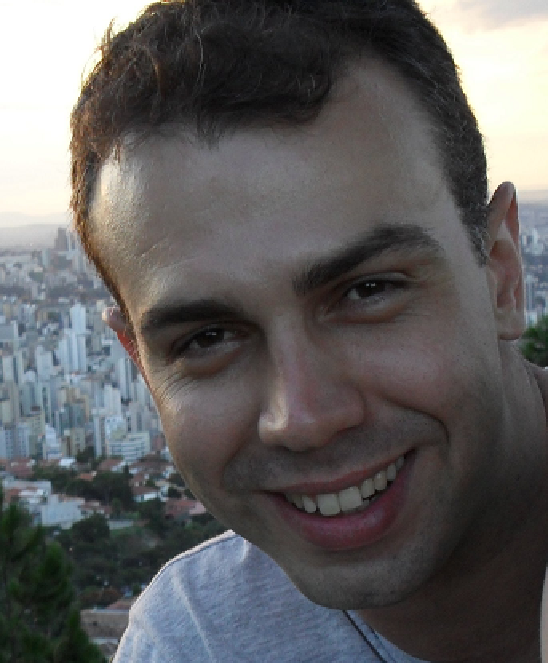
\includegraphics[width=1in,height=1.25in,clip,keepaspectratio]{photo-menotti}}]{David Menotti} received his Computer Engineering and Informatics Applied Master degrees from the Pontif\'icia Universidade Cat\'olica do Paran\'a (PUCPR), Curitiba, Brazil, in 2001 and 2003, respectively.
In 2008, he received his co-tutelage PhD degree in Computer Science from the Federal University of Minas Gerais (UFMG), Belo Horizonte, Brazil and the Universit\'e Paris-Est/Groupe ESIEE, Paris, France.
He is an associate professor at the Computing Department (DECOM), Universidade Federal de Ouro Preto (UFOP), Ouro Preto, Brazil, since August 2008. 
From June 2013 to May 2014 he has been on his sabbatical year at Institute of Computing, University of Campinas (UNICAMP), Campinas, Brazil, as a post-doc / collaborator researcher supported by FAPESP (grant 2013/4172-0).
Currently, he is working as a permanent and collaborator professor at the Post-Graduate Program in Computer Science DECOM-UFOP and DCC-UFMG, respectively.

His research interests include image processing, pattern recognition, computer vision, and information retrieval.
\end{IEEEbiography}

%\vspace{-18pt}
\begin{IEEEbiography}[{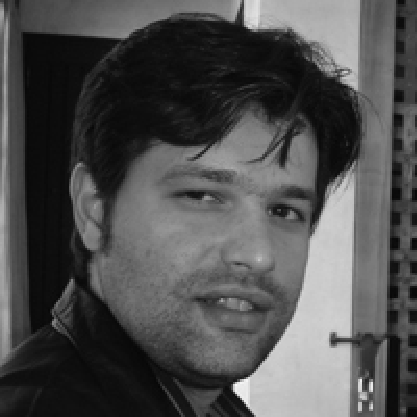
\includegraphics[width=1in,height=1.25in,clip,keepaspectratio]{photo-chiachia}}]{Giovani Chiachia}  
Giovani Chiachia is a post-doctorate researcher at University of Campinas, Brazil.
His main research interest is to approach computer vision and other artificial intelligence tasks with brain-inspired machine learning techniques. 
He received his B.Sc. (2005) and his M.S. (2009) degrees from São Paulo State University and his Ph.D. in Computer Science from the University of Campinas (2013).
He held research scholar positions at the Fraunhofer Institute IIS and at Harvard University as part of his graduate work, and was awarded first place for the performance of his face recognition system in the IEEE Intl. Conf. on Biometrics (2013). 
Beyond his research experience, Dr. Chiachia has a large experience in the IT industry, managing and being part of teams working on projects from a wide range of complexities and scales.
\end{IEEEbiography}

%\vspace{-18pt}
\begin{IEEEbiography}[{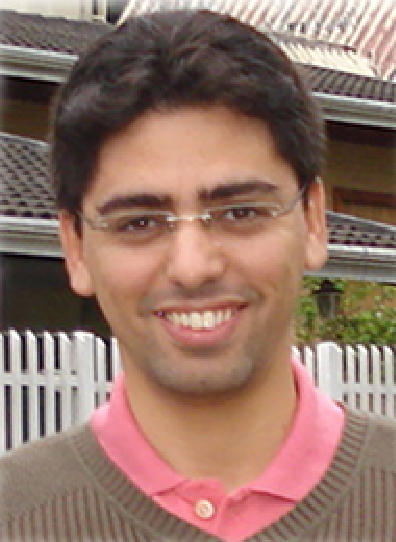
\includegraphics[width=1in,height=1.25in,clip,keepaspectratio]{photo-pinto}}]{Allan da Silva Pinto} 
Allan Pinto received the B.Sc. degree in Computer Science from University of São Paulo (USP), Brazil, in 2011, and the M.Sc. degree in Computer Science from University of Campinas (Unicamp), Brazil, in 2013. Currently, he is a Ph.D. Student, also in Computer Science, at Institute of Computing, Unicamp, Brazil. 

His research focuses on the areas of image and video analysis, computer forensics, pattern recognition, and computer vision in general, with a particular interest in spoofing detection in biometric systems.
\end{IEEEbiography}

%\vspace{-18pt}
\begin{IEEEbiography}[{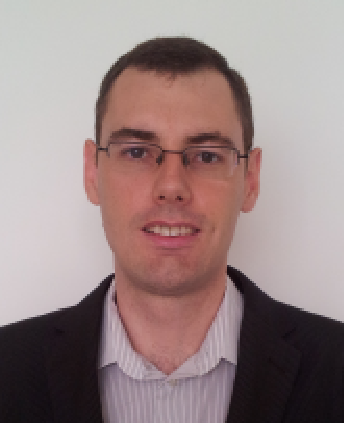
\includegraphics[width=1in,height=1.25in,clip,keepaspectratio]{photo-schwartz}}]{William Robson Schwartz} 
William Robson Schwartz received his Ph.D. degree in Computer Science from University of Maryland, College Park, USA. He received his B.Sc. and M.Sc. degrees in Computer Science from the Federal University of Parana, Curitiba, Brazil.
He is currently a professor in the Department of Computer Science at the Federal University of Minas Gerais, Brazil.

His research interests include computer vision, computer forensics, biometrics and image processing.
\end{IEEEbiography}

%\vspace{-18pt}
\begin{IEEEbiography}[{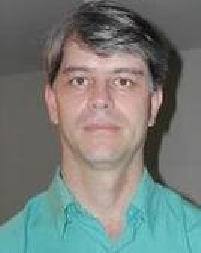
\includegraphics[width=1in,height=1.25in,clip,keepaspectratio]{photo-pedrini}}]{Helio Pedrini} 
Helio Pedrini received his Ph.D. degree in Electrical and Computer Engineering from Rensselaer Polytechnic Institute, Troy, NY, USA. 
He received his M.Sc. degree in Electrical Engineering and his B.Sc. in Computer Science, both from the University of Campinas, Brazil. 
He is currently a professor in the Institute of Computing at the University of Campinas, Brazil. 

His research interests include image processing, computer vision, pattern recognition, machine learning, computer graphics, computational geometry.
\end{IEEEbiography}

%\vspace{-18pt}
\begin{IEEEbiography}[{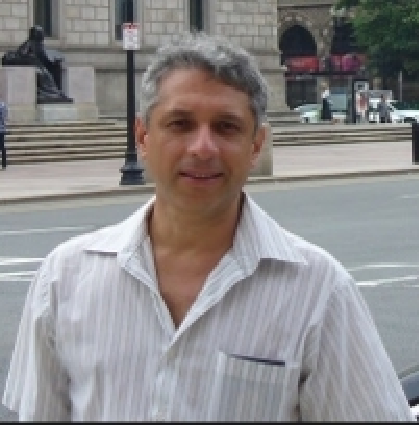
\includegraphics[width=1in,height=1.25in,clip,keepaspectratio]{photo-falcao}}]{Alexandre Xavier Falcão} 
Alexandre Xavier Falcao is full professor at the Institute of Computing, University of Campinas, Campinas, SP, Brazil. 
He received a B.Sc. in Electrical Engineering from the Federal University of Pernambuco, Recife, PE, Brazil, in 1988. He has worked in biomedical image processing, visualization and analysis since 1991. 
In 1993, he received a M.Sc. in Electrical Engineering from the University of Campinas, Campinas, SP, Brazil. 
During 1994-1996, he worked with the Medical Image Processing Group at the Department of Radiology, University of Pennsylvania, PA, USA, on interactive image segmentation for his doctorate. 
He got his doctorate in Electrical Engineering from the University of Campinas in 1996. 
In 1997, he worked in a project for Globo TV at a research center, CPqD-TELEBRAS in Campinas, developing methods for video quality assessment. 
His experience as professor of Computer Science and Engineering started in 1998 at the University of Campinas. 

His main research interests include image/video processing, visualization, and analysis; graph algorithms and dynamic programming; image annotation, organization, and retrieval; machine learning and pattern recognition; and image analysis applications in Biology, Medicine, Biometrics, Geology, and Agriculture.
\end{IEEEbiography}

%\vspace{-18pt}
\begin{IEEEbiography}[{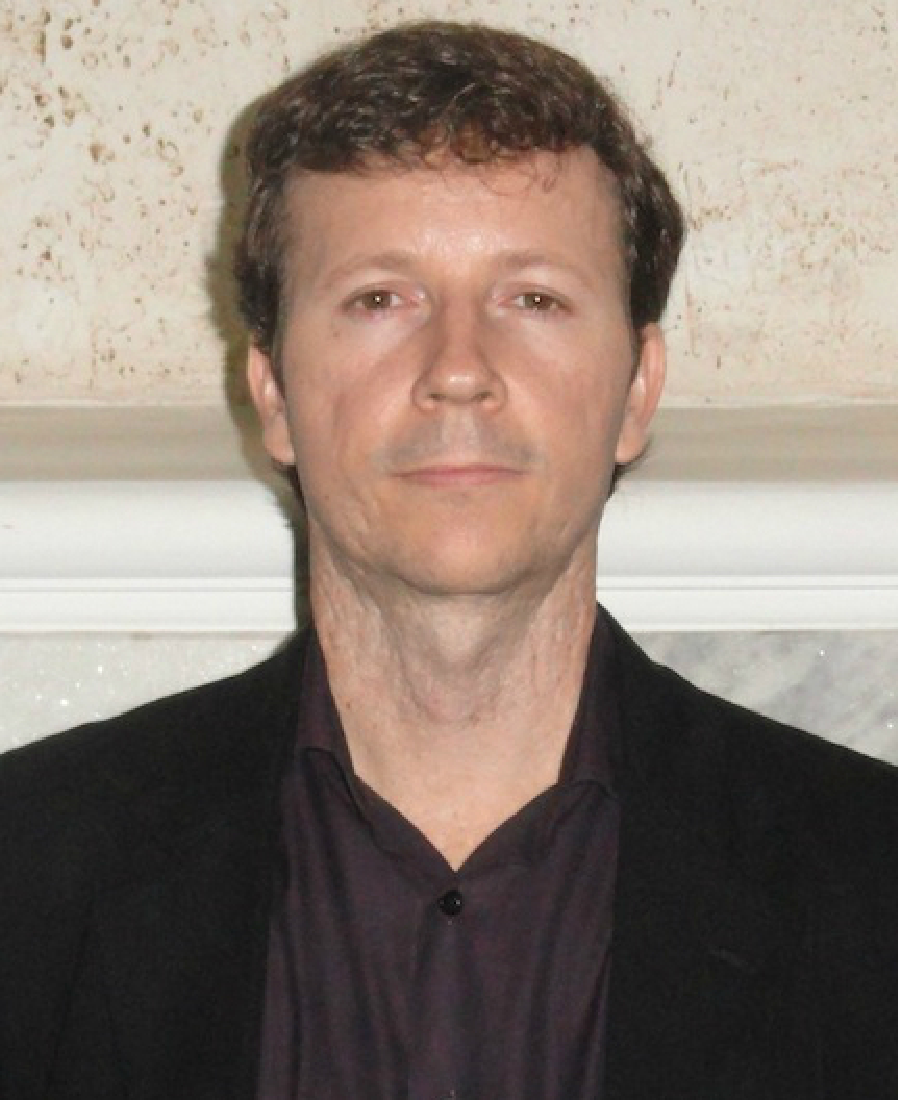
\includegraphics[width=1in,height=1.25in,clip,keepaspectratio]{photo-rocha}}]{Alexandre de Rezende Rocha}
Anderson de Rezende Rocha received his B.Sc (Computer Science) degree from Federal University of Lavras (UFLA), Brazil in 2003. He received his M.S. and Ph.D. (Computer Science) from University of Campinas (Unicamp), Brazil, in 2006 and 2009, respectively. 
Currently, he is an assistant professor in the Institute of Computing, Unicamp, Brazil. 

His main interests include digital forensics, reasoning for complex data, and machine  intelligence. 
He has actively worked as a program committee member in several important Computer Vision, Pattern Recognition, and Digital Forensics events. 
He is an associate editor of the Elsevier Journal of Visual Communication and Image Representation (JVCI) and a Leading Guest Editor for EURASIP/Springer Journal on Image and Video Processing 
(JIVP) and IEEE Transactions on Information Forensics and Security (T.IFS). 
He is an affiliate member of the Brazilian Academy of Sciences (ABC) and the Brazilian Academy of Forensics Sciences (ABCF). 
He is also a Microsoft Research Faculty Fellow and a former member of the IEEE Information Forensics and Security Technical Committee (IFS-TC).
\end{IEEEbiography}
%\balance

\end{document}
